%%% Laboratory	 Notes
%%% Template by Mikhail Klassen, April 2013
%%% Contributions from Sarah Mount, May 2014
%%% Contributions from Muhammad Davi, September 2022
\documentclass[a4paper]{tufte-handout}
\usepackage{lab_notes}

\title{Practice Big Data}
\date{2022}

\begin{document}
\maketitle
\justifying

%%%%%%%%%%%%%%%%%%%%%%%%%%%%%%%%%%%%%%%%%%%%%%%%%%%%%%%%

\begin{projects}
	\begin{description}
		\item [Muhammad Davi, S.Kom., M.Cs.] adalah sebagai dosen pengampu matakuliah practice big data\footnote{Dosen Prodi Teknologi Rekayasa Komputer Jaringan, Jurusan Teknologi Informasi dan Komputer, Politeknik Negeri Lhokseumawe}.
		\item [Peserta dan Kelompok] matakuliah practice big data adalah sebegai berikut:

\begin{table}[!ht]
\caption{Peserta dan Kelompok Matakuliah Practice Big Bata}
\label{tab:peserta}
\centering
\begin{tabular}{ll} 
\toprule
Nama &	Akun Github\\
\midrule
Kelompok 1\\
\midrule
Adinda Awaliah			& \url{https://github.com/AdindaAwaliah} \\
Adjie Yusmunandar		& \url{https://github.com/AdjieYusmunandar} \\
Arya Saputra			& \url{https://github.com/AryaSpt} \\
Jihan Dwi Sarah			& \url{https://github.com/jhndsrh} \\
\midrule
Kelompok 2\\
\midrule
Muhammad Munawir		& \url{https://github.com/Munawir027} \\
Muhammad Ikrammullah	& \url{https://github.com/Ikram160302} \\
M. Ikhsan				& \url{https://github.com/Muhammadikhsandev} \\
Zulfahmi				& \url{https://github.com/zulfahmidev} \\
\midrule
Kelompok 3\\
\midrule
Nadzura Kumaira			& \url{https://github.com/NadzuraKumaira} \\
Nurani Harum Fardaniah	& \url{https://github.com/fardaniahnh} \\
Nuraula Tafiza			& \url{https://github.com/olala17} \\
Nurul Aflah				& \url{https://github.com/Nurulaflahhh} \\
Faiza Yuwafiqi			& \url{https://github.com/faizayuwafiqi} \\
\midrule
Kelompok 4\\
\midrule
Rauzatinur Syah			& \url{https://github.com/rauzatinursyah} \\
Resha Russita			& \url{https://github.com/resharussita} \\
Rizki Ilhami			& \url{https://github.com/RIZKIINC} \\
Taravia Fauzah			& \url{https://github.com/traviafzah} \\
\midrule
Kelompok 5\\
\midrule
Salsabila Irmanda		& \url{https://github.com/salsabilairmanda17} \\
\textcolor{red}{Siti Hajar Al Zahra	}	& - \\
Syarfani Akbar			& \url{https://github.com/SyarfaniAkbar} \\
Cut Opy Mandalisa		& \url{https://github.com/cutopymdl} \\
\midrule
\end{tabular}
\end{table}
	\end{description}
\end{projects}

%%%%%%%%%%%%%%%%%%%%%%%%%%%%%%%%%%%%%%%%%%%%%%%%%%%%%%%%

\begin{maybe}
\begin{itemize}
\item Waktu, Tempat dan Penilaian


\begin{itemize}
\item Waktu: 13.30 - 16.00, 16.20 - 18.00\footnote{Istirahat dan Sholat Ashar 20 Menit}
\item Tempat: Ruang Lab 3\footnote{Lab Jaringan dan Multimedia di Lantai Dasar Gedung Utama}
\item Penilaian\footnote{Sesuai ketentuan dari Kepala Lab}

\begin{multicols}{2}
\begin{itemize}
\item Responsi Kompetensi
\item Sikap
\item Laporan
\item Seminar
\item UAS
\item Hasil/Benda kerja
\end{itemize}
\end{multicols}
\end{itemize}

\item Sebelum masuk lab wajib berbaris dan berdo'a terlebih dahulu di depan lab.
\item Sebelum perkuliahan dimulai, mahasiswa atau yang mewakili memberi laporan.
\item Setiap keluar lab meminta izin kepada dosen pengampu.
\item Mengikuti Tata Tertib yang berlaku.
\item Referensi

\begin{itemize}
\item Buku Ajar Big Data \citep{Mursyidah2020}.
\end{itemize}

\item Tata Cara Presensi selama Perkuliahan Online

\begin{itemize}
\item Buka repository laporan-practice-big-data melalui akun GitHub masing-masing
\item Lakukan sinkro fork (Sync fork)
\item Buka file {\tt lab\_notes.tex} menggunakan texmaker dan buka file laporan masing-masing
\item Tambahkan kode berikut dan sesuaikan tanggalnya. \\
\textbf{\textcolor{red}{Pastikan kode sudah benar!}}
\begin{lstlisting}
\newday{\textbf{1 Desember 2022}}
\begin{enumerate}
	\item Kendala dan Solusi
	\item Kesimpulan
\end{enumerate}
\end{lstlisting}
\item Lakukan {\tt git add, git commit dan git push}. \\ 
Format \textit{message} saat {\tt git commit} \textit{"Presensi dd-mm-yyyy a.n. Nama"}. Contoh: "Presensi 01-12-2022 a.n. Davi"
\item Buat {\tt pull requests} melalui menu \textbf{Contribute}.
\end{itemize}
\end{itemize}
\end{maybe}

%%%%%%%%%%%%%%%%%%%%%%%%%%%%%%%%%%%%%%%%%%%%%%%%%%%%%%%%
\clearpage
\newday{\#1 - 8 September 2022}

\newthought{Introduction \& Preparation}

Pada pertemuan pertama, kegiatan lab adalah perkenalan dan persiapan kebutuhan untuk praktik big data. Setelah dosen pengampu memperkenalkan diri dan matakuliah yang diajarkan, dilanjutkan perkenalan dari setiap mahasiswa dah hasilnya dapat dilihat pada Tabel \ref{tab:perkenalan}.

\begin{table}[!ht]
\vspace*{.5cm}
\caption{Data Mahasiswa}
\label{tab:perkenalan}
\centering
\begin{tabular}{cllr} 
\toprule
No & Nama 				& Asal Sekolah 				& Alamat\\
\midrule
1 	& Adinda Awaliah	& SMA N 1 Lhokseumawe 		& Cunda \\
2 	& Adjie Yusmunandar	& SMK N 1 Lhokseumawe 		& Paloh Lada \\
3 	& Arya Saputra		& & \\
4 	& Cut Opy Mandalisa	& SMA N 1 Syamtalira Bayu	& Bayu \\
5 	& Faiza Yuwafiqi	& & \\
6 	& Jihan Dwi Sarah	& SMA N 1 Lhokseumawe 		& Panggoi \\
7 	& M. Ikhsan			& SMK N 1 Simpang Kiri 		& Subulussalam \\
\midrule
8 	& Muhammad Ikrammullah		& SMK N 1 Lhokseumawe 	& Banda Sakti \\
9 	& Muhammad Munawir			& SMK N 1 Lhoksukon		& Karing Meurah Mulia \\
10 	& Nadzura Kumaira			& SMK N 2 Lhokseumawe 	& Keude Aceh \\
11 	& Nurani Harum Fardaniah	& SMK N 1 Lhoksukon 	& Buket Hagu \\
12 	& Nuraula Tafiza			& SMK N 1 Lhoksukon 	& Alue Buket \\
13 	& Nurul Aflah				& & \\
14 	& Rauzatinur Syah			& MAS Misbahul Ulum 	& Geudong \\
\midrule
15 	& Resha Russita			& SMA N 1 Lhokseumawe 	& Alue Awe \\
16 	& Rizki Ilhami			& SMK N 1 Lhoksukon 	& Lapang \\
17 	& Salsabila Irmanda		& MAS Misbahul Ulum 	& Alue Awe \\
18 	& Siti Hajar Al Zahra	& & \\
19 	& Syarfani Akbar		& & \\
20 	& Taravia Fauzah		& SMA N 1 Dewantara 	& Blang Naleung Mameh \\
21 	& Zulfahmi				& SMK N 1 Lhokseumawe	& Kuta Makmur \\
\bottomrule
\end{tabular}
\end{table}

\vspace*{.5cm}
Setelah perkenalan, setiap mahasiswa membuat akun github dan akun discord sebagai media komunikasi dan tempat bekerja secara berkelompok. Hasil dari kegiatan tersebut dapat dilihat pada Tabel \ref{tab:peserta} dan Link Server Discord, yaitu \url{https://discord.gg/bJCNpaxv62}.

Tugas di pertemuan pertama adalah menyiapkan \textit{environment} untuk tempat kerja minimal sebagai berikut:
\begin{multicols}{2}
\begin{itemize}
\setlength\itemsep{0em}
\item Processor 2 GHz dual-core
\item RAM sebesar 4 GB
\item Harddisk kosong 25 GB
\item Resolusi layar 1024 x 768
\item \textit{Operating System}: Ubuntu 22.04 LTS
\end{itemize}
\end{multicols}
\hrulefill

%%%%%%%%%%%%%%%%%%%%%%%%%%%%%%%%%%%%%%%%%%%%%%%%%%%%%%%%
\clearpage
\newday{\#2 - 15 September 2022}

\newthought{Instalasi dan Konfigurasi GIT dengan GitHub}

Pada pertemuan kali ini kita belajar install GIT dan konfigurasi GIT dengan GitHub agar dapat menjalankan perintah-perintah GIT melalui lokal dan menyimpan hasil kerjaan kita ke GitHub. Karena pada pertemuan pertama telah membuat akun GitHub, maka pada pertemuan kali ini asumsinya semua sudah memiliki akun GitHub. Setelah itu ikuti beberapa langkah berikut untuk praktikum kali ini.

\begin{enumerate}
\item Install Git \\
Pertema download program Git melalui link ini (\url{https://git-scm.com/download}) sesuai dengan sistem operasi yang digunakan. Bagi pengguna Windows jika proses download sudah selesai, lanjut proses instalasi seperti program windows pada umumnya (Next, Next, Next, sampai selesai).

\item \textit{Generate} SSH-Key \\
Jika instalasi sudah selesai, coba buka Git Bash, maka akan muncul program baru yang mirip dengan Terminal atau Command Prompt (CMD) kita sebut Git Bash. Kemudian jalankan perintah berikut untuk \textit{generate ssh-key}.

{\tt ssh-keygen -t ed25519 -C "email@akun.github"} \\

Ganti {\tt email@akun.github} dengan email yang terdaftar pada akun GitHub. Selanjutnya jika muncul beberapa pertanyaan seperti berikut ini tekan [enter].

{\tt > Enter a file in which to save the key (/Users/YOU/.ssh/id\_ed25519:} \\
{\tt > Enter passphrase (empty for no passphrase):} \\
{\tt > Enter same passphrase again:}

Jika proses diatas berhasil maka terbentuk folder baru dengan nama {\tt .ssh}. Didalam folder tersebut terdapat \textit{private key} dan \textit{public key}. Bukan file \textit{public key} (id\_ed25519.pub) dan \textit{copy} isi dari file tersebut.

\item Menambahkan SSH-Key ke Akun GitHub \\
Untuk menambahkan SSH-Key ke akun GitHub pertama login terlebih dahulu. Setelah berhasil login klik pada gambar profil sehingga tampil menu dropdown seperti pada Gambar \ref{gam:langkah-ssh} nomor 1. Selanjutnya pilih menu \textbf{Setting} sepertin yang ditunukan pada nomor 2. Setelah memilih menu \textbf{Setting} maka muncul halaman setting dengan menu di sidebar sebelah kiri. Pada menu sebelah kiri pilih menu \textbf{SSH and GPG keys} seperti pada nomor 3. Kemudian klik tombol \textbf{New SSH key} maka akan muncul form menambahkan SSH seperti yang diperlihatkan pada Gambar \ref{gam:form-ssh}.

\begin{figure}[!ht]
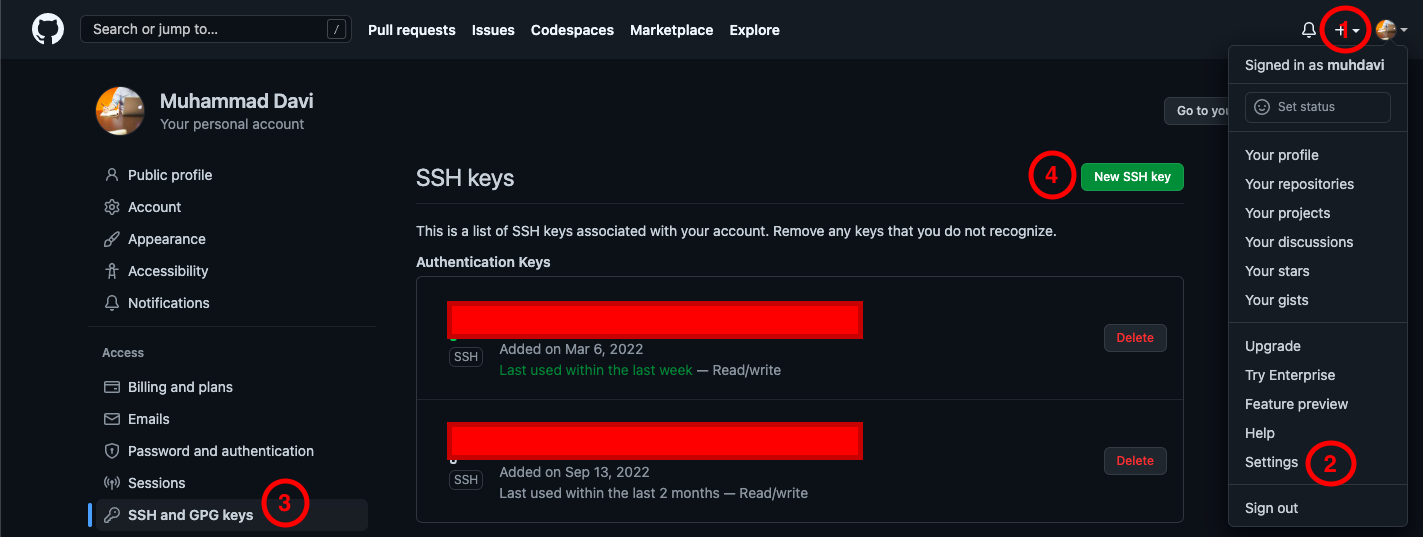
\includegraphics[width=\textwidth]{gtihub-1}
\caption{Lankah-langkah Menambah SSH-Key di GitHub}
\label{gam:langkah-ssh}
\end{figure}

Kode SSH-Key yang telah di-\textit{copy} pada langkah sebelumnya \textit{paste}-kan kode tersebut pada isian \textbf{Key} dan beri judul SSH-Key pada isian \textbf{Title}. Setelah semua diisi klik tombol \textbf{Add SSH key} untuk menyimpan SSH-Key baru tersebut.

\begin{figure}[!ht]
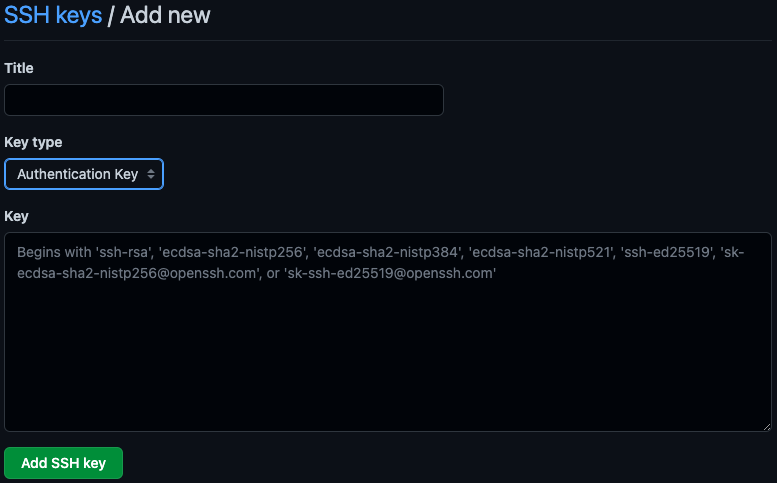
\includegraphics[width=\textwidth]{github-2}
\caption{Form Penambahan SSH-Key di GitHub}
\label{gam:tambah-ssh}
\end{figure}

Untuk menguji bahwa penambahan SSH-Key telah berhasil coba lakukan {\tt git push} untuk repositori laporan practice big data dari akun masing-masing. Untuk lebih jelasnya tentang GIT dapat membaca catatan pada link berikut \url{https://muhdavi.github.io/learn-git/}.
\end{enumerate}

\begin{figure}[!ht]
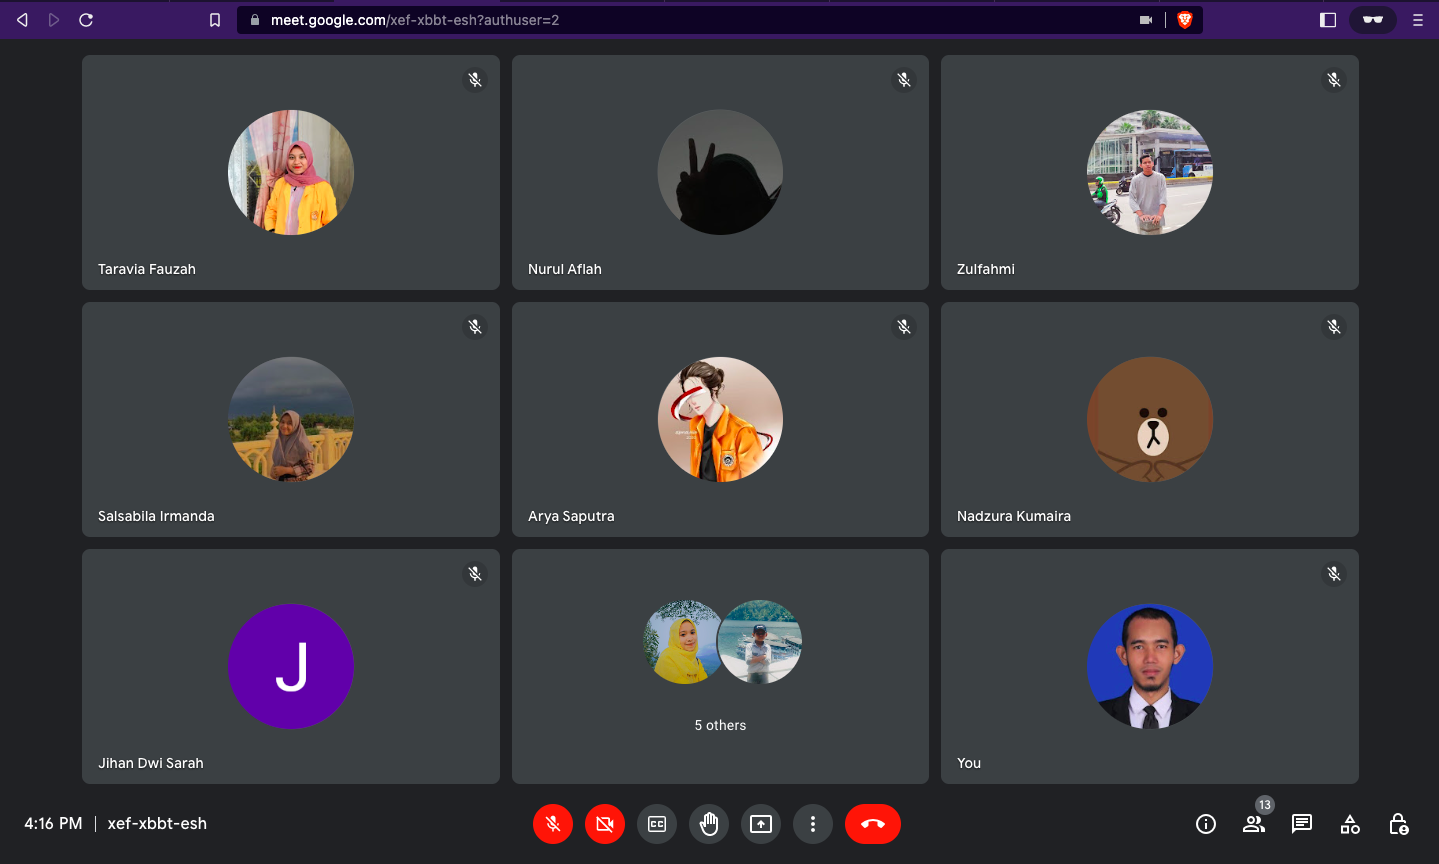
\includegraphics[width=.95\textwidth]{24-11-2022}
\caption{Perkuliahan Daring via Google Meet}
\label{gam:perkuliahan-24-11}
\end{figure}

\vspace*{-.5cm}
\hrulefill

%%%%%%%%%%%%%%%%%%%%%%%%%%%%%%%%%%%%%%%%%%%%%%%%%%%%%%%%
\clearpage
\newday{\#3 - 22 September 2022}
\newday{\#4 - 24 November 2022 menggantikan 29 September 2022}
\newday{\#5 - 25 November 2022 menggantikan 6 Oktober 2022}

\newthought{Instalasi dan Konfigurasi GIT dengan GitHub - Lanjutan}

Mahasiswa yang sudah berhasil konfigurasi Git dengan GitHub dan melakukan {\tt Pull Request}:
\begin{multicols}{2}
\begin{enumerate}
\item Rizki Ilhami
\item Rauzatinur Syah $\star$
\item Taravia Fauzah
\item Resha Russita $\star$
\item Nurani Harum Fardaniah $\star$
\item Adinda Awaliah $\star$
\item Salsabila Irmanda $\star$
\item M. Ikhsan
\item Jihan Dwi Sarah $\star$
\item Cut Opy Mandalisa $\star$
\item Zulfahmi
\item Muhammad Munawir
\item Nuraula Tafiza
\item Muhammad Ikrammullah
\item Nadzura Kumaira
\item Adjie Yusmunandar
\end{enumerate}
\end{multicols}

\noindent
Berikut beberapa mahasiswa yang belum melakukan {\tt Pull Request}:
\begin{multicols}{2}
\begin{enumerate}
\item Arya Saputra
\item Faiza Yuwafiqi
\item Nurul Aflah
\item \textcolor{red}{Siti Hajar Al Zahra}
\item Syarfani Akbar
\end{enumerate}
\end{multicols}

\begin{figure}[!ht]
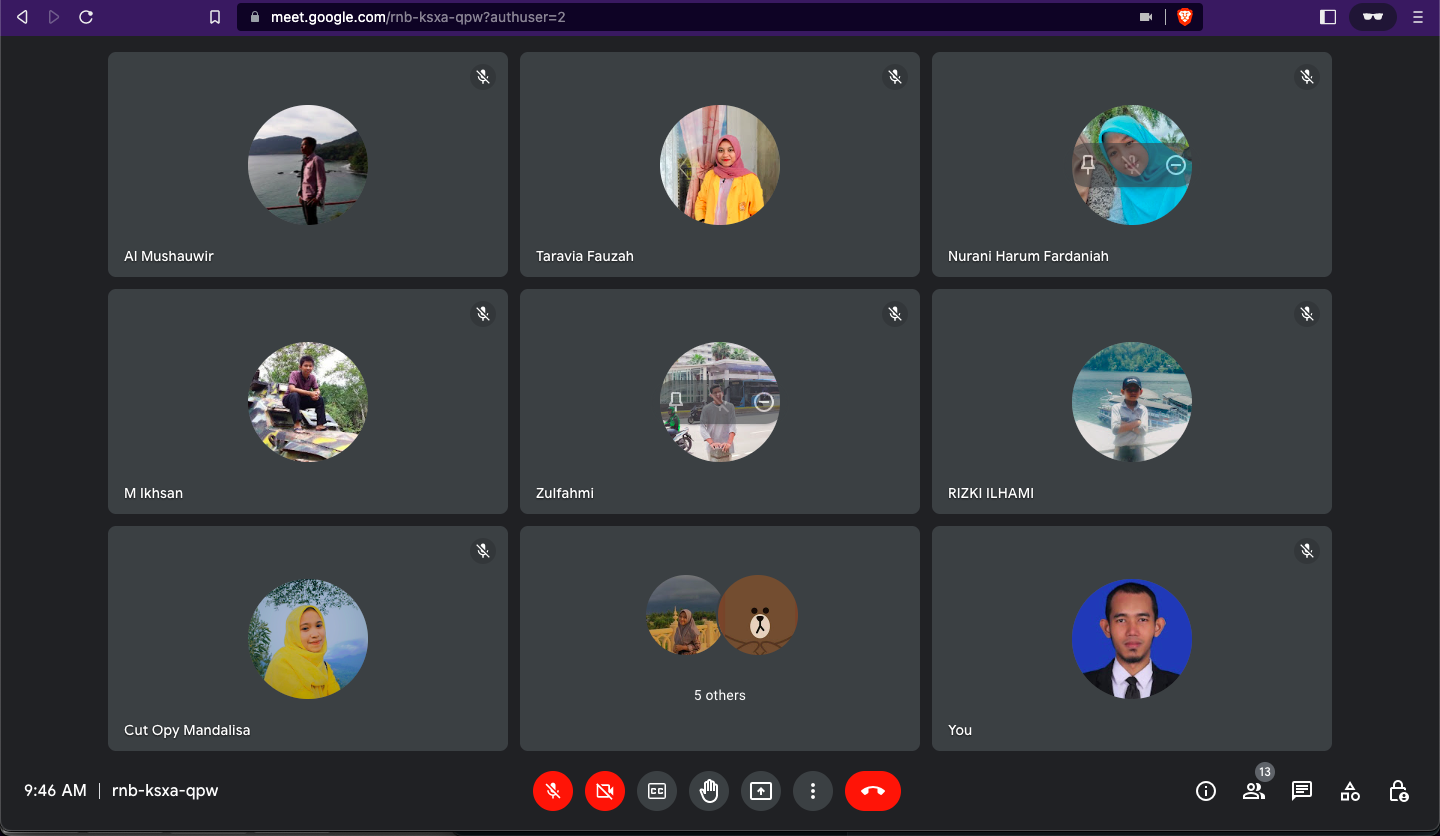
\includegraphics[width=\textwidth]{25-11-2022}
\caption{Perkuliahan Daring via Google Meet}
\label{gam:perkuliahan-25-11}
\end{figure}

\vspace*{-.5cm}
\hrulefill

%%%%%%%%%%%%%%%%%%%%%%%%%%%%%%%%%%%%%%%%%%%%%%%%%%%%%%%%
\clearpage
\newday{\#6 - 1 Desember 2022 menggantikan 13 Oktober 2022
\footnote{Mahasiswa yang hadir:
\begin{enumerate}
\item Adinda Awaliah
\item Arya Saputra $\oplus$
\item Cut Opy Mandalisa
\item Jihan Dwi Sarah
\item M. Ikhsan
\item Muhammad Ikrammullah
\item Muhammad Munawir
\item Nadzura Kumaira
\item Nurani Harum Fardaniah
\item Rauzatinur Syah
\item Resha Russita
\item Rizki Ilhami
\item Salsabila Irmanda
\item Syarfani Akbar
\item Taravia Fauzah
\item Zulfahmi
\end{enumerate}}}

\newthought{Instalasi Apache Hadoop}

Pada pertemuan kedua ini kegiatan yang dilakukan adalah menginstall Apache Hadoop pada \textit{environment} yang telah dibuat pada pertemuan sebelumnya. Untuk menginstall Apache Hadoop dapat mengikut langkah-langkah berikut ini:

\begin{enumerate}
\item Membuat Group dan User Baru
\begin{itemize}
\item Membuat group \\
{\tt sudo addgroup hadoop}
\item Membuat User Baru dan Menambahkan ke Group \\
{\tt sudo adduser -ingroup hadoop hdfs}
\item Ubah Hak Akses \\
{\tt sudo visudo}
\item Tambahkan Kode \\
{\tt hdfs	ALL=(ALL:ALL) ALL}
\item Ganti ke User Baru \\
{\tt su - hdfs}
\end{itemize}

\item Install Java \\
{\tt sudo apt update} \\
{\tt sudo apt install openjdk-8-jdk -y} \\

\item Verifikasi Hasil Instalasi Java \\
{\tt java -version} \\
Jika instalasi java berhasil tanpa ada bug atau error maka akan menampilkan hasil seperti pada Gambar \ref{gam:java-version}.

\begin{figure}
\setlength{\belowcaptionskip}{-10pt}
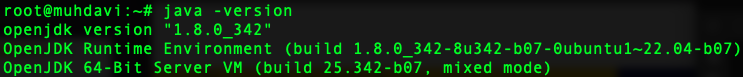
\includegraphics[width=\textwidth]{java-version}
\caption{Versi Java yang Terinstall}
\label{gam:java-version}
\end{figure}

\item Setting SSH \\
\begin{itemize}
\item Uninstall OpenSSH \\
{\tt sudo apt remove openssh-server openssh-client}
\item Install OpenSSH Baru \\
{\tt sudo apt update} \\
{\tt sudo apt install openssh-server openssh-client} \\
{\tt sudo ufw allow 22} \\
{\tt sudo systemctl restart ssh} \\
{\tt sudo apt install ssh} \\
{\tt sudo apt install rsync}
\item Generate Key \\
{\tt ssh-keygen -t dsa -P '' -f $\sim$/.ssh/id\_dsa} \\
{\tt cat $\sim$/.ssh/id\_dsa.pub >> $\sim$/.ssh/authorized\_keys} \\
{\tt ssh-keygen -t rsa}
\item Coba Masuk via SSH \\
{\tt ssh localhost}
\item Jika masih harus memasukkan password, lanjutkan langakh berikut. \\
{\tt ssh-keygen -t rsa} \\
{\tt cat $\sim$/.ssh/id\_rsa.pub >> $\sim$/.ssh/authorized\_keys} \\
{\tt chmod og-wx $\sim$/.ssh/authorized\_keys} \\
{\tt sudo apt-get update}
\item Coba Masuk via SSH Lagi \\
{\tt ssh localhost}
\item Jika sudah berhasil, keluar dengan perintah {\tt exit} \\
{\tt exit}
\end{itemize}

\item Download Apache Hadoop \\
{\tt wget https://dlcdn.apache.org/hadoop/common/hadoop-3.3.4/hadoop-3.3.4.tar.gz}

\item Ekstrak Apache Hadoop \\
{\tt tar -xzvf hadoop-3.3.4.tar.gz }
\begin{itemize}
\item x $\Rightarrow$ ekstrak file arsip.
\item z $\Rightarrow$ filter file arsip melalui gzip.
\item v $\Rightarrow$ menampilkan proses.
\item f $\Rightarrow$ nama file arsip.
\end{itemize}

\item Pindahkan hasil ekstraksi ke {\tt /usr/local/} \\
{\tt sudo mv hadoop-3.3.4 /usr/local/hadoop}

\item Ubah Hak Akses {\tt /usr/local/hadoop} \\
{\tt sudo chown -R hdfs:hadoop /usr/local/hadoop} \\
{\tt sudo chmod -R 777 /usr/local/hadoop}

\item Edit file {\tt sysctl.conf} untuk Disable IPV6
\begin{itemize}
\item Buka file {\tt sysctl.conf} \\
{\tt sudo nano /etc/sysctl.conf}
\item Tambahkan Kode
\begin{lstlisting}
net.ipv6.conf.all.disable_ipv6=1
net.ipv6.conf.lo.disable_ipv6=1
net.ipv6.conf.default_ipv6=1
\end{lstlisting}
\end{itemize}

\item Edit file {\tt hadoop-env.sh} \\
{\tt cd /usr/local/hadoop/etc/hadoop} \\
{\tt sudo nano hadoop-env.sh} \\

\begin{lstlisting}
export JAVA_HOME=/usr/lib/jvm/java-8-openjdk-amd64
export HADOOP_OPTS=-Djava.net.preferIPv4Stack=true
export HADOOP_HOME_WARN_SUPPRESS="TRUE"
export HADOOP_ROOT_LOGGER="WARN"
\end{lstlisting}

\item Menambahkan Hadoop ke {\tt .bashrc} \\
{\tt sudo nano $\sim$/.bashrc} \\
\begin{lstlisting}
#Hadoop Location
export HADOOP_HOME=/usr/local/hadoop
export HADOOP_CONF_DIR=/usr/local/hadoop/etc/hadoop
export HADOOP_MAPRED_HOME=/usr/local/hadoop
export HADOOP_COMMON_HOME=/usr/local/hadoop
export HADOOP_HDFS_HOME=/usr/local/hadoop
export YARN_HOME=/usr/local/hadoop
export PATH=$PATH:/usr/local/hadoop/bin
export PATH=$PATH:/usr/local/hadoop/sbin

#Hadoop Native Location
export HADOOP_COMMON_LIB_NATIVE_DIR=$HADOOP_HOME/lib/native
export HADOOP_OPTS="$HADOOP_OPTS -Djava.library.path=$HADOOP_HOME/lib/native"
export LD_LIBRARY_PATH=$HADOOP_HOME/lib/native
\end{lstlisting}

{\tt source .bashrc}

\item Verifikasi Hasil Instalasi Hadoop \\
{\tt hadoop version} \\
Jika instalasi hadoop berhasil, maka ketika mengecek versi hadoop akan muncul seperti yang diperlihatkan pada Gambar \ref{gam:hadoop-version}.
\begin{figure}[!ht]
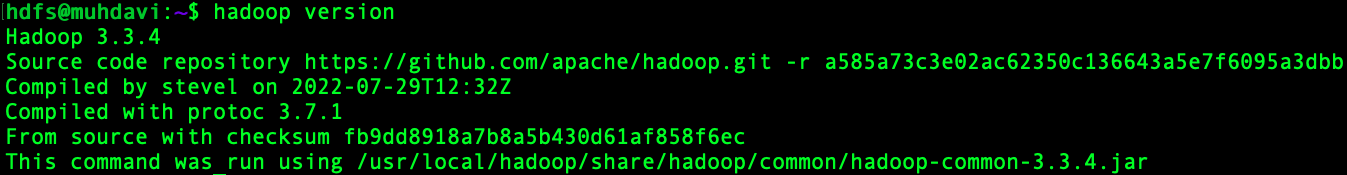
\includegraphics[width=\textwidth]{hadoop-version}
\caption{Versi Hadoop Terinstall 3.3.4}
\label{gam:hadoop-version}
\end{figure}
\end{enumerate}
 
\hrulefill

%%%%%%%%%%%%%%%%%%%%%%%%%%%%%%%%%%%%%%%%%%%%%%%%%%%%%%%%
\clearpage
\newday{\#7 - 2 Desember 2022 menggantikan 20 Oktober 2022
\footnote{Mahasiswa yang hadir:
\begin{enumerate}
\item Muhammad Munawir
\item Rizki Ilhami
\item Rauzatinur Syah
\item Salsabila Irmanda
\item Adjie Yusmunandar
\item Nurani Harum Fardaniah
\item Cut Opy Mandalisa
\item Resha Russita
\item Taravia Fauzah
\item Adinda Awaliah
\item Jihan Dwi Sarah
\item M. Ikhsan
\item Zulfahmi
\end{enumerate}}}

\newthought{Konfigurasi Apache Hadoop}

Setelah selesai meng-install Hadoop, kita perlu konfigurasi beberapa file Hadoop agar memudahkan kita dalam memonitoring ekosistem Hadoop yang telah diinstall.

\begin{enumerate}
\item Konfigurasi File Hadoop \\
Beberapa file Hadoop yang perlu dikonfigurasi berada pada folder {\tt hadoop/etc/hadoop} seperti yang diperlihatkan pada Gambar \ref{gam:file-hadoop}. Konfigurasi file-file tersebut dapat menggunakan {\tt nano} diikuti nama file. Sisipkan kode konfigurasi diantara tag {\tt <configuration> $\cdots$ </configuration>}.

\begin{figure}[!ht]
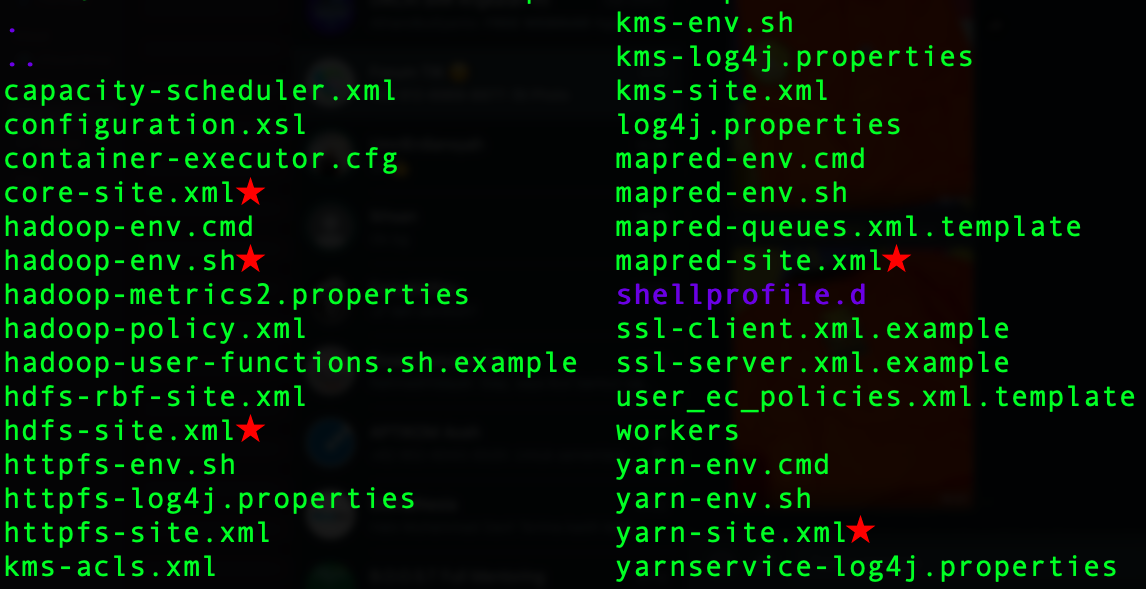
\includegraphics[width=\textwidth]{file-hadoop}
\caption{File Konfigurasi Hadoop}
\label{gam:file-hadoop}
\end{figure}

Berikut bebrapa file yang perlu dikonfigurasi dan lakukan dengan hati-hati serta teliti malalui perintah berikut:

{\tt cd /usr/local/hadoop/etc/hadoop} \\
{\tt sudo nano nama-file}

\begin{itemize}

\item {\tt sudo nano core-site.xml}
\begin{lstlisting}
<property>
	<name>hadoop.tmp.dir</name>
	<value>/app/hadoop/tmp</value>
</property>
<property>
	<name>fs.default.name</name>
	<value>hdfs://localhost:9000</value>
</property>
\end{lstlisting}

\item {\tt sudo nano hdfs-site.xml}
\begin{lstlisting}
<property>
	<name>dfs.replication</name>
	<value>1</value>
</property>
<property>
	<name>dfs.namenode.name.dir</name>
	<value>file:/usr/local/hadoop/yarn_data/hdfs/namenode</value>
</property>
<property>
	<name>dfs.datanode.data.dir</name>
	<value>file:/usr/local/hadoop/yarn_data/hdfs/datanode</value>
</property>
\end{lstlisting}

\item {\tt sudo nano mapred-site.xml}
\begin{lstlisting}
<property>
	<name>mapred.framework.name</name>
	<value>yarn</value>
</property>
<property>
	<name>mapreduce.jobhistory.address</name>
	<value>localhost:10020</value>
</property>
\end{lstlisting}

\item {\tt sudo nano yarn-site.xml}
\begin{lstlisting}
<property>
	<name>yarn.nodemanager.aux-services</name>
	<value>mapreduce_shuffle</value>
</property>
<property>
	<name>yarn.nodemanager.aux-services.mapreduce.shuffle.class</name>
	<value>org.apache.hadoop.mapred.ShuffleHandler</value>
</property>
\end{lstlisting}
\end{itemize}

\item Membuat Folder Sementara (\textit{Temporary}) untuk HDFS \\
{\tt sudo mkdir -p /app/hadoop/tmp} \\
{\tt sudo chmod -R 777 /app/hadoop/tmp} \\
{\tt sudo chown -R hdfs:hadoop /app/hadoop/tmp}

\item Membuat Folder {\tt namenode} dan {\tt datanode} \\
{\tt sudo mkdir -p /usr/local/hadoop/yarn\_data/hdfs/namenode} \\
{\tt sudo mkdir -p /usr/local/hadoop/yarn\_data/hdfs/datanode} \\
{\tt sudo chown -R hdfs:hadoop /usr/local/hadoop/yarn\_data/hdfs/namenode} \\
{\tt sudo chown -R hdfs:hadoop /usr/local/hadoop/yarn\_data/hdfs/datanode} \\
{\tt sudo chmod -R 777 /usr/local/hadoop/yarn\_data/hdfs/namenode} \\
{\tt sudo chmod -R 777 /usr/local/hadoop/yarn\_data/hdfs/datanode}

\item Jalankan Perintah Format HDFS \\
{\tt hdfs namenode -format}

\item Jalankan Hadoop Service \\
{\tt start-dfs.sh} \\
{\tt start-yarn.sh} \\

\item Cek Hadoop Service
\begin{itemize}
\item Jalankan perintah {\tt jps}
\item Akses melalui web browser dengan alamat \url{http://localhost:9870}\footnote{Seperti yang diperlihatkan pada Gambar \ref{gam:namenode}} atau \url{http://localhost:8088}\footnote{Seperti yang diperlihatkan pada Gambar \ref{gam:resourcemanager}}.
\end{itemize}

\begin{figure}[!ht]
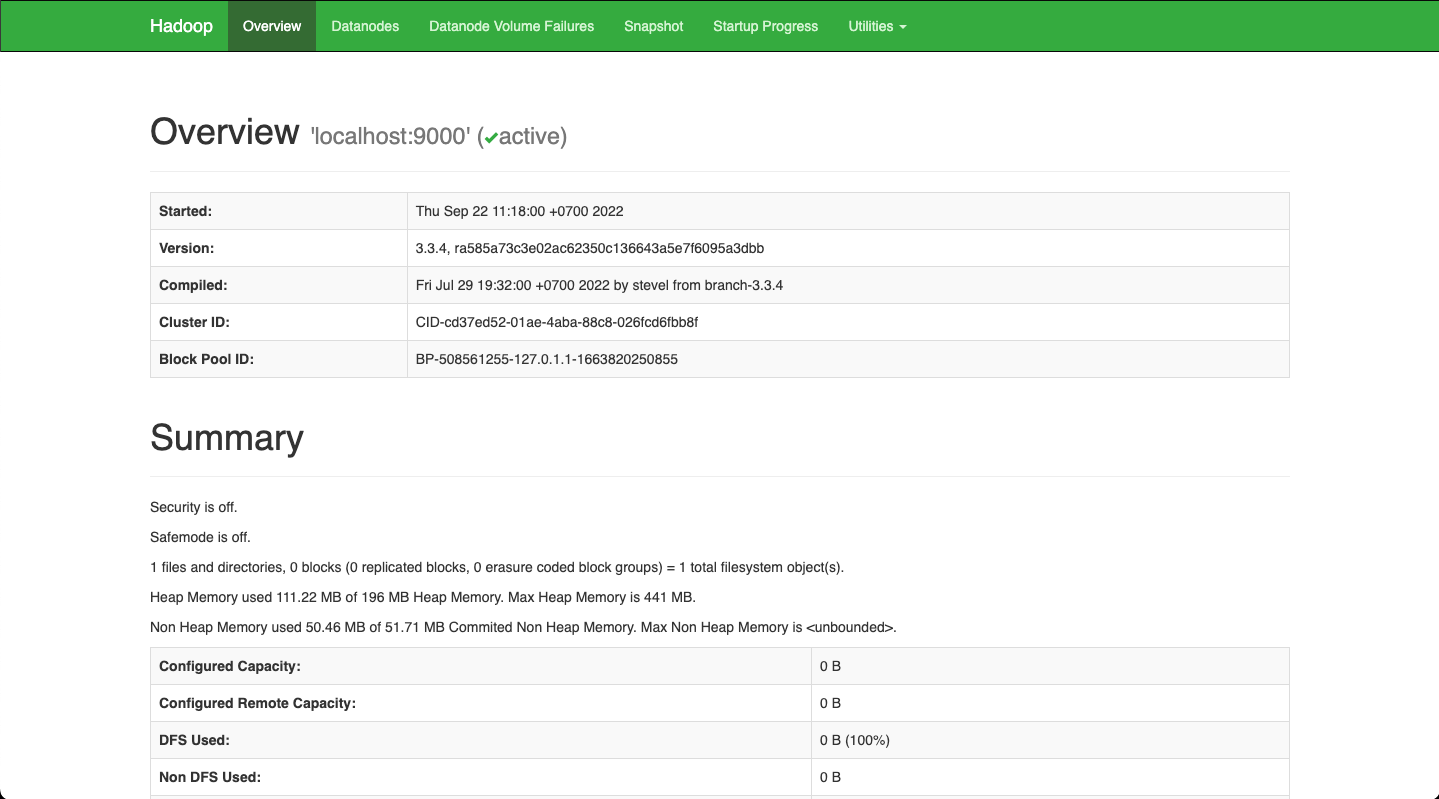
\includegraphics[width=\textwidth]{namenode}
\label{gam:namenode}
\end{figure}
\vspace*{-.7cm}
\begin{figure}[!ht]
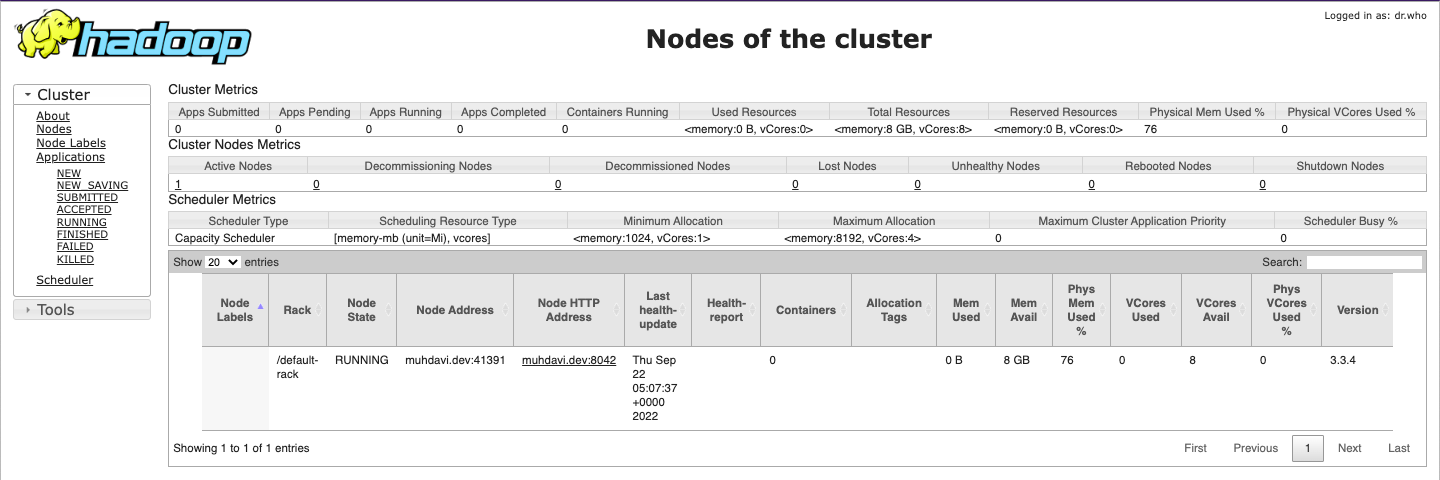
\includegraphics[width=\textwidth]{resourcemanager}
\caption{Resource Manager Hadoop}
\label{gam:resourcemanager}
\end{figure}

\vspace*{-.7cm}
\item Hentikan Hadoop Service
\begin{itemize}
\item Hentikan Service Tertentu \\
{\tt stop-dfs.sh} atau {\tt stop-yarn.sh}
\item Hentikan Semua Service \\
{\tt stop-all.sh}
\end{itemize}
\end{enumerate}
% mounting data shared folder
% sudo mount -t vboxsf share /mnt/share

\vspace*{.1cm}
\hrulefill

%%%%%%%%%%%%%%%%%%%%%%%%%%%%%%%%%%%%%%%%%%%%%%%%%%%%%%%%
\clearpage
\newday{\#8 - 8 Desember 2022 menggantikan 3 November 2022
\footnote{Mahasiswa yang hadir:
\begin{enumerate}
\item Adinda Awaliah
\item Adjie Yusmunandar
%\item Arya Saputra
\item Cut Opy Mandalisa
%\item Faiza Yuwafiqi
\item Jihan Dwi Sarah
\item M. Ikhsan
\item Muhammad Ikrammullah
\item Muhammad Munawir
%\item Nadzura Kumaira
\item Nurani Harum Fardaniah
%\item Nuraula Tafiza
%\item Nurul Aflah
\item Rauzatinur Syah
\item Resha Russita
\item Rizki Ilhami
\item Salsabila Irmanda
%\item Siti Hajar Al Zahra
%\item Syarfani Akbar
\item Taravia Fauzah
\item Zulfahmi
\end{enumerate}}}

\newday{\#9 - 9 Desember 2022 menggantikan 10 November 2022
\footnote{Mahasiswa yang hadir:
\begin{enumerate}
\item Adinda Awaliah
\item Adjie Yusmunandar
%\item Arya Saputra
\item Cut Opy Mandalisa
%\item Faiza Yuwafiqi
\item Jihan Dwi Sarah
\item M. Ikhsan
%\item Muhammad Ikrammullah
\item Muhammad Munawir
%\item Nadzura Kumaira
\item Nurani Harum Fardaniah
%\item Nuraula Tafiza
%\item Nurul Aflah
\item Rauzatinur Syah
\item Resha Russita
\item Rizki Ilhami
\item Salsabila Irmanda
%\item Siti Hajar Al Zahra
%\item Syarfani Akbar
\item Taravia Fauzah
\item Zulfahmi
\end{enumerate}}}

\newthought{Instalasi Apache Hadoop - Lanjutan}

Mahasiswa yang sudah berhasil install Apache Hadoop:
\begin{multicols}{2}
\begin{enumerate}
\item Taravia Fauzah
\item Jihan Dwi Sarah
\item Salsabila Irmanda
\item Rauzatinur Syah
\item Resha Russita
\end{enumerate}
\end{multicols}

Mahasiswa yang sudah ada progress install Apache Hadoop :
\begin{multicols}{2}
\begin{enumerate}
\item Muhammad Ikrammullah
\item Nurani Harum Fardaniah
\item Rizki Ilhami
\item Zulfahmi
\item Cut Opy Mandalisa
\item M. Ikhsan
\item Adjie Yusmunandar
\item Muhammad Munawir
\end{enumerate}
\end{multicols}

\noindent
Berikut mahasiswa yang belum terlihat progress::
\begin{multicols}{2}
\begin{enumerate}
\item Adinda Awaliah
\item Arya Saputra
\item Faiza Yuwafiqi
\item Nadzura Kumaira
\item Nuraula Tafiza
\item Nurul Aflah
\item Siti Hajar Al Zahra
\item Syarfani Akbar
\end{enumerate}
\end{multicols}

\hrulefill








%%%%%%%%%%%%%%%%%%%%%%%%%%%%%%%%%%%%%%%%%%%%%%%%%%%%%%%%
\clearpage
\newday{\#10 - 15 Desember 2022 menggantikan 10 November 2022}

\newthought{Program WordCount bawaan Hadoop}

Jika sudah selesai malakukan instalasi Hadoop, maka dapat mencoba program bawaan Hadoop untuk memahami bagaimana proses dan cara kerja Hadoop dalam memproses data input hingga menghasilkan sebuah output. Salah satu program yang sudah disediakan oleh Hadoop adalah WordCount, yaitu program menghitung jumlah kata dalam data input yang dibarikan. Silahkan ikuti langkah-langkah berikut ini untuk mengetahui cara penggunaan program WordCount.

\begin{enumerate}
\item Jalankan Hadoop Service \\
{\tt start-dfs.sh} \\
{\tt yarn-dfs.sh}

\item Buat folder input di HDFS\\
{\tt hadoop fs -mkdir /input}

\item Buat file baru dengan nama dan data berikut \\
{\tt sudo nano dataWordCount.txt}
\begin{lstlisting}
AdindaAwaliah, SMA_N_1_Lhokseumawe, Cunda
AdjieYusmunandar, SMK_N_1_Lhokseumawe, Paloh_Lada
AryaSaputra
CutOpyMandalisa, SMA_N_1_Syamtalira_Bayu, Bayu
FaizaYuwafiqi
JihanDwiSarah, SMA_N_1_Lhokseumawe, Panggoi
M.Ikhsan, SMK_N_1_Simpang_Kiri, Subulussalam
MuhammadIkrammullah, SMK_N_1_Lhokseumawe, Banda_Sakti
MuhammadMunawir, SMK_N_1_Lhoksukon, Karing_Meurah_Mulia
NadzuraKumaira, SMK_N_2_Lhokseumawe, Keude_Aceh
NuraniHarumFardaniah, SMK_N_1_Lhoksukon, Buket_Hagu
NuraulaTafiza, SMK_N_1_Lhoksukon, Alue_Buket
NurulAflah
RauzatinurSyah, MAS_Misbahul_Ulum, Geudong
ReshaRussita, SMA_N_1_Lhokseumawe, Alue_Awe
RizkiIlhami, SMK_N_1_Lhoksukon, Lapang
SalsabilaIrmanda, MAS_Misbahul_Ulum, Alue_Awe
SitiHajarAlZahra
SyarfaniAkbar
TaraviaFauzah, SMA_N_1_Dewantara, Blang_Naleung_Mameh
Zulfahmi, SMK_N_1_Lhokseumawe, Kuta_Makmur
\end{lstlisting}

\item Pindahkan file dataWordCount.txt ke folder input di HDFS \\
{\tt hadoop fs -put dataWordCount.txt /input}

\item Jalankan program WordCount \\
{\tt hadoop jar /usr/local/hadoop/share/hadoop/mapreduce/hadoop-mapreduce-examples-3.3.4.jar wordcount /input/dataWordCount.txt /output}
%hadoop jar /usr/local/hadoop/share/hadoop/mapreduce/hadoop-mapreduce-examples-3.2.0.jar wordcount /input/ /output2 -> untuk semua file dari folder input

\item Cek Hasil \\
{\tt hadoop fs -ls /output}

\item Lihat Hasil \\
{\tt hadoop fs -cat /output/part-r-00000}
\end{enumerate}

\newthought{Tugas Praktikum} \\
Screenshot hasil dari langkah 6 dan 7 dan masukkan ke dalam laporan. Kumpulkan melalui {\tt pull requests} dengan format pesan "\textit{Laporan dd-mm-yyyy an. Nama}".

\noindent
Mahasiswa yang sudah berhasil:
\begin{multicols}{2}
\begin{enumerate}
\item Taravia Fauzah
\end{enumerate}
\end{multicols}

\hrulefill

%%%%%%%%%%%%%%%%%%%%%%%%%%%%%%%%%%%%%%%%%%%%%%%%%%%%%%%%
\clearpage
\newday{\#11 - 16 Desember 2022 menggantikan 17 November 2022}

\newthought{Program WordCount dengan Java}

Pada pertemuan sebelumnya telah mencoba program WordCount bawaan Hadoop. Jika dengan program bawaan Hadoop sudah dapat mendapatkan hasil, artinya Hadoop kita sudah bisa digunakan untuk menjalankan program. Ikuti beberapa langkah berikut untuk memberikan pemahaman bagaimana proses membuat program, menyiapkan data, meng-compile program hingga menjalankan program dan memperoleh hasilnya.

\begin{enumerate}
\item Pastikan Hadoop Service sudah berjalan
\item Pastikan data input pada pertemuan sebelumnya masih tersedia di HDFS
\item Buat file baru dengan nama dan kode berikut \\

{\tt sudo nano WordCount.java}
\begin{lstlisting}
import java.io.IOException;
import java.util.StringTokenizer;

import org.apache.hadoop.conf.Configuration;
import org.apache.hadoop.fs.Path;
import org.apache.hadoop.io.IntWritable;
import org.apache.hadoop.io.Text;
import org.apache.hadoop.mapreduce.Job;
import org.apache.hadoop.mapreduce.Mapper;
import org.apache.hadoop.mapreduce.Reducer;
import org.apache.hadoop.mapreduce.lib.input.FileInputFormat;
import org.apache.hadoop.mapreduce.lib.output.FileOutputFormat;

public class WordCount {

    public static class TokenizerMapper
            extends Mapper<Object, Text, Text, IntWritable> {

        private final static IntWritable one = new IntWritable(1);
        private Text word = new Text();

        public void map(Object key, Text value, Context context
        ) throws IOException, InterruptedException {
            StringTokenizer itr = new StringTokenizer(value.toString());
            while (itr.hasMoreTokens()) {
                word.set(itr.nextToken());
                context.write(word, one);
            }
        }
    }

    public static class IntSumReducer
            extends Reducer<Text, IntWritable, Text, IntWritable> {
        private IntWritable result = new IntWritable();

        public void reduce(Text key, Iterable<IntWritable> values,
                           Context context
        ) throws IOException, InterruptedException {
            int sum = 0;
            for (IntWritable val : values) {
                sum += val.get();
            }
            result.set(sum);
            context.write(key, result);
        }
    }

    public static void main(String[] args) throws Exception {
        Configuration conf = new Configuration();
        Job job = Job.getInstance(conf, "word count");
        job.setJarByClass(WordCount.class);
        job.setMapperClass(TokenizerMapper.class);
        job.setCombinerClass(IntSumReducer.class);
        job.setReducerClass(IntSumReducer.class);
        job.setOutputKeyClass(Text.class);
        job.setOutputValueClass(IntWritable.class);
        FileInputFormat.addInputPath(job, new Path(args[0]));
        FileOutputFormat.setOutputPath(job, new Path(args[1]));
        System.exit(job.waitForCompletion(true) ? 0 : 1);
    }
}
\end{lstlisting}
% https://github.com/muhdavi/kode-practice-big-data/blob/main/WordCountJava/src/main/java/WordCount.java

\item Buat classpath \\
{\tt export HADOOP\_CLASSPATH=\$(\$HADOOP\_HOME/bin/hadoop classpath)}

\item Buat folder baru untuk menampung hasil \textit{compile} program java dan ubah hak aksesnya \\
{\tt sudo mkdir JavaCompiled} \\
{\tt sudo chmod -R 777 JavaCompiled}

\item Compile file WordCount.java \\
{\tt \small{javac -classpath \$HADOOP\_CLASSPATH -d JavaCompiled/WordCount.java}}

\item Mengubah file menjadi executable .jar \\
{\tt jar -cvf WordCount.jar -C JavaCompiled/ .}

\item Jalankan program WordCount \\
{\tt hadoop jar WordCount.jar WordCount /input/dataWordCount.txt /ResultWordCountJava}

\item Cek Hasil \\
{\tt hadoop fs -ls /ResultWordCountJava}

\item Lihat Hasil \\
{\tt hadoop fs -cat /ResultWordCountJava/part-r-00000}
\end{enumerate}

\newthought{Tugas Praktikum} \\
Screenshot hasil dari langkah 9 dan 10 serta masukkan ke dalam laporan. Kumpulkan melalui {\tt pull requests} dengan format pesan "\textit{Laporan dd-mm-yyyy an. Nama}".

\noindent
Mahasiswa yang sudah berhasil:
\begin{multicols}{2}
\begin{enumerate}
\item Taravia Fauzah
\end{enumerate}
\end{multicols}

\hrulefill

\begin{comment}
%%%%%%%%%%%%%%%%%%%%%%%%%%%%%%%%%%%%%%%%%%%%%%%%%%%%%%%%
\clearpage
\newday{\#10 - 15 Desember 2022 menggantikan 10 November 2022
\footnote{Mahasiswa yang hadir:
\begin{enumerate}
\item Adinda Awaliah
\item Adjie Yusmunandar
%\item Arya Saputra
\item Cut Opy Mandalisa
%\item Faiza Yuwafiqi
\item Jihan Dwi Sarah
\item M. Ikhsan
%\item Muhammad Ikrammullah
\item Muhammad Munawir
%\item Nadzura Kumaira
\item Nurani Harum Fardaniah
%\item Nuraula Tafiza
%\item Nurul Aflah
\item Rauzatinur Syah
\item Resha Russita
\item Rizki Ilhami
\item Salsabila Irmanda
%\item Siti Hajar Al Zahra
%\item Syarfani Akbar
\item Taravia Fauzah
\item Zulfahmi
\end{enumerate}}}
\newday{\#11 - 16 Desember 2022 menggantikan 17 November 2022
\footnote{Mahasiswa yang hadir:
\begin{enumerate}
\item Adinda Awaliah
\item Adjie Yusmunandar
%\item Arya Saputra
\item Cut Opy Mandalisa
%\item Faiza Yuwafiqi
\item Jihan Dwi Sarah
\item M. Ikhsan
%\item Muhammad Ikrammullah
\item Muhammad Munawir
%\item Nadzura Kumaira
\item Nurani Harum Fardaniah
%\item Nuraula Tafiza
%\item Nurul Aflah
\item Rauzatinur Syah
\item Resha Russita
\item Rizki Ilhami
\item Salsabila Irmanda
%\item Siti Hajar Al Zahra
%\item Syarfani Akbar
\item Taravia Fauzah
\item Zulfahmi
\end{enumerate}}}

\newthought{Program WordCount bawaan Hadoop - Lanjutan}

Mahasiswa yang sudah berhasil install Apache Hadoop:
\begin{multicols}{2}
\begin{enumerate}
\item Taravia Fauzah
\item Jihan Dwi Sarah
\item Salsabila Irmanda
\item Rauzatinur Syah
\item Resha Russita
\end{enumerate}
\end{multicols}

Mahasiswa yang sudah ada progress install Apache Hadoop :
\begin{multicols}{2}
\begin{enumerate}
\item Muhammad Ikrammullah
\item Nurani Harum Fardaniah
\item Rizki Ilhami
\item Zulfahmi
\item Cut Opy Mandalisa
\item M. Ikhsan
\item Adjie Yusmunandar
\item Muhammad Munawir
\end{enumerate}
\end{multicols}

\noindent
Berikut mahasiswa yang belum terlihat progress::
\begin{multicols}{2}
\begin{enumerate}
\item Adinda Awaliah
\item Arya Saputra
\item Faiza Yuwafiqi
\item Nadzura Kumaira
\item Nuraula Tafiza
\item Nurul Aflah
\item Siti Hajar Al Zahra
\item Syarfani Akbar
\end{enumerate}
\end{multicols}

\hrulefill

%%%%%%%%%%%%%%%%%%%%%%%%%%%%%%%%%%%%%%%%%%%%%%%%%%%%%%%%
\clearpage
\newday{\#10 - 15 Desember 2022 menggantikan 10 November 2022}

\newthought{Program WordCount dengan Python}

\begin{enumerate}
\item Pastikan Hadoop Service dan Spark Service berjalan
\item Pastikan data input pada pertemuan sebelumnya masih tersedia di HDFS
\item Buat folder baru untuk menyimpan file Python \\
{\tt sudo mkdir WordCountPython}
\item Buat file baru dengan nama dan kode berikut
\begin{itemize}
\item {\tt map.py} \\
{\tt sudo nano WordCountPython/map.py}
\begin{lstlisting}
#!/usr/bin/env python

import sys

for line in sys.stdin:
    line = line.strip()
    words = line.split()
    for word in words:
        print('{}\t{}'.format(word, 1))
\end{lstlisting}
{\tt wget https://raw.githubusercontent.com/muhdavi/kode-practice- big-data/main/WordCountPython/map.py}

\item {\tt reduce.py} \\
{\tt sudo nano WordCountPython/reduce.py}
\begin{lstlisting}
#!/usr/bin/env python

import sys

current_word = None
current_count = 0
word = None

for line in sys.stdin:
    line = line.strip()
    word, count = line.split('\t', 1)

    try:
        count = int(count)
    except ValueError:
        continue

    if current_word == word:
        current_count += count
    else:
        if current_word:
            print('{}\t{}'.format(current_word, current_count))
        current_count = count

if current_word == word:
    print('{}\t{}'.format(current_word, current_count))
\end{lstlisting}
{\tt wget https://raw.githubusercontent.com/muhdavi/kode-practice- big-data/main/WordCountPython/reduce.py}
\end{itemize}

\item Ubah Hak Akses \\
{\tt sudo chmod +x -R WordCountPython/} 

\item Mencoba Program di Local
\begin{itemize}
\item Mencoba jalankan {\tt map.py} \\
{\tt echo jangan heran jika orang cantik merasa jelek sementara orang jelek merasa cantik | WordCountPython/map.py}
\item Mencoba jalankan {\tt reduce.py} \\
{\tt echo jangan heran jika orang cantik merasa jelek sementara orang jelek merasa cantik | WordCountPython/reduce.py}
\item Mencoba jalankan {\tt map.py} dan {\tt reduce.py}
{\tt echo jangan heran jika orang cantik merasa jelek sementara orang jelek merasa cantik | WordCountPython/map.py | sort | WordCountPython/reduce.py}
\end{itemize}

\item Jalankan Program menggunakan Hadoop \\
{\tt hadoop jar /usr/local/hadoop/share/hadoop/tools/lib/hadoop-streaming-3.3.4.jar -mapper ~/WordCountPython/Map.py -reducer ~/WordCountPython/Reduce.py -input /input/inputWordCount.txt -output /ResultWordCountPython}

\item Cek Hasil \\
{\tt hadoop fs -ls /ResultWordCountPython}

\item Lihat Hasil \\
{\tt hadoop fs -cat /ResultWordCountPython/part-r-00000}
\end{enumerate}

\vspace*{-.5cm}
\newthought{Tugas Praktikum} \\
Screenshot hasil dari langkah 8 dan 9 serta masukkan ke dalam laporan.

\hrulefill

%%%%%%%%%%%%%%%%%%%%%%%%%%%%%%%%%%%%%%%%%%%%%%%%%%%%%%%%
\clearpage
\newday{\#11 - 16 Desember 2022 menggantikan 17 November 2022}

\newthought{Instalasi Apache Spark (PySpark)}

\begin{enumerate}
\item Download Apache Spark \\
{\tt wget https://dlcdn.apache.org/spark/spark-3.3.1/spark-3.3.1-bin-hadoop3.tgz}

\item Ekstrak Apache Spark \\
{\tt tar -xzf spark-3.3.1-bin-hadoop3.tgz /usr/local/spark}

\item Pindahkan hasil ekstraksi ke {\tt /usr/local/} \\
{\tt sudo mv spark-3.3.1-bin-hadoop3 /usr/local/spark}

\item Menambahkan Spark ke {\tt .bashrc} \\
{\tt sudo nano $\sim$/.bashrc}
\begin{lstlisting}
#Spark Location
export SPARK_HOME=/usr/local/spark
export PATH=$PATH:$SPARK_HOME/bin:$SPARK_HOME/sbin
\end{lstlisting}
{\tt source $\sim$/.bashrc}

\item Verifikasi Hasil Instalasi Spark

\begin{figure}[!ht]
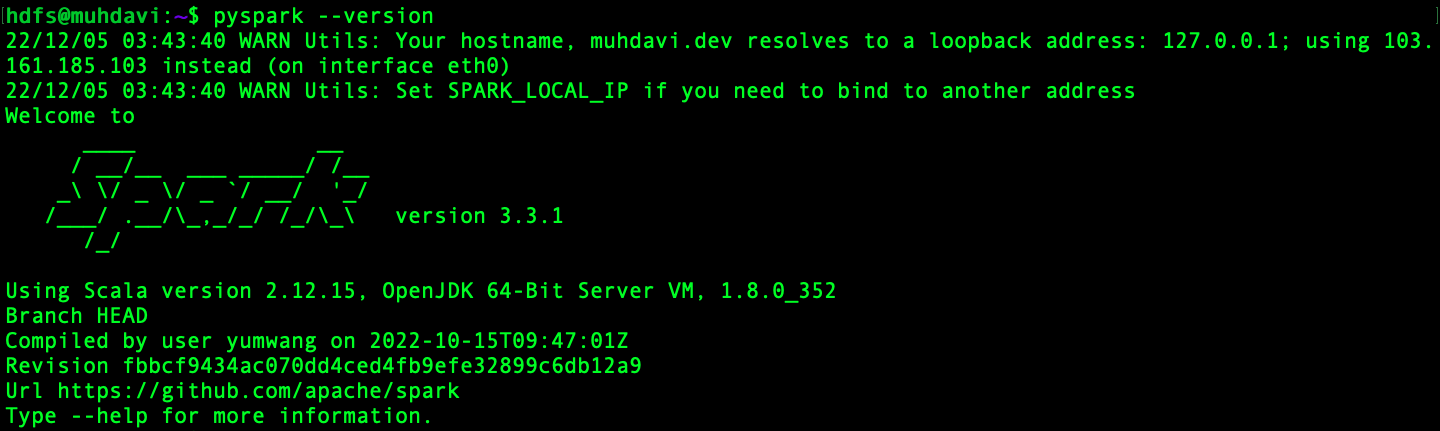
\includegraphics[width=\textwidth]{spark-version}
\caption{Versi Spark Terinstall 3.3.1 }
\label{gam:form-ssh}
\end{figure}

\item Jalankan Spark Service \\
{\tt start-master.sh}

\item Hentikan Spark Service \\
{\tt stop-master.sh}
\end{enumerate}

\newthought{Tugas Praktikum} \\
Screenshot hasil dari langkah 5 dan masukkan ke dalam laporan.

\hrulefill

%%%%%%%%%%%%%%%%%%%%%%%%%%%%%%%%%%%%%%%%%%%%%%%%%%%%%%%%
\clearpage
\newday{\#12 - 22 Desember 2022 menggantikan 24 November 2022}

\newthought{Pertemuan 11}

\hrulefill

%%%%%%%%%%%%%%%%%%%%%%%%%%%%%%%%%%%%%%%%%%%%%%%%%%%%%%%%
\clearpage
\newday{\#13 - 23 Desember 2022 menggantikan 1 Desember 2022}

\newthought{Pertemuan 12}

\hrulefill

%%%%%%%%%%%%%%%%%%%%%%%%%%%%%%%%%%%%%%%%%%%%%%%%%%%%%%%%
\clearpage
\newday{\#14 - 29 Desember 2022 menggantikan 8 Desember 2022}

\newthought{Pertemuan 13}

\hrulefill

%%%%%%%%%%%%%%%%%%%%%%%%%%%%%%%%%%%%%%%%%%%%%%%%%%%%%%%%
\clearpage
\newday{\#15 - 30 Desember 2022 menggantikan 15 Desember 2022}

\newthought{Pertemuan 14}

\hrulefill

%%%%%%%%%%%%%%%%%%%%%%%%%%%%%%%%%%%%%%%%%%%%%%%%%%%%%%%%
\clearpage
\newday{\#16 - 30 Desember 2022 menggantikan 22 Desember 2022}

\newthought{Pertemuan 15}

\hrulefill
\end{comment}

%%%%%%%%%%%%%%%%%%%%%%%%%%%%%%%%%%%%%%%%%%%%%%%%%%%%%%%%

\newthought{\textbf{Adinda Awaliah - 2020903430004 - TRKJ 3B}}

\newday{\textbf{15 september 2022}}
\begin{enumerate}
\item Kendala dan Solusi
% jelaskan kendala dan penyebab yang dialami saat mengikuti praktikum serta solusi atau langkah-langkah yang telah dilakukan
\newline praktikum instalasi apache hadoop tidak ada kendala.

\item Kesimpulan
% berikan kesimpulan dari praktikum yang telah dikerjkan
\newline berhasil melakukan instalasi.

\begin{figure}
\setlength{\belowcaptionskip}{-10pt}
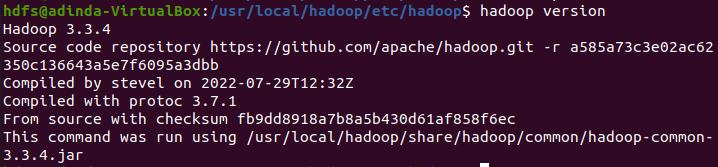
\includegraphics[width=\textwidth]{AdindaAwaliah/hasil instalasi apache hadoop}
\caption{Versi Java yang Terinstall}
\label{gam:hasil instalasi apache hadoop}
\end{figure}

\end{enumerate}

\newday{\textbf{1 desember 2022}}
\begin{enumerate}
\item Kendala dan Solusi
% jelaskan kendala dan penyebab yang dialami saat mengikuti praktikum serta solusi atau langkah-langkah yang telah dilakukan

\item Kesimpulan
% berikan kesimpulan dari praktikum yang telah dikerjkan

\end{enumerate}

\newday{\textbf{02 desember 2022}}
\begin{enumerate}
\item Kendala dan Solusi
% jelaskan kendala dan penyebab yang dialami saat mengikuti praktikum serta solusi atau langkah-langkah yang telah dilakukan

\item Kesimpulan
% berikan kesimpulan dari praktikum yang telah dikerjkan

\end{enumerate}

\newday{\textbf{08 desember 2022}}
\begin{enumerate}
\item Kendala dan Solusi
% jelaskan kendala dan penyebab yang dialami saat mengikuti praktikum serta solusi atau langkah-langkah yang telah dilakukan

\item Kesimpulan
% berikan kesimpulan dari praktikum yang telah dikerjkan

\end{enumerate}

\newday{\textbf{09 desember 2022}}
\begin{enumerate}
\item Kendala dan Solusi
% jelaskan kendala dan penyebab yang dialami saat mengikuti praktikum serta solusi atau langkah-langkah yang telah dilakukan

\item Kesimpulan
% berikan kesimpulan dari praktikum yang telah dikerjkan

\end{enumerate}

\newday{\textbf{15 desember 2022}}
\begin{enumerate}
\item Kendala dan Solusi
% jelaskan kendala dan penyebab yang dialami saat mengikuti praktikum serta solusi atau langkah-langkah yang telah dilakukan

\item Kesimpulan
% berikan kesimpulan dari praktikum yang telah dikerjkan

\end{enumerate}

\newday{\textbf{16 desember 2022}}
\begin{enumerate}
\item Kendala dan Solusi
% jelaskan kendala dan penyebab yang dialami saat mengikuti praktikum serta solusi atau langkah-langkah yang telah dilakukan

\item Kesimpulan
% berikan kesimpulan dari praktikum yang telah dikerjkan

\end{enumerate}

\newday{\textbf{22 desember 2022}}
\begin{enumerate}
\item Kendala dan Solusi
% jelaskan kendala dan penyebab yang dialami saat mengikuti praktikum serta solusi atau langkah-langkah yang telah dilakukan

\item Kesimpulan
% berikan kesimpulan dari praktikum yang telah dikerjkan

\end{enumerate}

\newday{\textbf{23 desember 2022}}
\begin{enumerate}
\item Kendala dan Solusi
% jelaskan kendala dan penyebab yang dialami saat mengikuti praktikum serta solusi atau langkah-langkah yang telah dilakukan

\item Kesimpulan
% berikan kesimpulan dari praktikum yang telah dikerjkan

\end{enumerate}

\newthought{\textbf{Adjie Yusmunandar - 2020903430005 - TRKJ 3B}}

\newday{\textbf{22 September 2022}}
\begin{enumerate}
\item Kendala dan Solusi
% jelaskan kendala dan penyebab yang dialami saat mengikuti praktikum serta solusi atau langkah-langkah yang telah dilakukan

\item Kesimpulan
% berikan kesimpulan dari praktikum yang telah dikerjkan

\end{enumerate}

\newday{\textbf{1 Desember 2022}}
\begin{enumerate}
\item Kendala dan Solusi
% jelaskan kendala dan penyebab yang dialami saat mengikuti praktikum serta solusi atau langkah-langkah yang telah dilakukan

\item Kesimpulan
% berikan kesimpulan dari praktikum yang telah dikerjkan

\end{enumerate}

\newday{\textbf{2 Desember 2022}}
\begin{enumerate}
\item Kendala dan Solusi
% jelaskan kendala dan penyebab yang dialami saat mengikuti praktikum serta solusi atau langkah-langkah yang telah dilakukan

\item Kesimpulan
% berikan kesimpulan dari praktikum yang telah dikerjkan

\end{enumerate}

\newday{\textbf{8 Desember 2022}}
\begin{enumerate}
\item Kendala dan Solusi
% jelaskan kendala dan penyebab yang dialami saat mengikuti praktikum serta solusi atau langkah-langkah yang telah dilakukan

\item Kesimpulan
% berikan kesimpulan dari praktikum yang telah dikerjkan

\end{enumerate}


\newthought{\textbf{Adinda Awaliah - 2020903430004 - TRKJ 3B}}

\newday{\textbf{22 September 2022}}
\begin{enumerate}
\item Kendala dan Solusi
% jelaskan kendala dan penyebab yang dialami saat mengikuti praktikum serta solusi atau langkah-langkah yang telah dilakukan

\item Kesimpulan
% berikan kesimpulan dari praktikum yang telah dikerjkan

\end{enumerate}


\newthought{\textbf{Cut Opy Mandalisa - 2020903430012 - TRKJ 3B}}

\newday{\textbf{1-2 Desember 2022- Instalasi dan Konfigurasi Hadoop}}
\begin{enumerate}
\item Kendala dan Solusi\\
% jelaskan kendala dan penyebab yang dialami saat mengikuti praktikum serta solusi atau langkah-langkah yang telah dilakukan
Pada Praktikum pertama yaitu penginstalan apache hadoop.kendala yang didapat tidak bisa membuka firefox kemudian solusinya dengan menginstal firefox baru.

\begin{figure}[!ht]
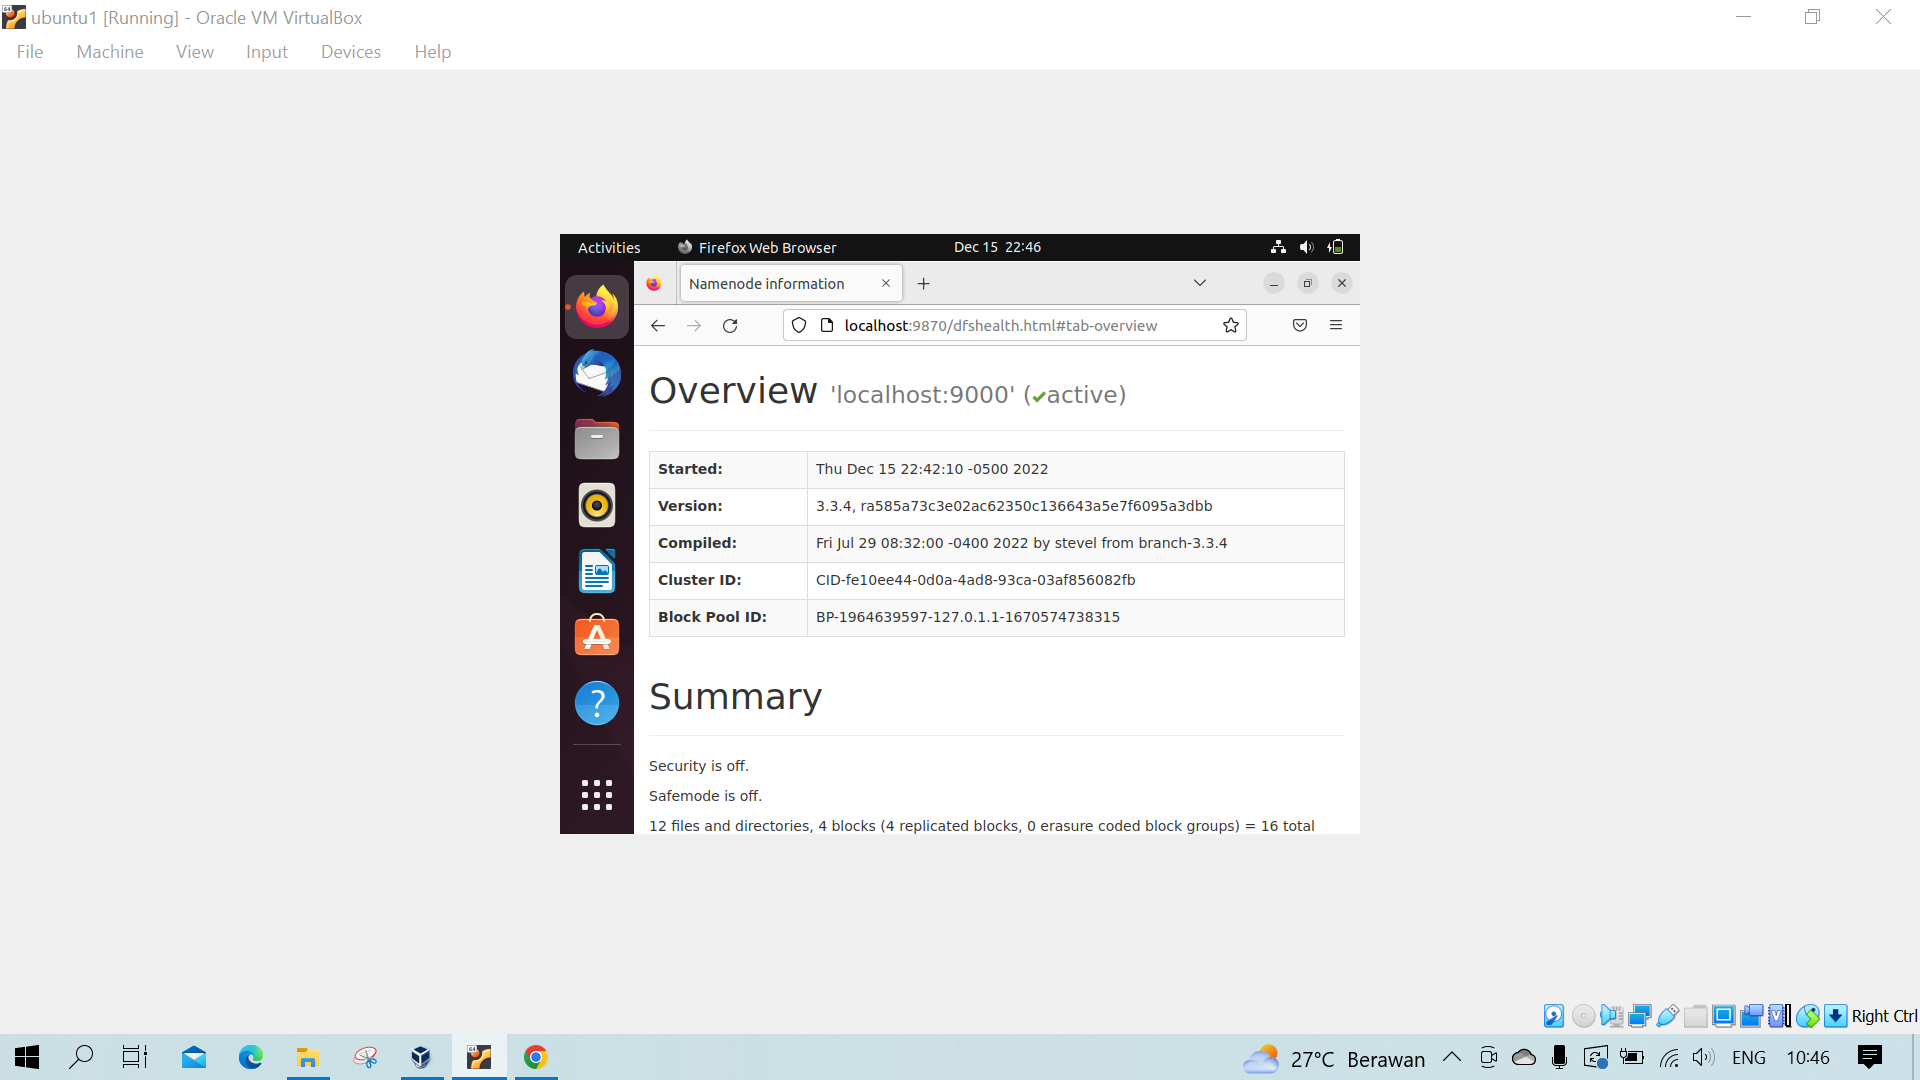
\includegraphics[width=\textwidth]{CutOpyMandalisa/01}
\caption{hasil dari cek hadoop service}
\label{gam:perkuliahan-25-11}
\end{figure}

\begin{figure}[!ht]
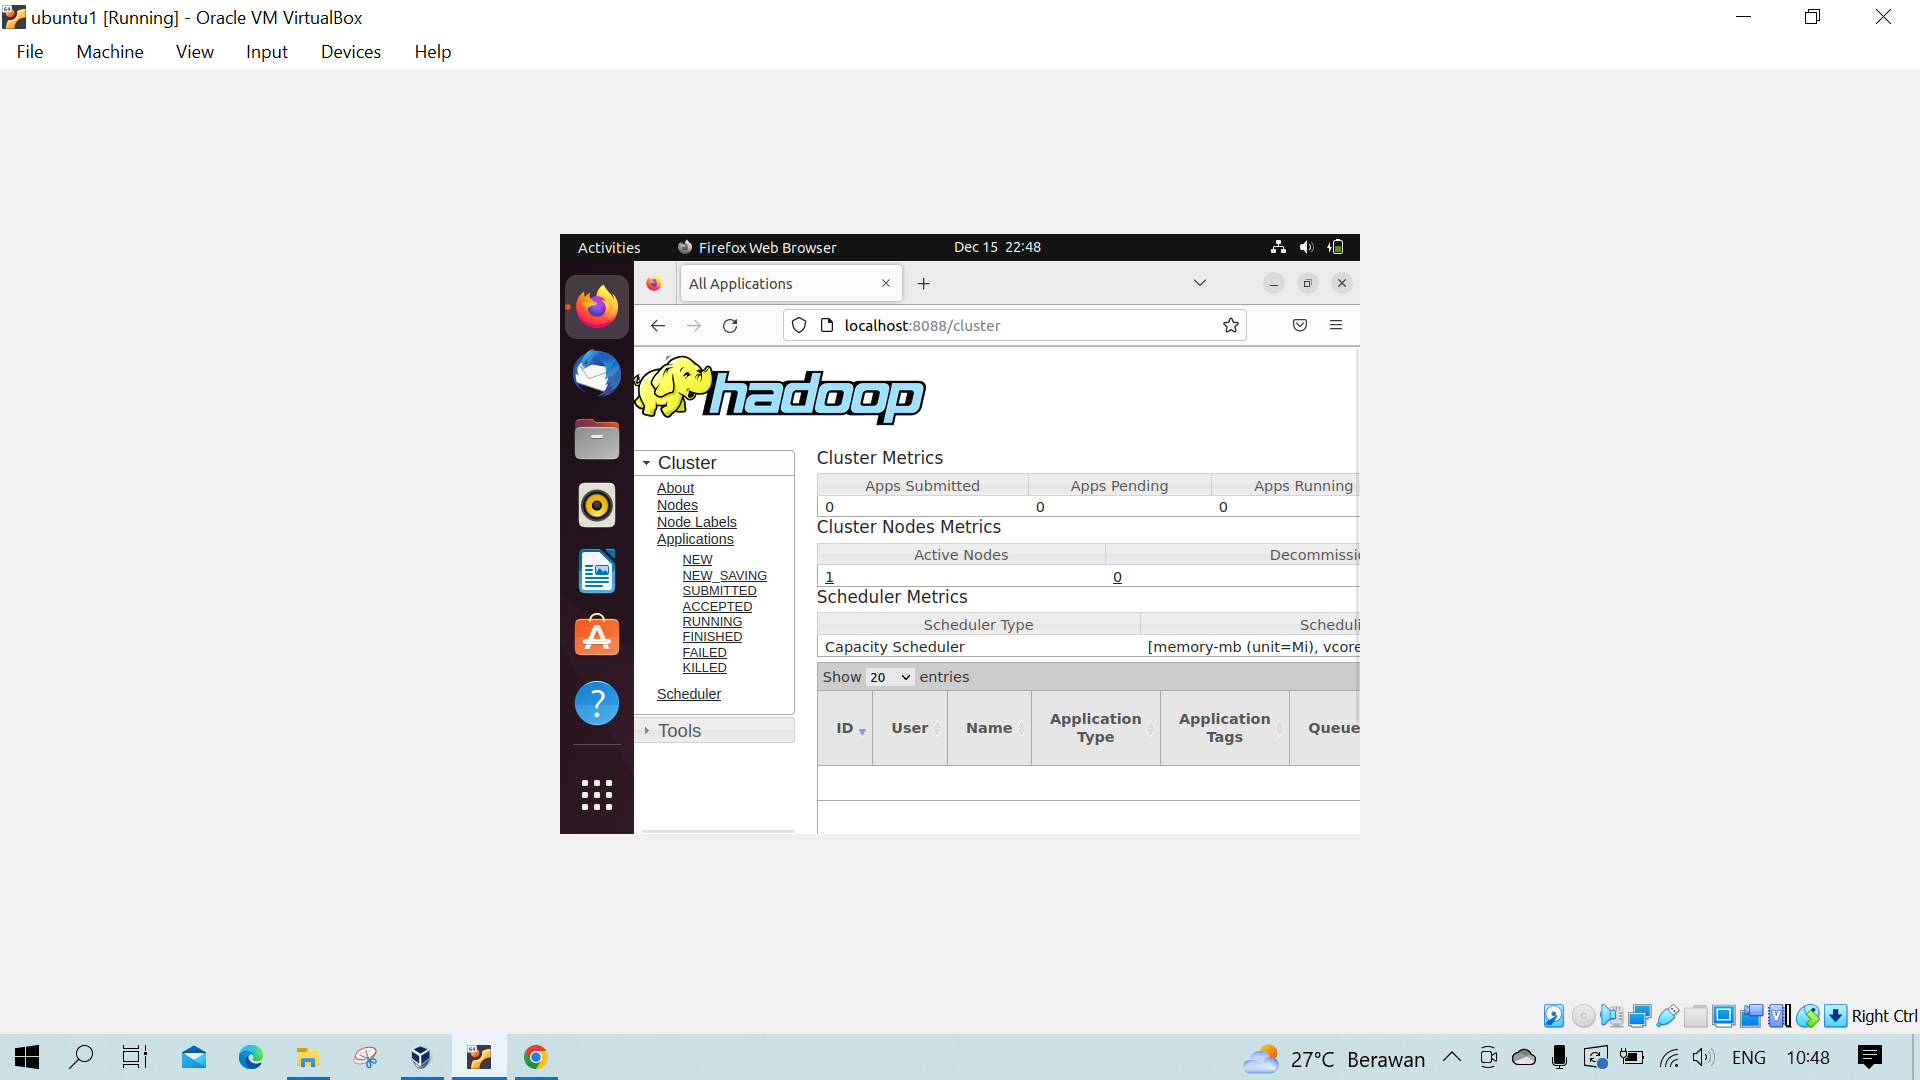
\includegraphics[width=\textwidth]{CutOpyMandalisa/02}
\caption{hasil cek hadoop service}
\label{gam:perkuliahan-25-11}
\end{figure}

\item Kesimpulan\\
% berikan kesimpulan dari praktikum yang telah dikerjkan
Behasil mendownload dan menginstal Apache hadoop dan sudah bisa dijalankan
\end{enumerate}


\newday{\textbf{08 Desember 2022-WordCount bawaan Hadoop}}
\begin{enumerate}

\item Kendala dan Solusi
\newpage
% jelaskan kendala dan penyebab yang dialami saat mengikuti praktikum serta solusi atau langkah-langkah yang telah dilakukan
Pada praktikum ini membuat program WordCount bawaan Hadoop. Pada melakukan praktikum tidak ada kendala hanya erorr dikarenakan salah memasukkan perintah.

\begin{figure}[!ht]
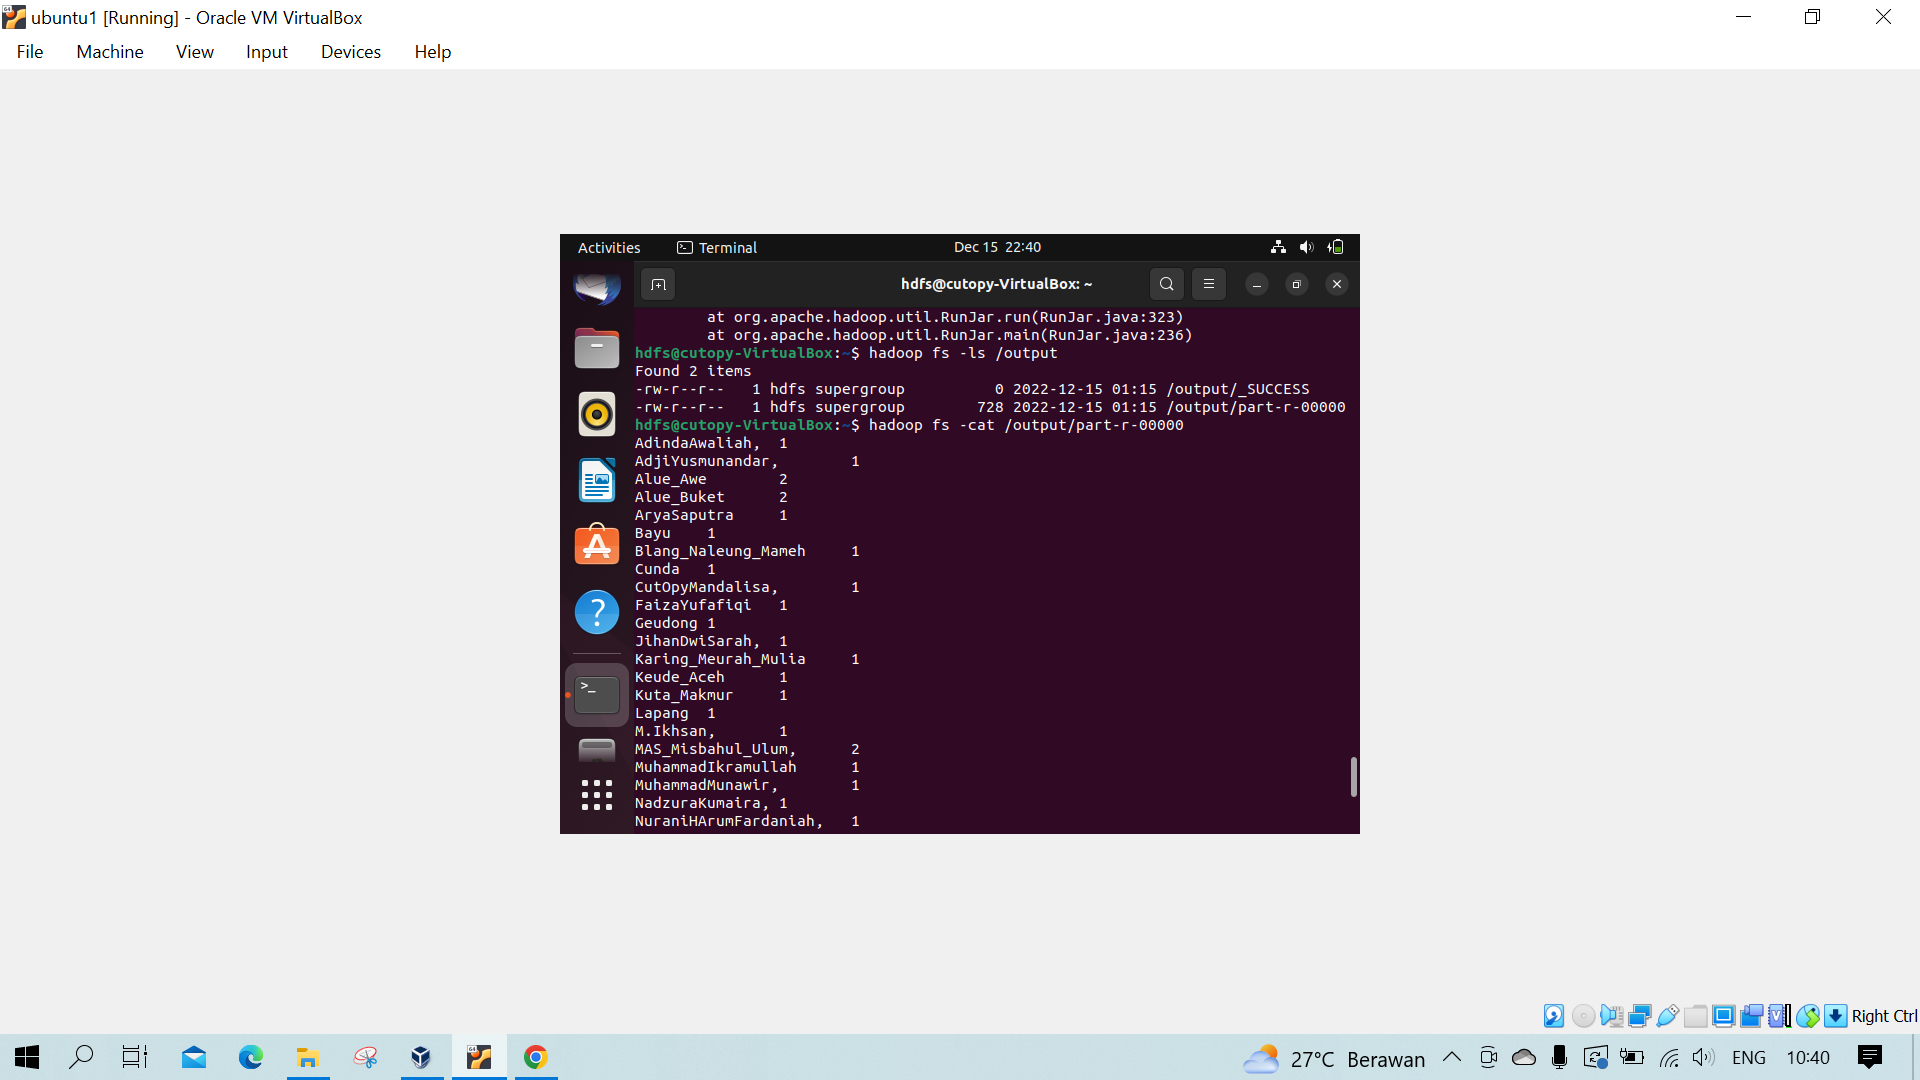
\includegraphics[width=\textwidth]{CutOpyMandalisa/03}
\caption{hasil WordCount bawaan Hadoop}
\label{gam:perkuliahan-25-11}
\end{figure}

\item Kesimpulan\\
% berikan kesimpulan dari praktikum yang telah dikerjkan
Pada praktikum ini untuk memahami proses cara kerja pada hadoop dalam memproses data input sehingga menghasilkan output.Wordcount merupakan program untuk menghitung jumlah kata dalam input.
\end{enumerate}


\newday{\textbf{09 Desember 2022-WordCount dengan Java}}
\begin{enumerate}
\item Kendala dan Solusi\\
% jelaskan kendala dan penyebab yang dialami saat mengikuti praktikum serta solusi atau langkah-langkah yang telah dilakukan
Pada praktikum ini membuat program WordCount dengan java.Pada saat melakukan praktikum terdapat error akan tetapi erorrnya disebabkan salah memasukkan perintah codingannya.solusinya harus lebih teliti saat memasukkan codingan tersebut.

\begin{figure}[!ht]
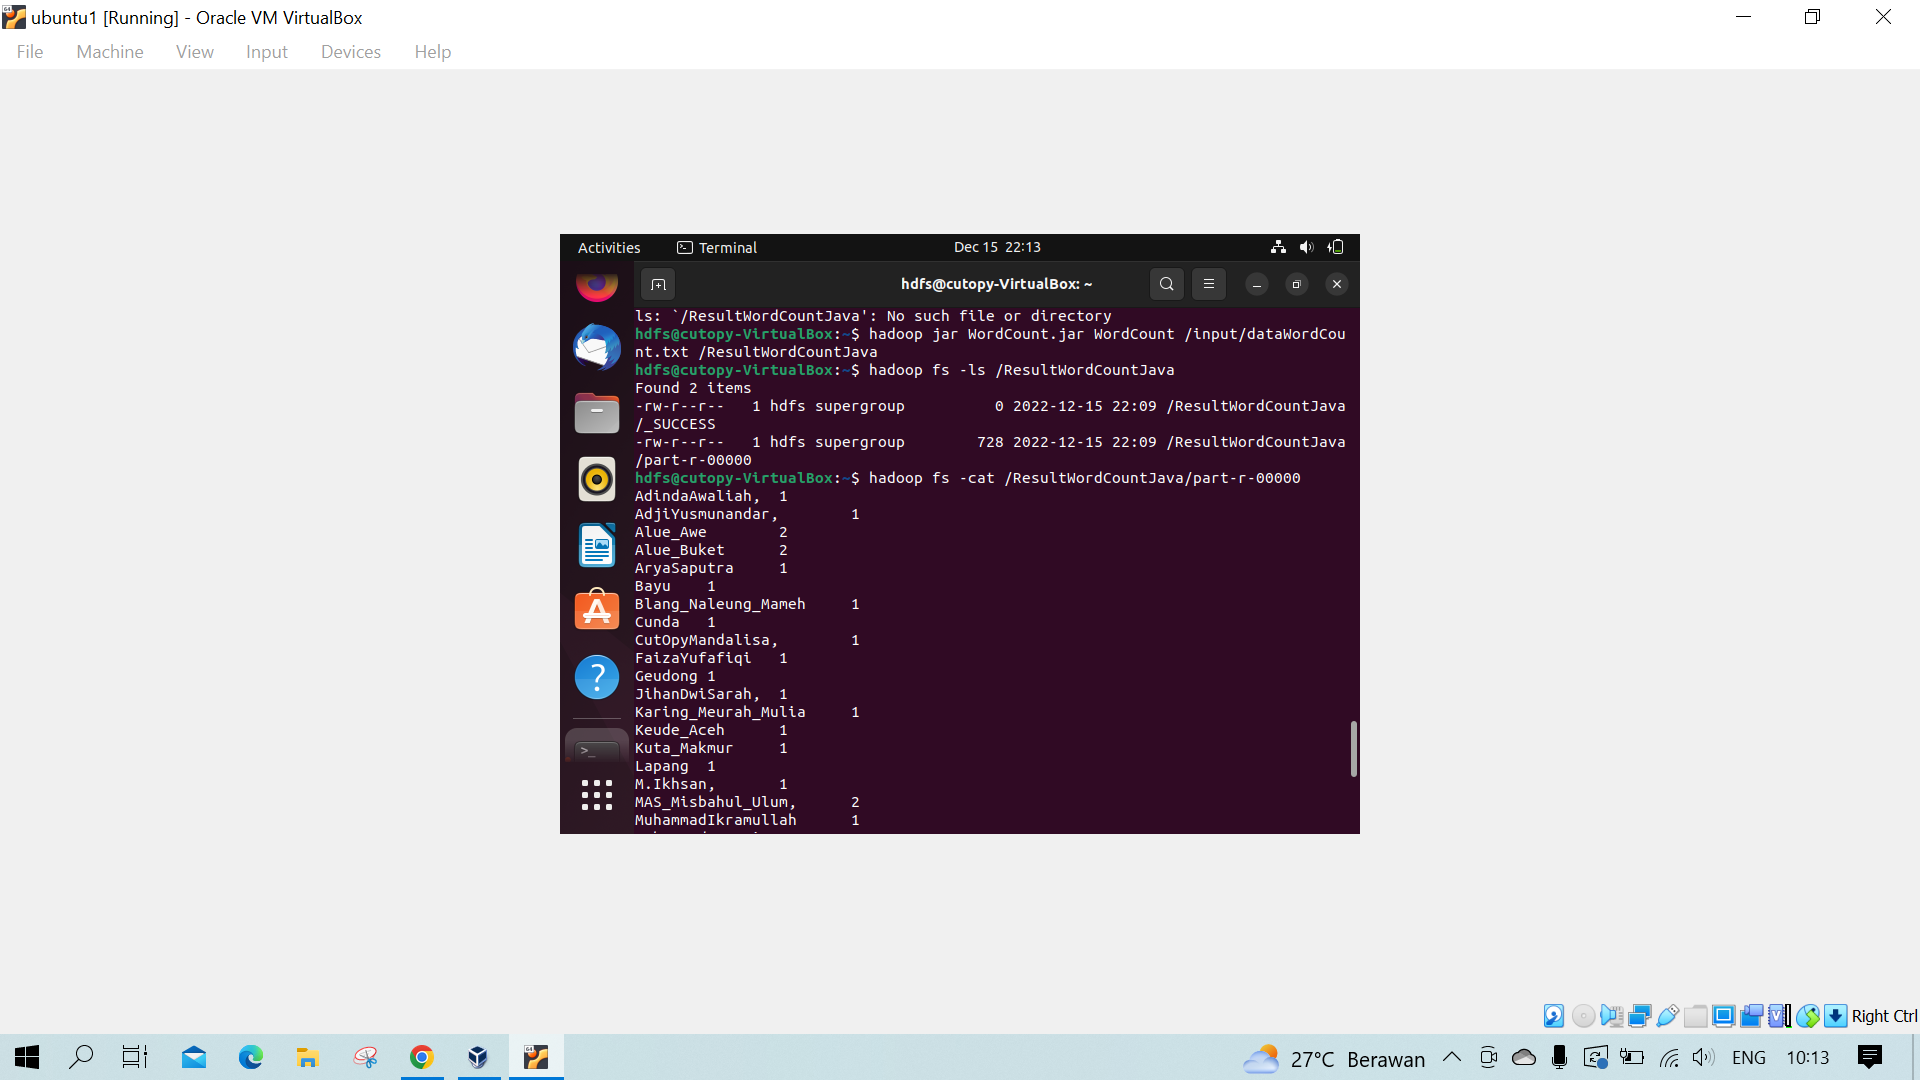
\includegraphics[width=\textwidth]{CutOpyMandalisa/04}
\caption{hasil wordCount dengan java}
\label{gam:perkuliahan-25-11}
\end{figure}

\item Kesimpulan\\
% berikan kesimpulan dari praktikum yang telah dikerjkan
Berhasil menjalankan program WordCount dengan java.
\end{enumerate}


\newday{\textbf{15 Desember 2022}}
\begin{enumerate}
\item Kendala dan Solusi
% jelaskan kendala dan penyebab yang dialami saat mengikuti praktikum serta solusi atau langkah-langkah yang telah dilakukan

\item Kesimpulan
% berikan kesimpulan dari praktikum yang telah dikerjkan
\end{enumerate}


\newday{\textbf{16 Desember 2022}}
\begin{enumerate}
\item Kendala dan Solusi
% jelaskan kendala dan penyebab yang dialami saat mengikuti praktikum serta solusi atau langkah-langkah yang telah dilakukan

\item Kesimpulan
% berikan kesimpulan dari praktikum yang telah dikerjkan
\end{enumerate}

\newday{\textbf{22 Desember 2022}}
\begin{enumerate}
\item Kendala dan Solusi
% jelaskan kendala dan penyebab yang dialami saat mengikuti praktikum serta solusi atau langkah-langkah yang telah dilakukan

\item Kesimpulan
% berikan kesimpulan dari praktikum yang telah dikerjkan
\end{enumerate}

\newday{\textbf{23 Desember 2022}}
\begin{enumerate}
\item Kendala dan Solusi
% jelaskan kendala dan penyebab yang dialami saat mengikuti praktikum serta solusi atau langkah-langkah yang telah dilakukan

\item Kesimpulan
% berikan kesimpulan dari praktikum yang telah dikerjkan
\end{enumerate}
\newthought{\textbf{Adinda Awaliah - 2020903430004 - TRKJ 3B}}

\newday{\textbf{22 September 2022}}
\begin{enumerate}
\item Kendala dan Solusi
% jelaskan kendala dan penyebab yang dialami saat mengikuti praktikum serta solusi atau langkah-langkah yang telah dilakukan

\item Kesimpulan
% berikan kesimpulan dari praktikum yang telah dikerjkan

\end{enumerate}


\newthought{\textbf{Jihan Dwi Sarah - 2020903430015 - TRKJ 3B}}


\newday{\textbf{1 - 2 Desember 2022} - Instalasi Hadoop}
\begin{enumerate}
\item Kendala dan Solusi
% jelaskan kendala dan penyebab yang dialami saat mengikuti praktikum serta solusi atau langkah-langkah yang telah dilakukan
\newline Pada pertemuan hari ini, kegiatan yang dilakukan adalah menginstall Apache Hadoop. Selama praktikum tidak mengalami kendala.

\item Kesimpulan \\
% berikan kesimpulan dari praktikum yang telah dikerjkan
Berhasil melakukan instalasi java tanpa ada bug atau error serta instalasi hadoop berikut ini gambar hasil verifikasi instalasi java version dan hadoop version 

\begin{figure}[!ht]
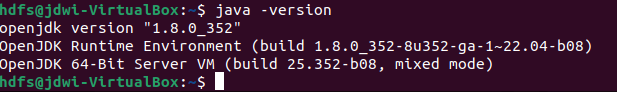
\includegraphics[width=\textwidth]{JihanDwiSarah/Java-version(Jihan)}
\caption{Verifikasi Hasil Instalasi Java}
\label{gam:Java-version(Jihan)}
\end{figure} 

\begin{figure}[!ht]
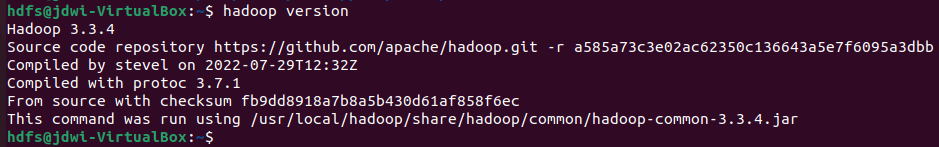
\includegraphics[width=\textwidth]{JihanDwiSarah/Hadoop-version(Jihan)}
\caption{Verifikasi Hasil Instalasi Hadoop}
\label{gam:Hadoop-version(Jihan)}
\end{figure}
\end{enumerate}


\newday{\textbf{8 - 9 Desember 2022} - Konfigurasi Hadoop}
\begin{enumerate}
\item Kendala dan Solusi \\
% jelaskan kendala dan penyebab yang dialami saat mengikuti praktikum serta solusi atau langkah-langkah yang telah dilakukan
Pada pertemuan hari ini, kegiatan yang dilakukan adalah mengkonfigurasi Apache Hadoop. Selama praktikum tidak mengalami kendala.

\item Kesimpulan \\
% berikan kesimpulan dari praktikum yang telah dikerjkan
Berhasil mengkonfigurasi beberapa file Hadoop sehingga memudahkan dalam memonitoring ekosistem Hadoop yang telah diinstall. Berikut ini gambar bukti keberhasilan praktikum. 

\begin{figure}[!ht]
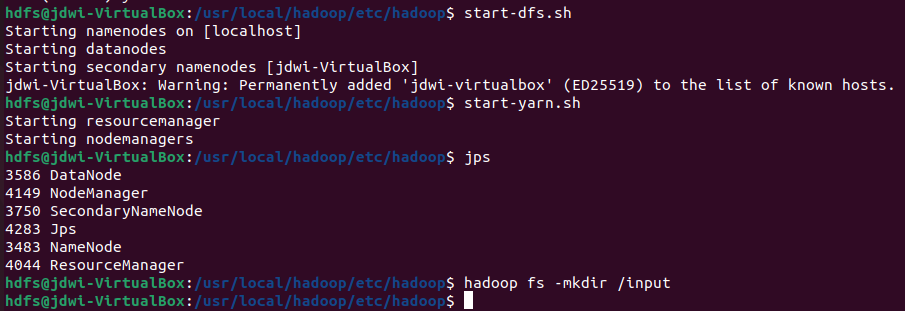
\includegraphics[width=\textwidth]{JihanDwiSarah/perintah-jps(jihan)}
\caption{Hasil perintah jps}
\label{gam:perintah-jps(jihan)}
\end{figure} 


\begin{figure}[!ht]
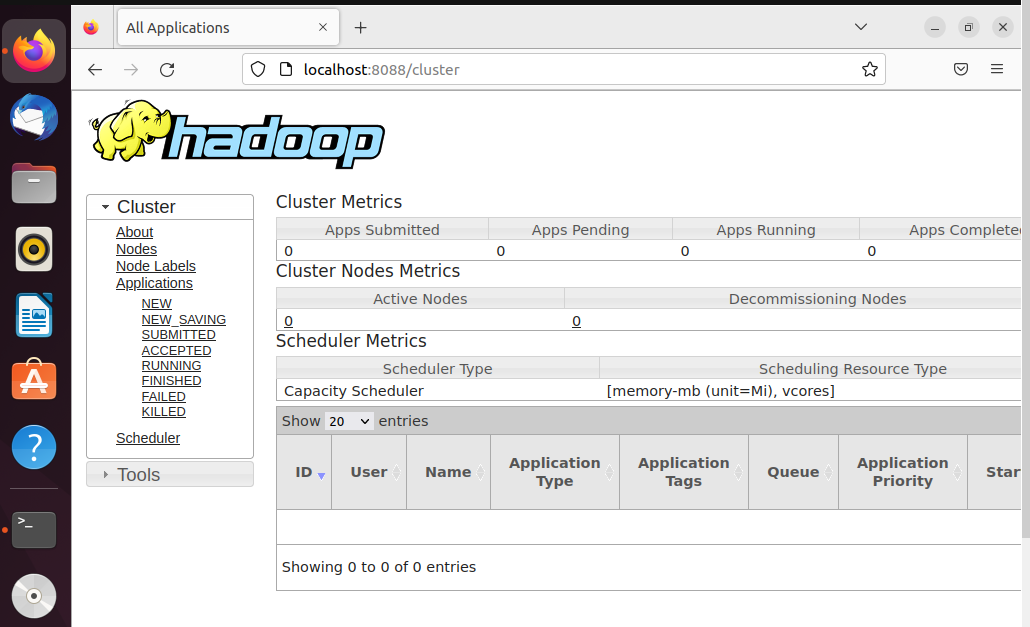
\includegraphics[width=\textwidth]{JihanDwiSarah/Akses-web-browser-8088(Jihan)}
\caption{Akses melalui web browser dengan alamat http://localhost:8088}
\label{gam:Akses-web-browser-8088(Jihan)}
\end{figure} 

\begin{figure}[!ht]
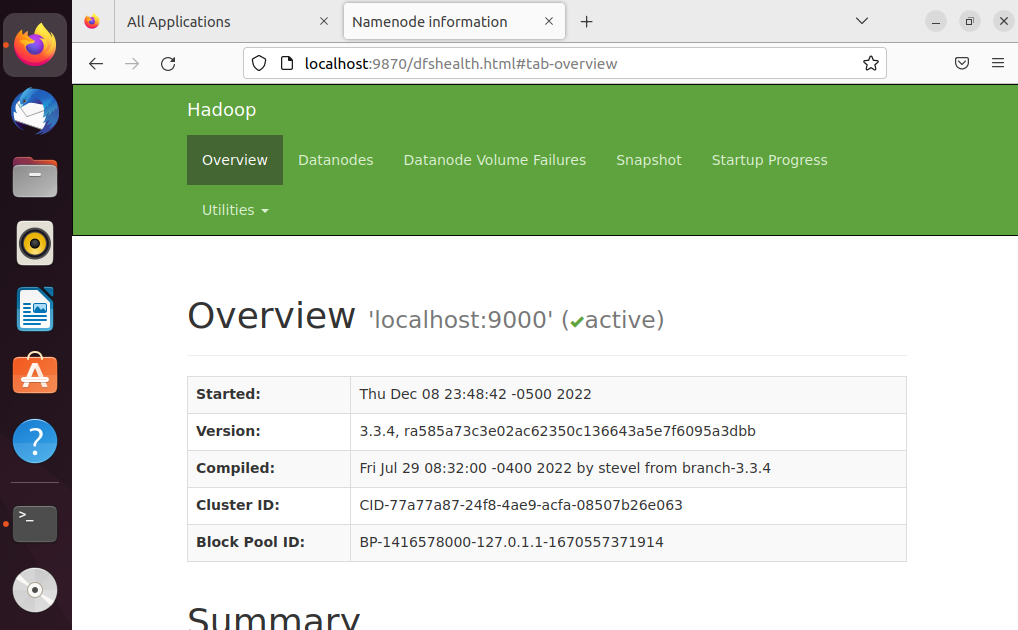
\includegraphics[width=\textwidth]{JihanDwiSarah/Akses-web-browser-9870(Jihan)}
\caption{Akses melalui web browser dengan alamat http://localhost:9870}
\label{gam:Akses-web-browser-9870(Jihan)}
\end{figure} 
\end{enumerate}

\newday{\textbf{15 Desember 2022} - WordCount Bawaan Hadoop}
\begin{enumerate}
\item Kendala dan Solusi \\
% jelaskan kendala dan penyebab yang dialami saat mengikuti praktikum serta solusi atau langkah-langkah yang telah dilakukan
Pada pertemuan hari ini, kegiatan yang dilakukan adalah mencoba program bawaan Hadoop untuk memahami bagaimana
proses dan cara kerja Hadoop dalam memproses data input hingga menghasilkan sebuah output. Selama praktikum tidak mengalami kendala.

\item Kesimpulan\\
% berikan kesimpulan dari praktikum yang telah dikerjkan
Berhasil mencoba program bawaan Hadoop yaitu program menghitung jumlah kata dalam data input yang diberikan.Berikut ini gambar bukti keberhasilan praktikum. 
\begin{figure}[!ht]
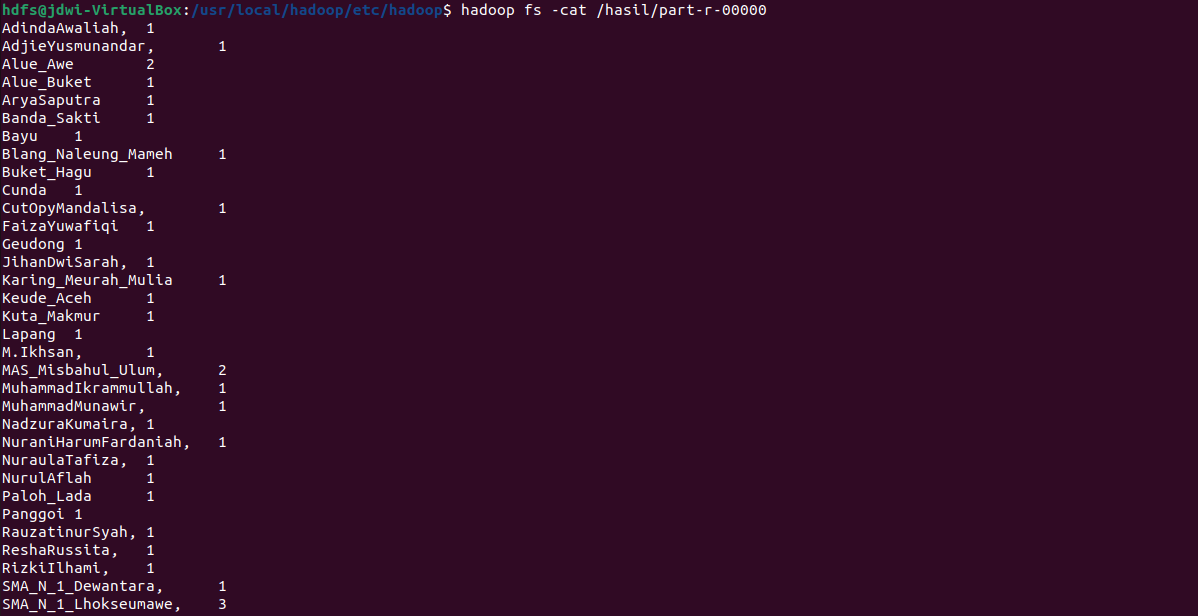
\includegraphics[width=\textwidth]{JihanDwiSarah/WordCount bawaan-Hadoop(jihan)}
\caption{Output Wordcount Bawaan Hadoop}
\label{gam:WordCount bawaan-Hadoop(jihan)}
\end{figure}
\end{enumerate}

\newday{\textbf{16 Desember 2022} - Program WordCount dengan Java}
\begin{enumerate}
\item Kendala dan Solusi \\
% jelaskan kendala dan penyebab yang dialami saat mengikuti praktikum serta solusi atau langkah-langkah yang telah dilakukan
Pada pertemuan hari ini, kegiatan yang dilakukan adalah mencoba program  wordcount dengan java. Selama praktikum mengalami kendala pada poin ke-6 berdasarkan urutan di modul. Program tidak mau dicompile karena kesalahan penulisan perintah.\\

solusinya adalah menggunakan perintah seperti berikut \\
\begin{figure}[!ht]

\includegraphics[width=\textwidth]{JihanDwiSarah/solusi-java-compile(jihan)}
\caption{Solusi Meng-Compile java}
\label{gam:solusi-java-compile(jihan)}
\end{figure}


\item Kesimpulan\\
% berikan kesimpulan dari praktikum yang telah dikerjkan
Dapat memberikan pemahaman mengenai proses membuat program wordcount java, menyiapkan data, meng-compile program hingga menjalankan program dan memperoleh hasilnya. Berikut hasil praktikum.

\begin{figure}[!ht]
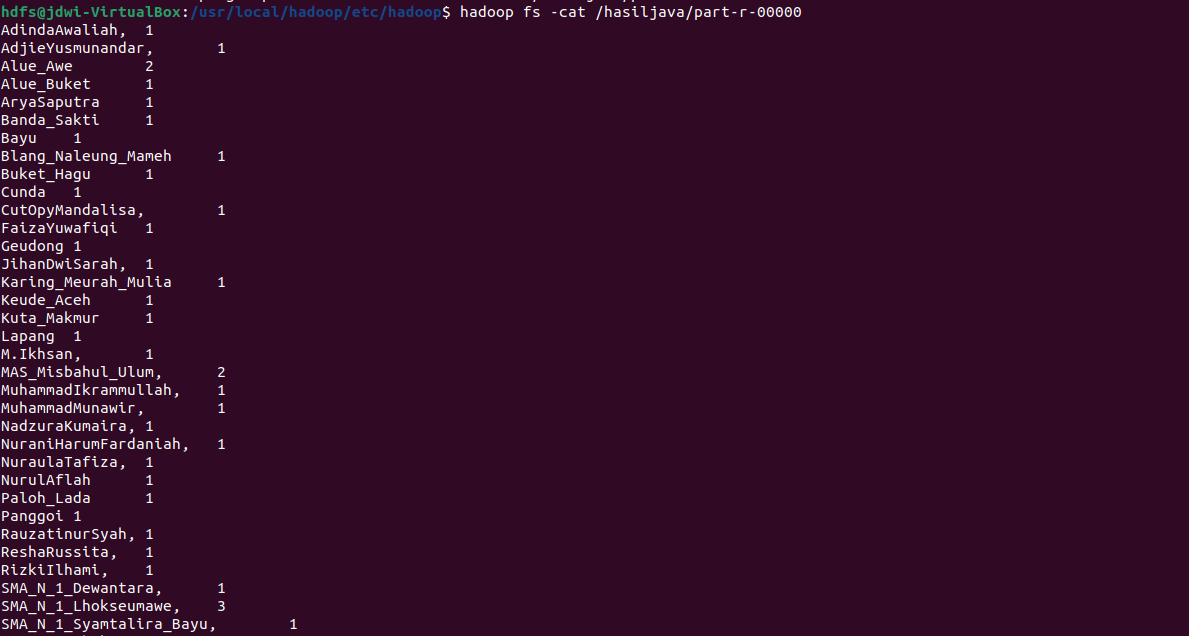
\includegraphics[width=\textwidth]{JihanDwiSarah/WordCount-Java(jihan)}
\caption{Output Wordcount java}
\label{gam:WordCount-Java(jihan)}
\end{figure}
\end{enumerate}

\newday{\textbf{17 Desember 2022} - Instalasi Apache Spark (PySpark)}
\begin{enumerate}
\item Kendala dan Solusi \\
% jelaskan kendala dan penyebab yang dialami saat mengikuti praktikum serta solusi atau langkah-langkah yang telah dilakukan
Terdapat kendala pada poin ke 3 karena kesalahan dari modulnya, perintah yang benar adalah sebagai berikut:\\
sudo mv spark-3.3.1-bin-hadoop3.\\
tidak perlu menambahkan '/usr/local/spark' lagi di akhir.


\item Kesimpulan\\
% berikan kesimpulan dari praktikum yang telah dikerjkan
Berhasil melakukan instalasi apache spark (PySpark), berikut hasil praktikum : \\

\begin{figure}[!ht]
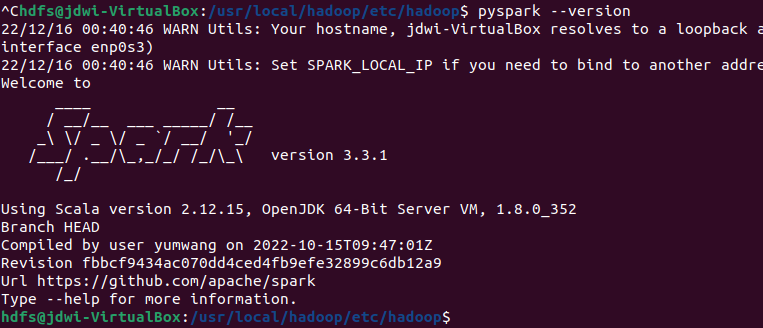
\includegraphics[width=\textwidth]{JihanDwiSarah/Instalasi-Spark(jihan)}
\caption{Hasil Instalasi Spark}
\label{gam:Instalasi-Spark(jihan)}
\end{figure}


\end{enumerate}


\newday{\textbf{22 Desember 2022} - Program WordCount dengan Python }
\begin{enumerate}
\item Kendala dan Solusi \\
% jelaskan kendala dan penyebab yang dialami saat mengikuti praktikum serta solusi atau langkah-langkah yang telah dilakukan


\item Kesimpulan\\
% berikan kesimpulan dari praktikum yang telah dikerjkan


\end{enumerate}

\newthought{\textbf{M.IKHSAN - 2020903430016 - TRKJ 3B}}

\newday{\textbf{01 Desember 2022}}
\begin{enumerate}
\item Kendala
% jelaskan kendala dan penyebab yang dialami saat mengikuti praktikum serta solusi atau langkah-langkah yang telah dilakukan
\newline 
1. saat mengintal apache hadoop, apache hadoopnya tidak selesai karena penyimpanan pada ubuntu penuh. jadi, saya menginstal ulang ubuntu untuk menambah penyimpanan
2. masih error saat menjalankan perintah start-dfs.sh 

solusi
\item Kesimpulan
% berikan kesimpulan dari praktikum yang telah dikerjkan

\end{enumerate}

\begin{figure}[!ht]
    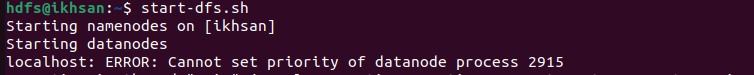
\includegraphics[width=\textwidth]{M.IKHSAN/Capture}
    \caption{error pada perintah start-hdfs.sh}
    \label{gam:Hasil}
\end{figure}

\newday{\textbf{02 Desember 2022}}
\begin{enumerate}
\item Kendala dan Solusi
% jelaskan kendala dan penyebab yang dialami saat mengikuti praktikum serta solusi atau langkah-langkah yang telah dilakukan

\item Kesimpulan
% berikan kesimpulan dari praktikum yang telah dikerjkan

\end{enumerate}

\newday{\textbf{08 Desember 2022}}
\begin{enumerate}
\item Kendala dan Solusi
% jelaskan kendala dan penyebab yang dialami saat mengikuti praktikum serta solusi atau langkah-langkah yang telah dilakukan

\item Kesimpulan
% berikan kesimpulan dari praktikum yang telah dikerjkan

\end{enumerate}


\newday{\textbf{09 Desember 2022}}
\begin{enumerate}
\item Kendala dan Solusi
% jelaskan kendala dan penyebab yang dialami saat mengikuti praktikum serta solusi atau langkah-langkah yang telah dilakukan


\item Kesimpulan
% berikan kesimpulan dari praktikum yang telah dikerjkan
\newline menginstal ulang ubuntu untuk menambah penyimpanan
\end{enumerate}

\newday{\textbf{15 Desember 2022}}
\begin{enumerate}
\item Kendala dan Solusi
% jelaskan kendala dan penyebab yang dialami saat mengikuti praktikum serta solusi atau langkah-langkah yang telah dilakukan

\item Kesimpulan
% berikan kesimpulan dari praktikum yang telah dikerjkan

\end{enumerate}

\newday{\textbf{16 Desember 2022}}
\begin{enumerate}
\item Kendala dan Solusi
% jelaskan kendala dan penyebab yang dialami saat mengikuti praktikum serta solusi atau langkah-langkah yang telah dilakukan

\item Kesimpulan
% berikan kesimpulan dari praktikum yang telah dikerjkan

\end{enumerate}

\newday{\textbf{22 Desember 2022}}
\begin{enumerate}
\item Kendala dan Solusi
% jelaskan kendala dan penyebab yang dialami saat mengikuti praktikum serta solusi atau langkah-langkah yang telah dilakukan

\item Kesimpulan
% berikan kesimpulan dari praktikum yang telah dikerjkan

\end{enumerate}

\newday{\textbf{23 Desember 2022}}
\begin{enumerate}
\item Kendala dan Solusi
% jelaskan kendala dan penyebab yang dialami saat mengikuti praktikum serta solusi atau langkah-langkah yang telah dilakukan

\item Kesimpulan
% berikan kesimpulan dari praktikum yang telah dikerjkan

\end{enumerate}
\newthought{\textbf{Adinda Awaliah - 2020903430004 - TRKJ 3B}}

\newday{\textbf{22 September 2022}}
\begin{enumerate}
\item Kendala dan Solusi
% jelaskan kendala dan penyebab yang dialami saat mengikuti praktikum serta solusi atau langkah-langkah yang telah dilakukan

\item Kesimpulan
% berikan kesimpulan dari praktikum yang telah dikerjkan

\end{enumerate}


\newthought{\textbf{Muhammad Munawir - 2020903430026 - TRKJ 3B}}

\newday{\textbf{1 September 2022}}
\begin{enumerate}
\item Kendala dan Solusi
% jelaskan kendala dan penyebab yang dialami saat mengikuti praktikum serta solusi atau langkah-langkah yang telah dilakukan

\item Kesimpulan
% berikan kesimpulan dari praktikum yang telah dikerjkan

\end{enumerate}

\newday{\textbf{2 Desember 2022}}
\begin{enumerate}
\item Kendala dan Solusi
% jelaskan kendala dan penyebab yang dialami saat mengikuti praktikum serta solusi atau langkah-langkah yang telah dilakukan

\item Kesimpulan
% berikan kesimpulan dari praktikum yang telah dikerjkan

\end{enumerate}

\newday{\textbf{8 Desember 2022}}
\begin{enumerate}
\item Kendala dan Solusi
% jelaskan kendala dan penyebab yang dialami saat mengikuti praktikum serta solusi atau langkah-langkah yang telah dilakukan

\item Kesimpulan
% berikan kesimpulan dari praktikum yang telah dikerjkan

\end{enumerate}

\newday{\textbf{9 Desember 2022}}
\begin{enumerate}
\item Kendala dan Solusi
% jelaskan kendala dan penyebab yang dialami saat mengikuti praktikum serta solusi atau langkah-langkah yang telah dilakukan

\item Kesimpulan
% berikan kesimpulan dari praktikum yang telah dikerjkan

\end{enumerate}
\newthought{\textbf{Adinda Awaliah - 2020903430004 - TRKJ 3B}}

\newday{\textbf{22 September 2022}}
\begin{enumerate}
\item Kendala dan Solusi
% jelaskan kendala dan penyebab yang dialami saat mengikuti praktikum serta solusi atau langkah-langkah yang telah dilakukan

\item Kesimpulan
% berikan kesimpulan dari praktikum yang telah dikerjkan

\end{enumerate}


\newthought{\textbf{Nurani Harum Fardaniah - 2020903430034 - TRKJ 3B}}

\newday{\textbf{1 - 2 Desember 2022} - Instalasi dan Konfigurasi Apache Hadoop}
\begin{enumerate}
\item Kendala dan Solusi \\
Kendala :\\
Saat melakukan penginstalan hadoop tidak ada kendala apapun. Namun pada saat melakukan konfigurasi hadoop terdapat kendala pada saat melakukan hdfs namenode -format. Perintah ini tidak mau dijalankan karena ada kesalahan dalam penulisan pada file core-site.xml
Saat melakukan perintah jps pun hanya menampilkan 1 saja.

Solusi :\\
Melakukan perubahan penulisan pada file core-site.xml, setelah itu perintah hdfs namenode -format dapat dijalankan dan saat melakukan perintah jps akhirnya muncul ada 5.

\item Kesimpulan \\
Praktikum penginstalan hadoop dan konfigurasi hadoop berhasil dijalankan sesuai perintah-perintah yang ada.

\begin{figure}[!ht]
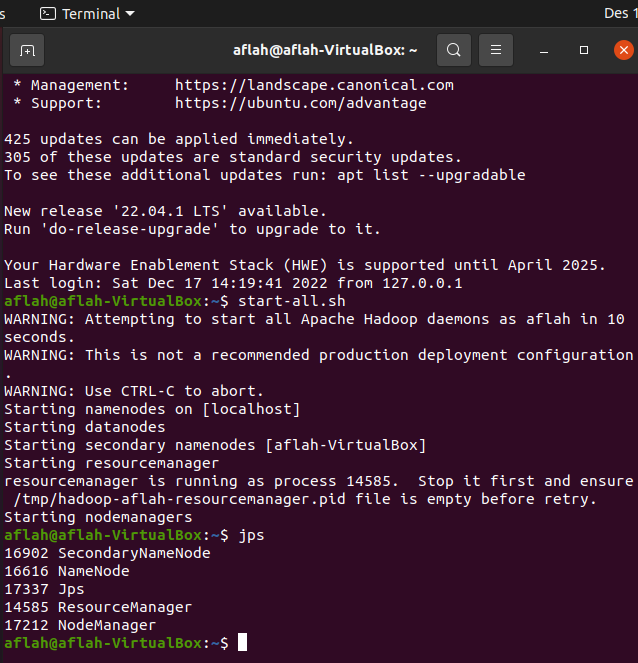
\includegraphics[width=\textwidth]{NuraniHarumFardaniah/jps}
\caption{hasil dari jps}
\label{gam:perkuliahan-25-11}
\end{figure}

\begin{figure}[!ht]
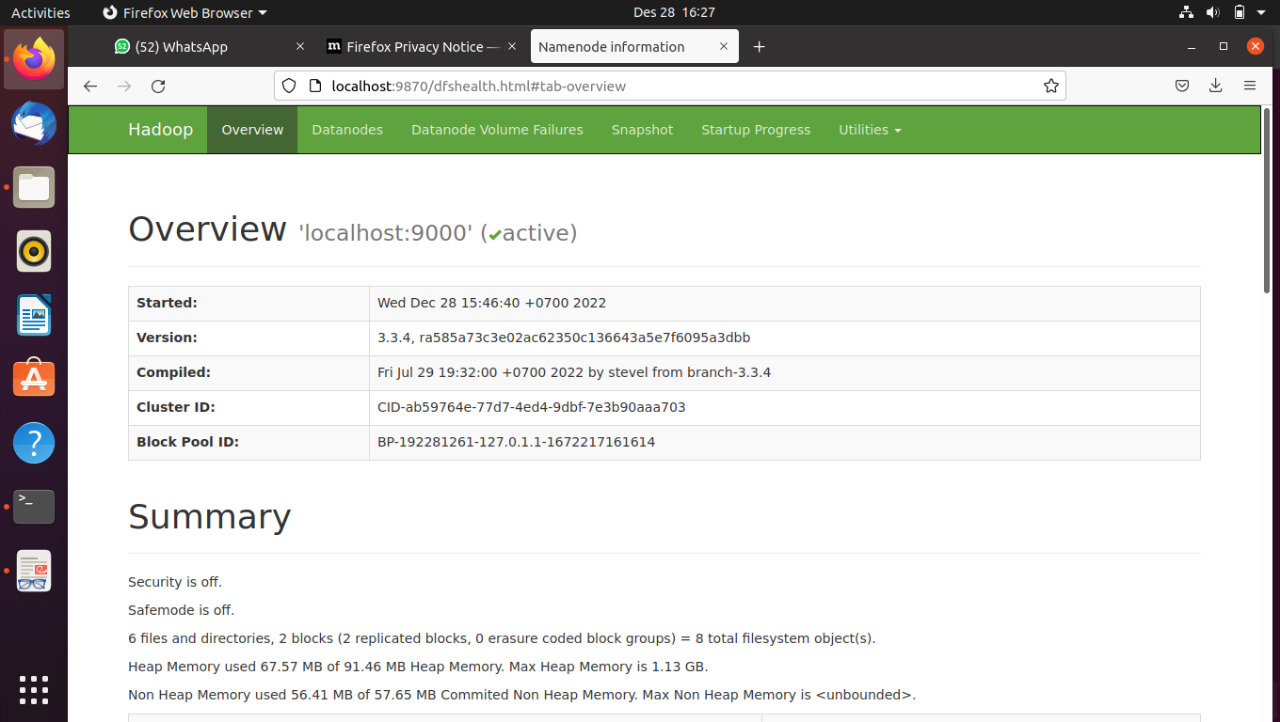
\includegraphics[width=\textwidth]{NuraniHarumFardaniah/localhost9870}
\caption{hasil dari localhost 9870}
\label{gam:perkuliahan-25-11}
\end{figure}

\newpage
\begin{figure}[!ht]
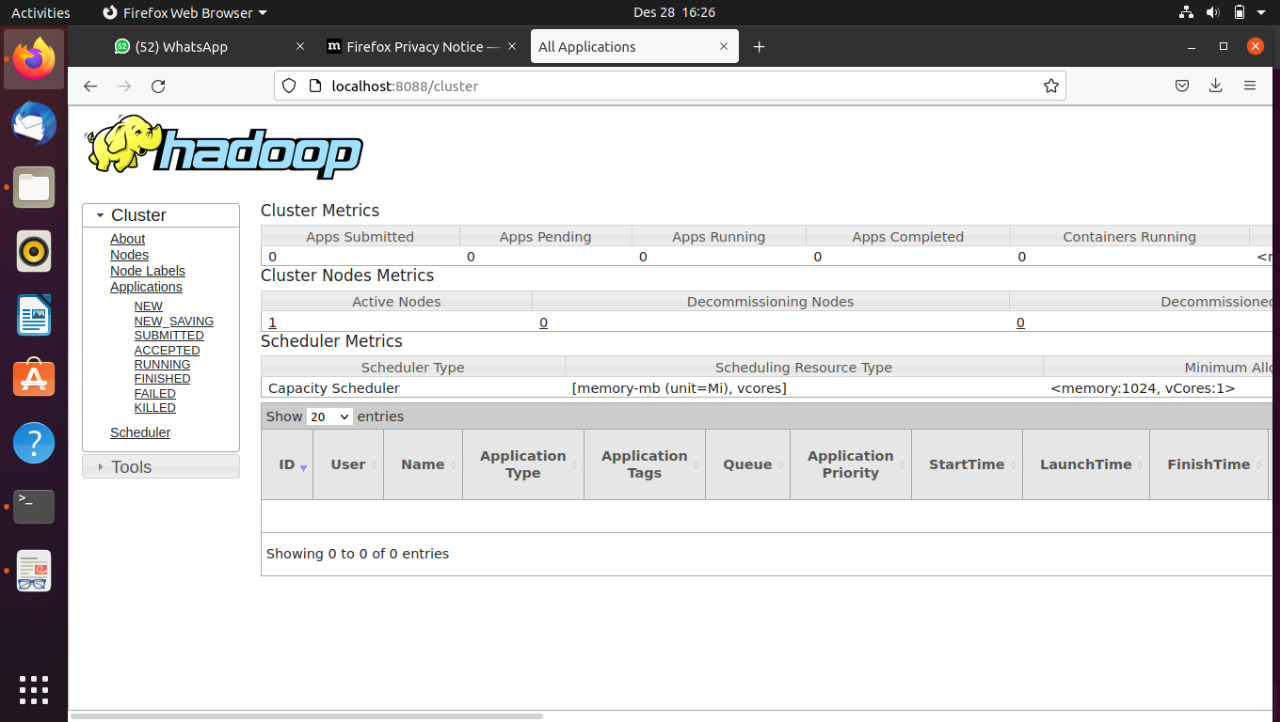
\includegraphics[width=\textwidth]{NuraniHarumFardaniah/localhost8088}
\caption{hasil dari localhost 8088}
\label{gam:perkuliahan-25-11}
\end{figure}

\end{enumerate}

\newday{\textbf{8 Desember 2022} - WordCount Bawaan Java}
\begin{enumerate}
\item Kendala dan Solusi
\newline Tidak ada kendala apapun saat melakukan program WordCount bawaan Hadoop

\item Kesimpulan
\newline Praktikum berhasil dilakukan sesuai dengan perintah-perintah yang ada. WordCount sendiri merupakan program untuk menghitung jumlah kata yang ada pada data.


\begin{figure}[!ht]
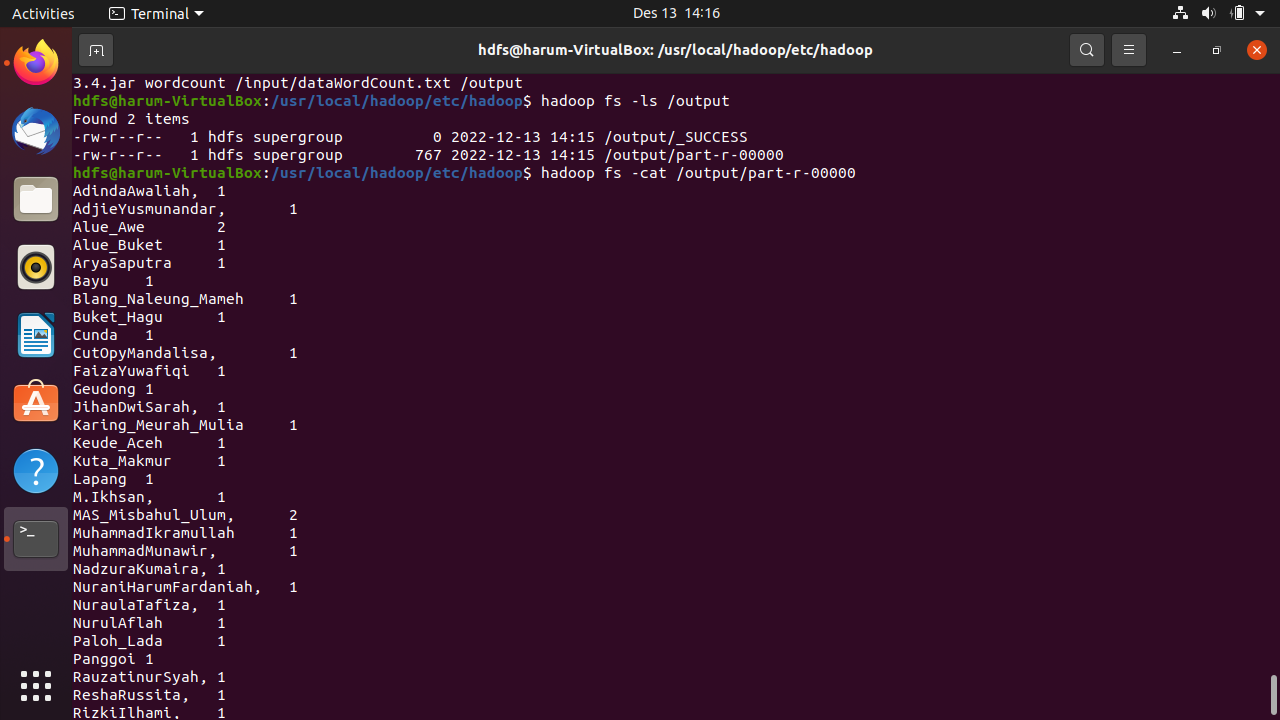
\includegraphics[width=\textwidth]{NuraniHarumFardaniah/6-7a}
\caption{Hasil dari langkah 6 dan 7}
\label{gam:perkuliahan-25-11}
\end{figure}
\newpage
\begin{figure}[!ht]
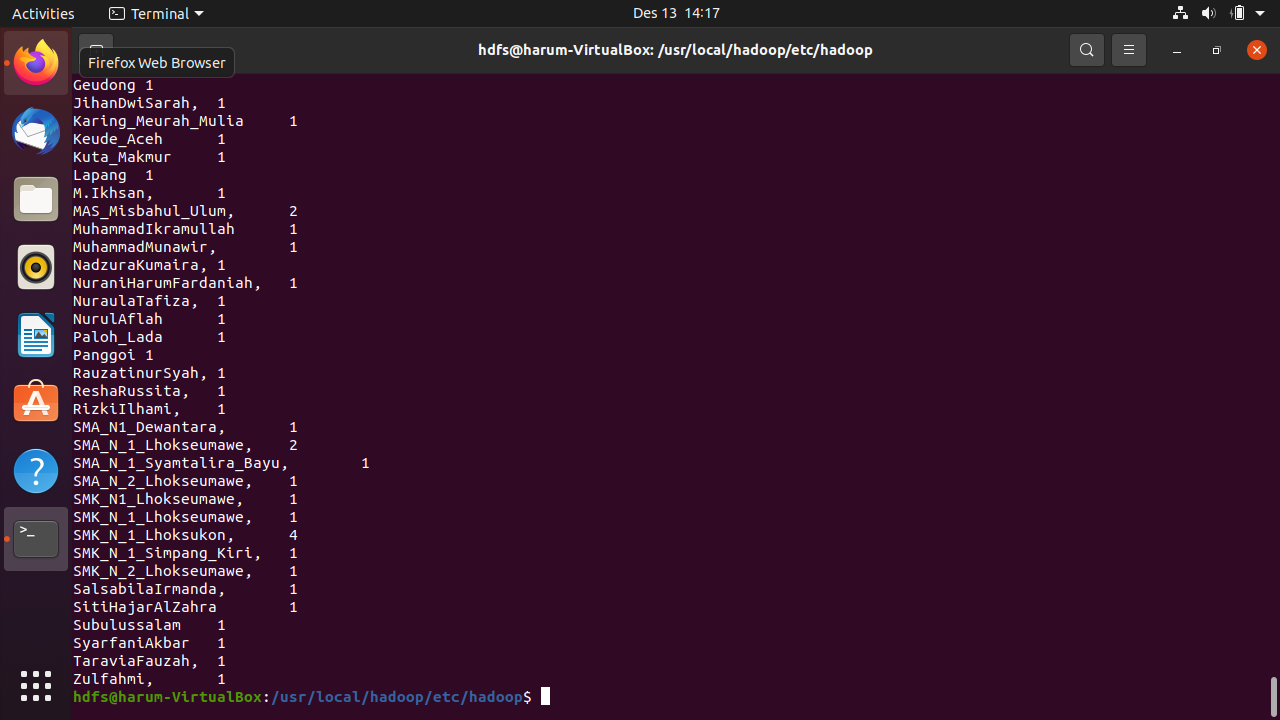
\includegraphics[width=\textwidth]{NuraniHarumFardaniah/7b}
\caption{Hasil dari langkah 7}
\label{gam:perkuliahan-25-11}
\end{figure}

\end{enumerate}

\newday{\textbf{9 Desember 2022} - WordCount dengan Java}
\begin{enumerate}
\item Kendala dan Solusi
\newline Kendala :\\
Saat melakukan praktikum program WordCount dengan Java terdapat kendala pada saat melakukan compile file WordCount. Perintah ini tidak mau dijalankan karena ada kesalahan dalam penulisan pada file WordCount.java

Solusi :\\
Melakukan perubahan penulisan pada file WordCount.java, setelah itu perintah untuk melakukan compile pada file WordCount.java dapat dijalankan.

\item Kesimpulan
\newline Praktikum berhasil dilakukan sesuai dengan perintah-perintah yang ada. Data pada WordCount dapat ditampilkan sesuai dengan yang telah dibuat.


\begin{figure}[!ht]
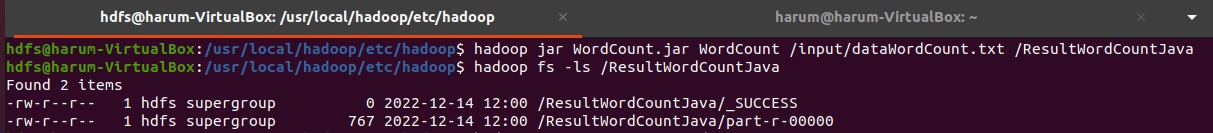
\includegraphics[width=\textwidth]{NuraniHarumFardaniah/9}
\caption{Hasil Perhitungan dengan WordCount Hadoop}
\label{gam:perkuliahan-25-11}
\end{figure}

\begin{figure}[!ht]
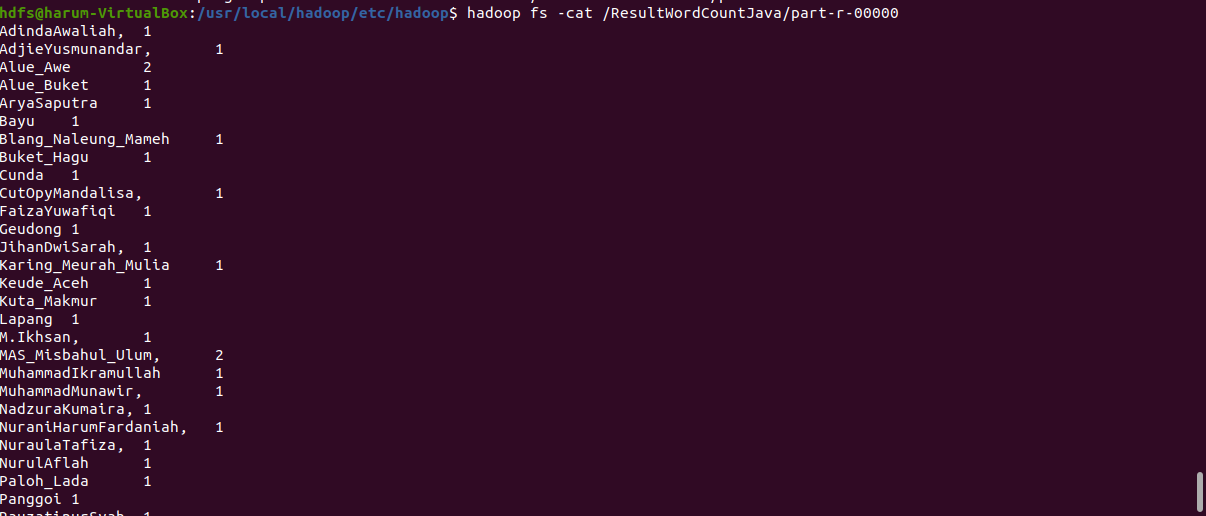
\includegraphics[width=\textwidth]{NuraniHarumFardaniah/10a}
\caption{Hasil Perhitungan dengan WordCount Hadoop}
\label{gam:perkuliahan-25-11}
\end{figure}
\newpage
\begin{figure}[!ht]
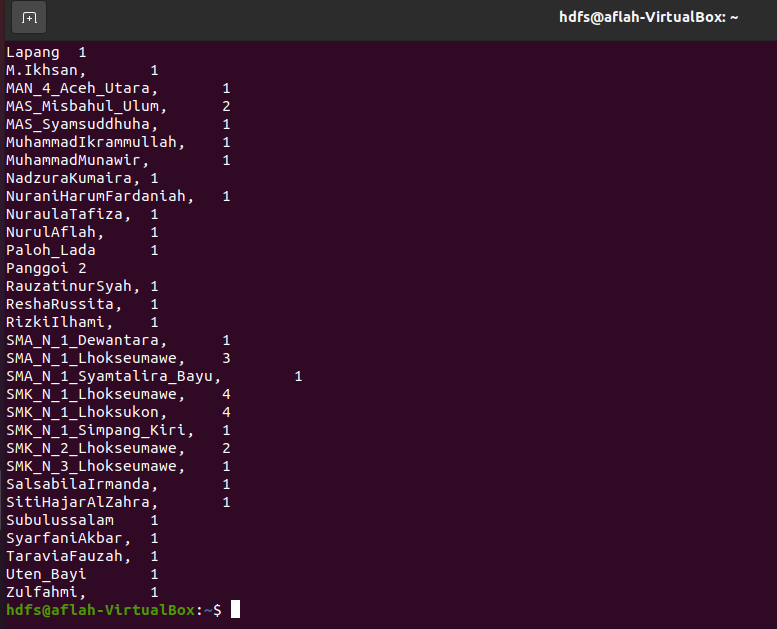
\includegraphics[width=\textwidth]{NuraniHarumFardaniah/10b}
\caption{Hasil Perhitungan dengan WordCount Hadoop}
\label{gam:perkuliahan-25-11}
\end{figure}

\end{enumerate}

\newday{\textbf{15 Desember 2022}} 
\begin{enumerate}
\item Kendala dan Solusi

\item Kesimpulan

\end{enumerate}
\newthought{\textbf{Adinda Awaliah - 2020903430004 - TRKJ 3B}}

\newday{\textbf{22 September 2022}}
\begin{enumerate}
\item Kendala dan Solusi
% jelaskan kendala dan penyebab yang dialami saat mengikuti praktikum serta solusi atau langkah-langkah yang telah dilakukan

\item Kesimpulan
% berikan kesimpulan dari praktikum yang telah dikerjkan

\end{enumerate}


\newthought{\textbf{Adinda Awaliah - 2020903430004 - TRKJ 3B}}

\newday{\textbf{22 September 2022}}
\begin{enumerate}
\item Kendala dan Solusi
% jelaskan kendala dan penyebab yang dialami saat mengikuti praktikum serta solusi atau langkah-langkah yang telah dilakukan

\item Kesimpulan
% berikan kesimpulan dari praktikum yang telah dikerjkan

\end{enumerate}


\newthought{\textbf{Rauzatinur Syah - 2020903430039 - TRKJ 3B}}


\newday{\textbf{1 - 2 Desember 2022} - Instalasi dan Konfigurasi Hadoop}
\begin{enumerate}
\item Kendala dan Solusi\\
% jelaskan kendala dan penyebab yang dialami saat mengikuti praktikum serta solusi atau langkah-langkah yang telah dilakukan
\begin{enumerate}
\item Kendala
\begin{itemize}
\item terdapat kendala pada instalasi hadoop pada pengecekanan versi hadoop yang berfungsi untuk menverifikasi instalasi hadoop
\item terdapat kendala saat menjalanakn format HDFS dan hadoop service
\end{itemize}
\item Solusi \\
\begin{itemize}
\item melakukan pengecekan pada file hadoop-env.sh
\item melakuka  pengecekan pada file core-site.xml, hdfs-site.xml, mapred-site.xml, yarn-site.xml
\end{itemize}
\end{enumerate}

\item Kesimpulan\\
% berikan kesimpulan dari praktikum yang telah dikerjkan
adapun kesimpulan yang diperoleh yaitu instalasi dan konfigurasi hadoop berhasil 
\end{enumerate}

\begin{figure}[!ht]
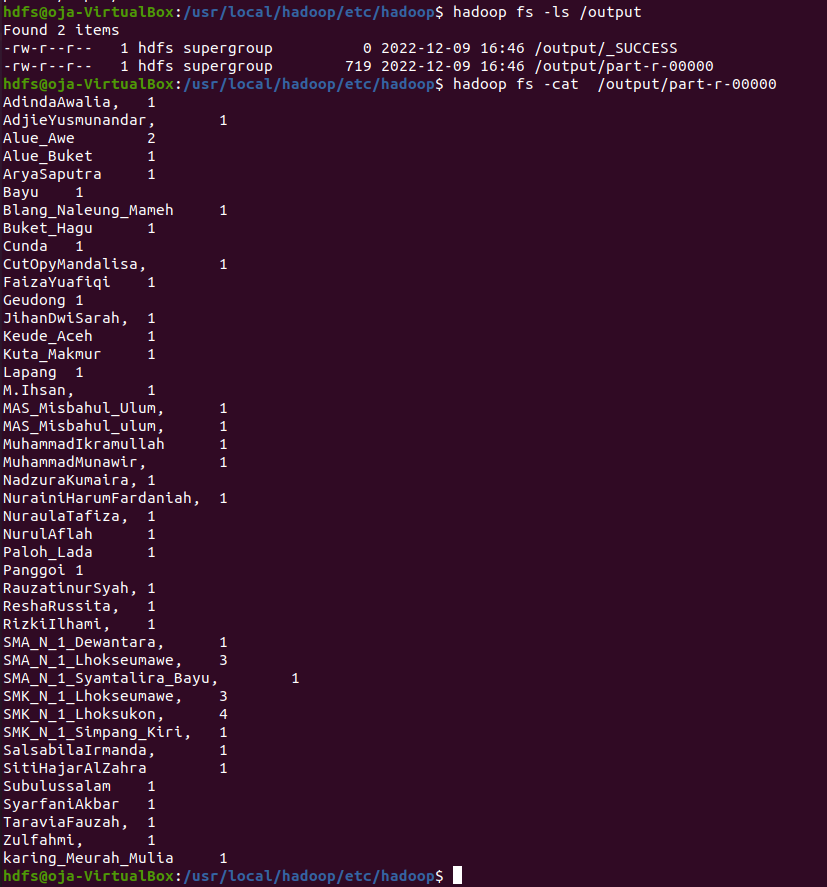
\includegraphics[width=\textwidth]{RauzatinurSyah/dataHadoop}
\caption{hasil program WordCount hadoop}
\label{gam:Hasil}
\end{figure}

\newday{\textbf{8 Desember 2022} - WordCount bawaan Hadoop}
\begin{enumerate}
\item Kendala dan Solusi\\
% jelaskan kendala dan penyebab yang dialami saat mengikuti praktikum serta solusi atau langkah-langkah yang telah dilakukan
pada pratikum Program WordCount bawaan hadoop tidak ada kendala pada praktikum yang dilakukan
\item Kesimpulan\\
% berikan kesimpulan dari praktikum yang telah dikerjkan
berhasil menjalanakan program wordCount bawan hadoop
\end{enumerate}


\begin{figure}[!ht]
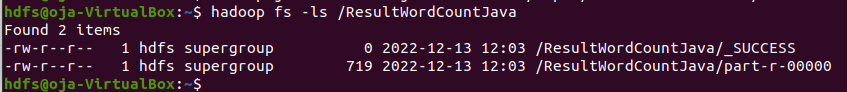
\includegraphics[width=\textwidth]{RauzatinurSyah/datahadoopjava no 9}
\caption{hasil program WordCount java no.9}
\label{gam:hasil program}
\end{figure}

\begin{figure}[!ht]
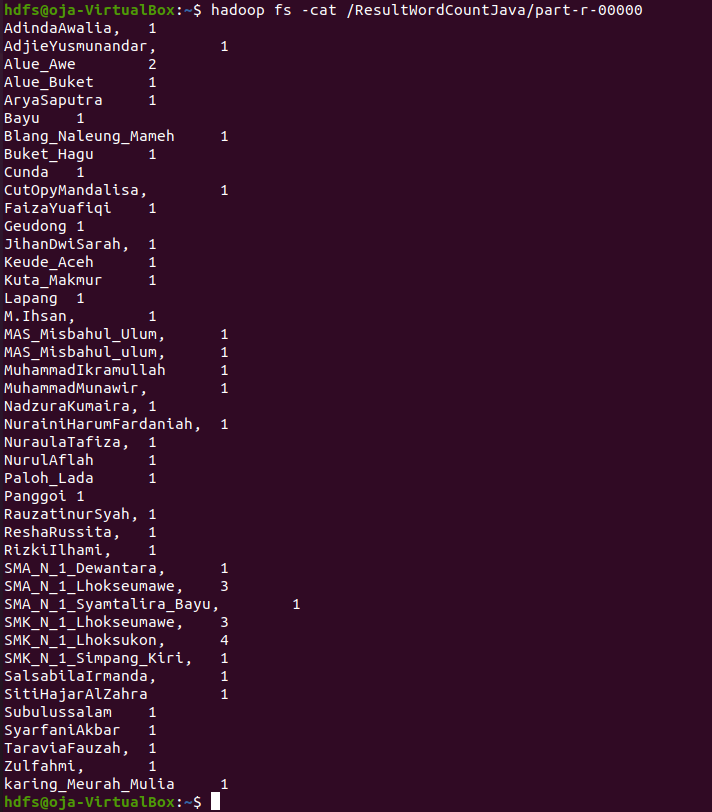
\includegraphics[width=\textwidth]{RauzatinurSyah/datahadoopjava no 10}
\caption{hasil program WordCount java no.10}
\label{gam:hasil program}
\end{figure}

\newday{\textbf{9 Desember 2022} - WordCount dengan Java}
\begin{enumerate}
\item Kendala dan Solusi \\
% jelaskan kendala dan penyebab yang dialami saat mengikuti praktikum serta solusi atau langkah-langkah yang telah dilakukan
pada praktikum WordCount dengan java
\begin{enumerate}
\item kendala: \\
terdapat kendala pada perintah menjalankan program dengan perintah"hadoop jar WordCount.jar WordCount /input/data/WordCount.txt /ResultWourdCountJava"
\item solusi: \\
menjalankan hadoop service dengan perintah "start-all.sh" dikarnakan terdapat kesalahan yang dilakukan yaitu tidak menjalankan hadoop service
\end{enumerate}
\item Kesimpulan\\
% berikan kesimpulan dari praktikum yang telah dikerjkan
adapun kesimpulan yang diperoleh yaitu berhasil menjalankan programa tersebut 
\end{enumerate}

\newday{\textbf{15 Desember 2022}}
\begin{enumerate}
\item Kendala dan Solusi\\
% jelaskan kendala dan penyebab yang dialami saat mengikuti praktikum serta solusi atau langkah-langkah yang telah dilakukan
pada instalasi apache spark tidak ada kendala yang dialami 
\item Kesimpulan\\
% berikan kesimpulan dari praktikum yang telah dikerjkan
apache spark berhasil dijalankan

\end{enumerate}

\begin{figure}[!ht]
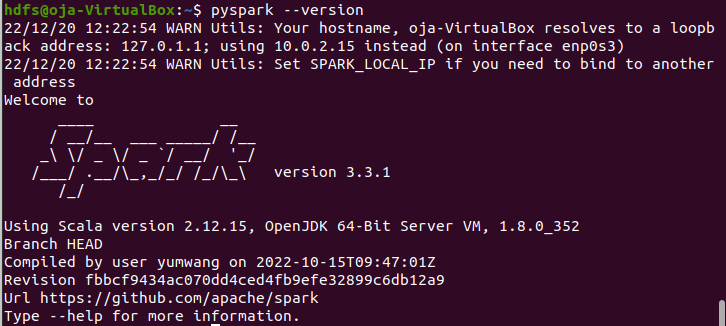
\includegraphics[width=\textwidth]{RauzatinurSyah/install spark}
\caption{hasil instalasi apache spark }
\label{gam:hasil instalasi spark}
\end{figure}


\newday{\textbf{16 Desember 2022}}
\begin{enumerate}
\item Kendala dan Solusi
% jelaskan kendala dan penyebab yang dialami saat mengikuti praktikum serta solusi atau langkah-langkah yang telah dilakukan

\item Kesimpulan
% berikan kesimpulan dari praktikum yang telah dikerjkan

\end{enumerate}

\newthought{\textbf{Resha Russita - 2020903430040 - TRKJ 3B}}

\newday{\textbf{22 September 2022}}
\begin{enumerate}
\item Kendala dan Solusi
Pada Instalasi Apache Hadoop, saya sebagai praktikan mengalami kendala saat mengekstrak file Apache Hadoop. Solusi yang saya gunakan adalah membuat kembali os ubuntu dengan ukuran ruang yang lebih besar dari sebelumnya sehingga file yang diekstrak berhasil. 
Kendala lain yang terjadi adalah hanya kurang teliti saat melakukan konfigurasi pada Apache Hadoop.

\begin{figure}[!ht]
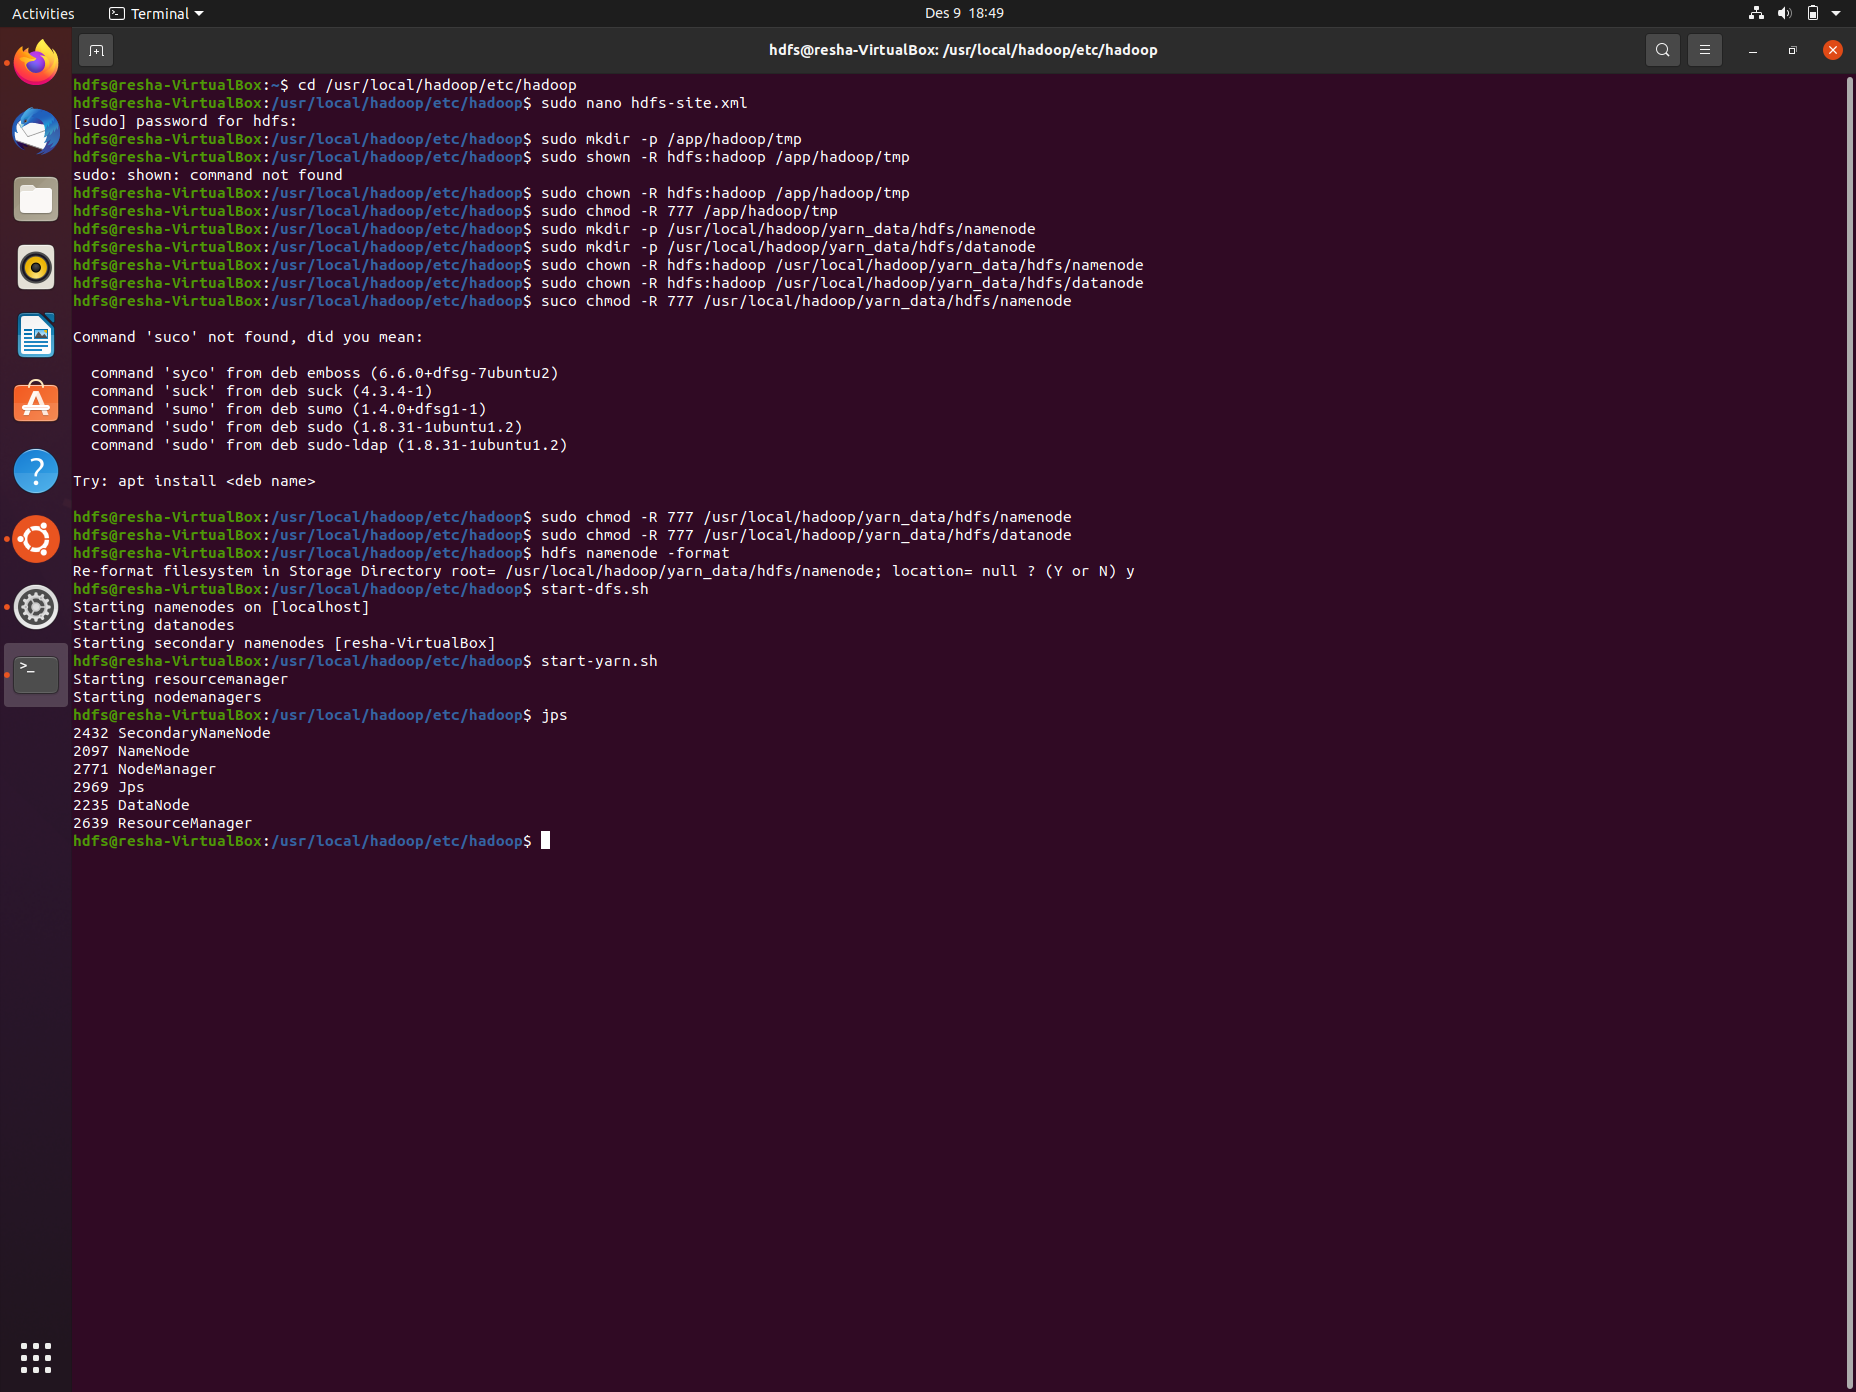
\includegraphics[width=\textwidth]{jpshadoopservice-resha}
\caption{cek services hadoop dengan jps}
\label{gam:perkuliahan-22-09}
\end{figure}

\begin{figure}[!ht]
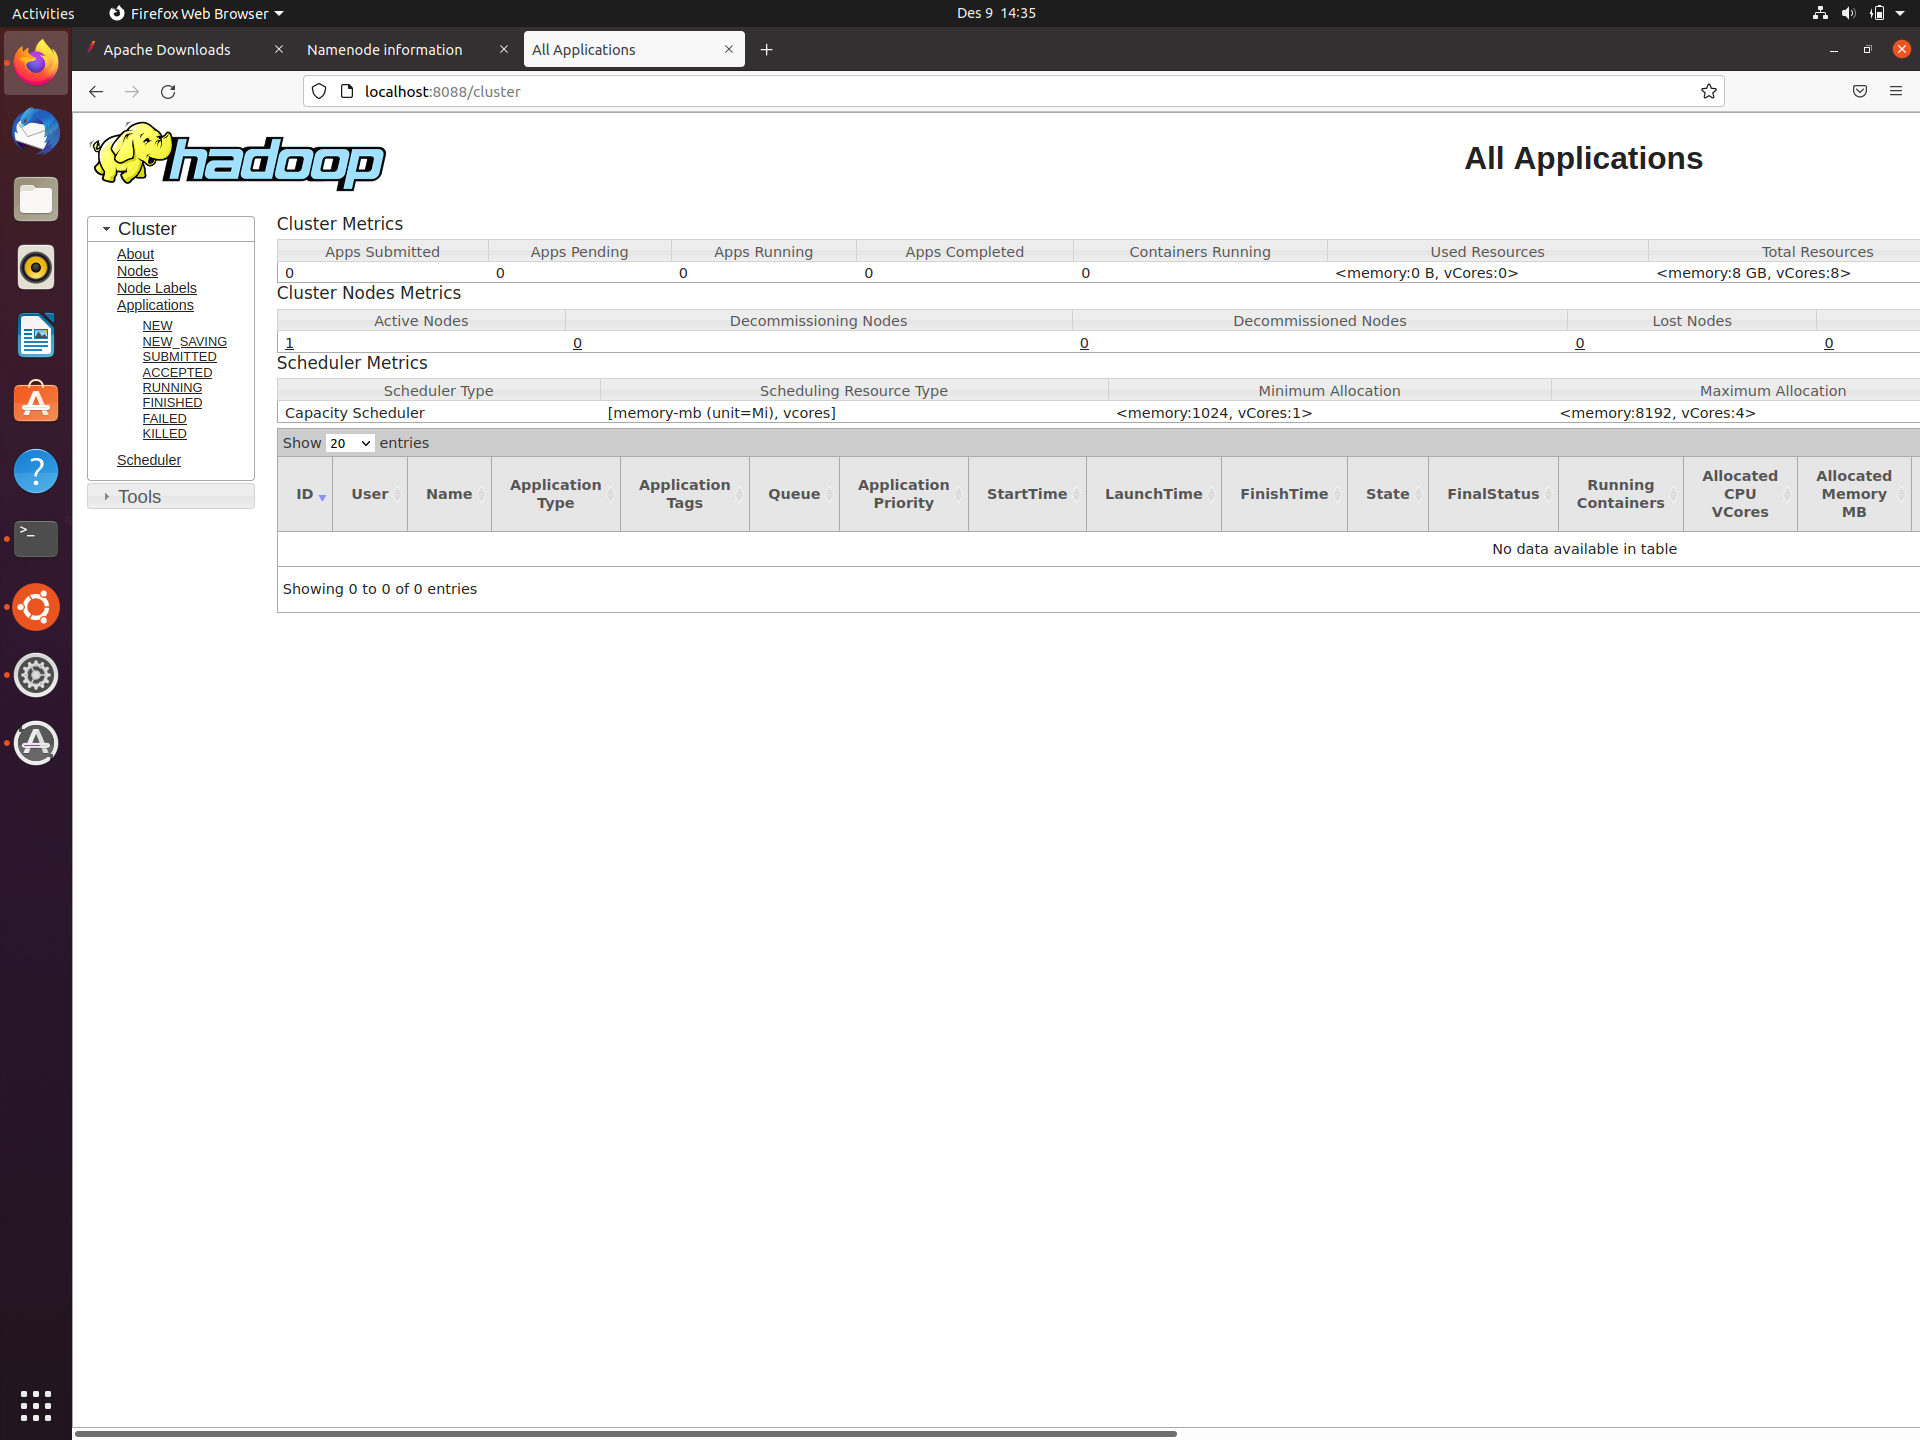
\includegraphics[width=\textwidth]{localhost8088-resha}
\caption{local host 8088 akses}
\label{gam:perkuliahan-22-09}
\end{figure}

\begin{figure}[!ht]
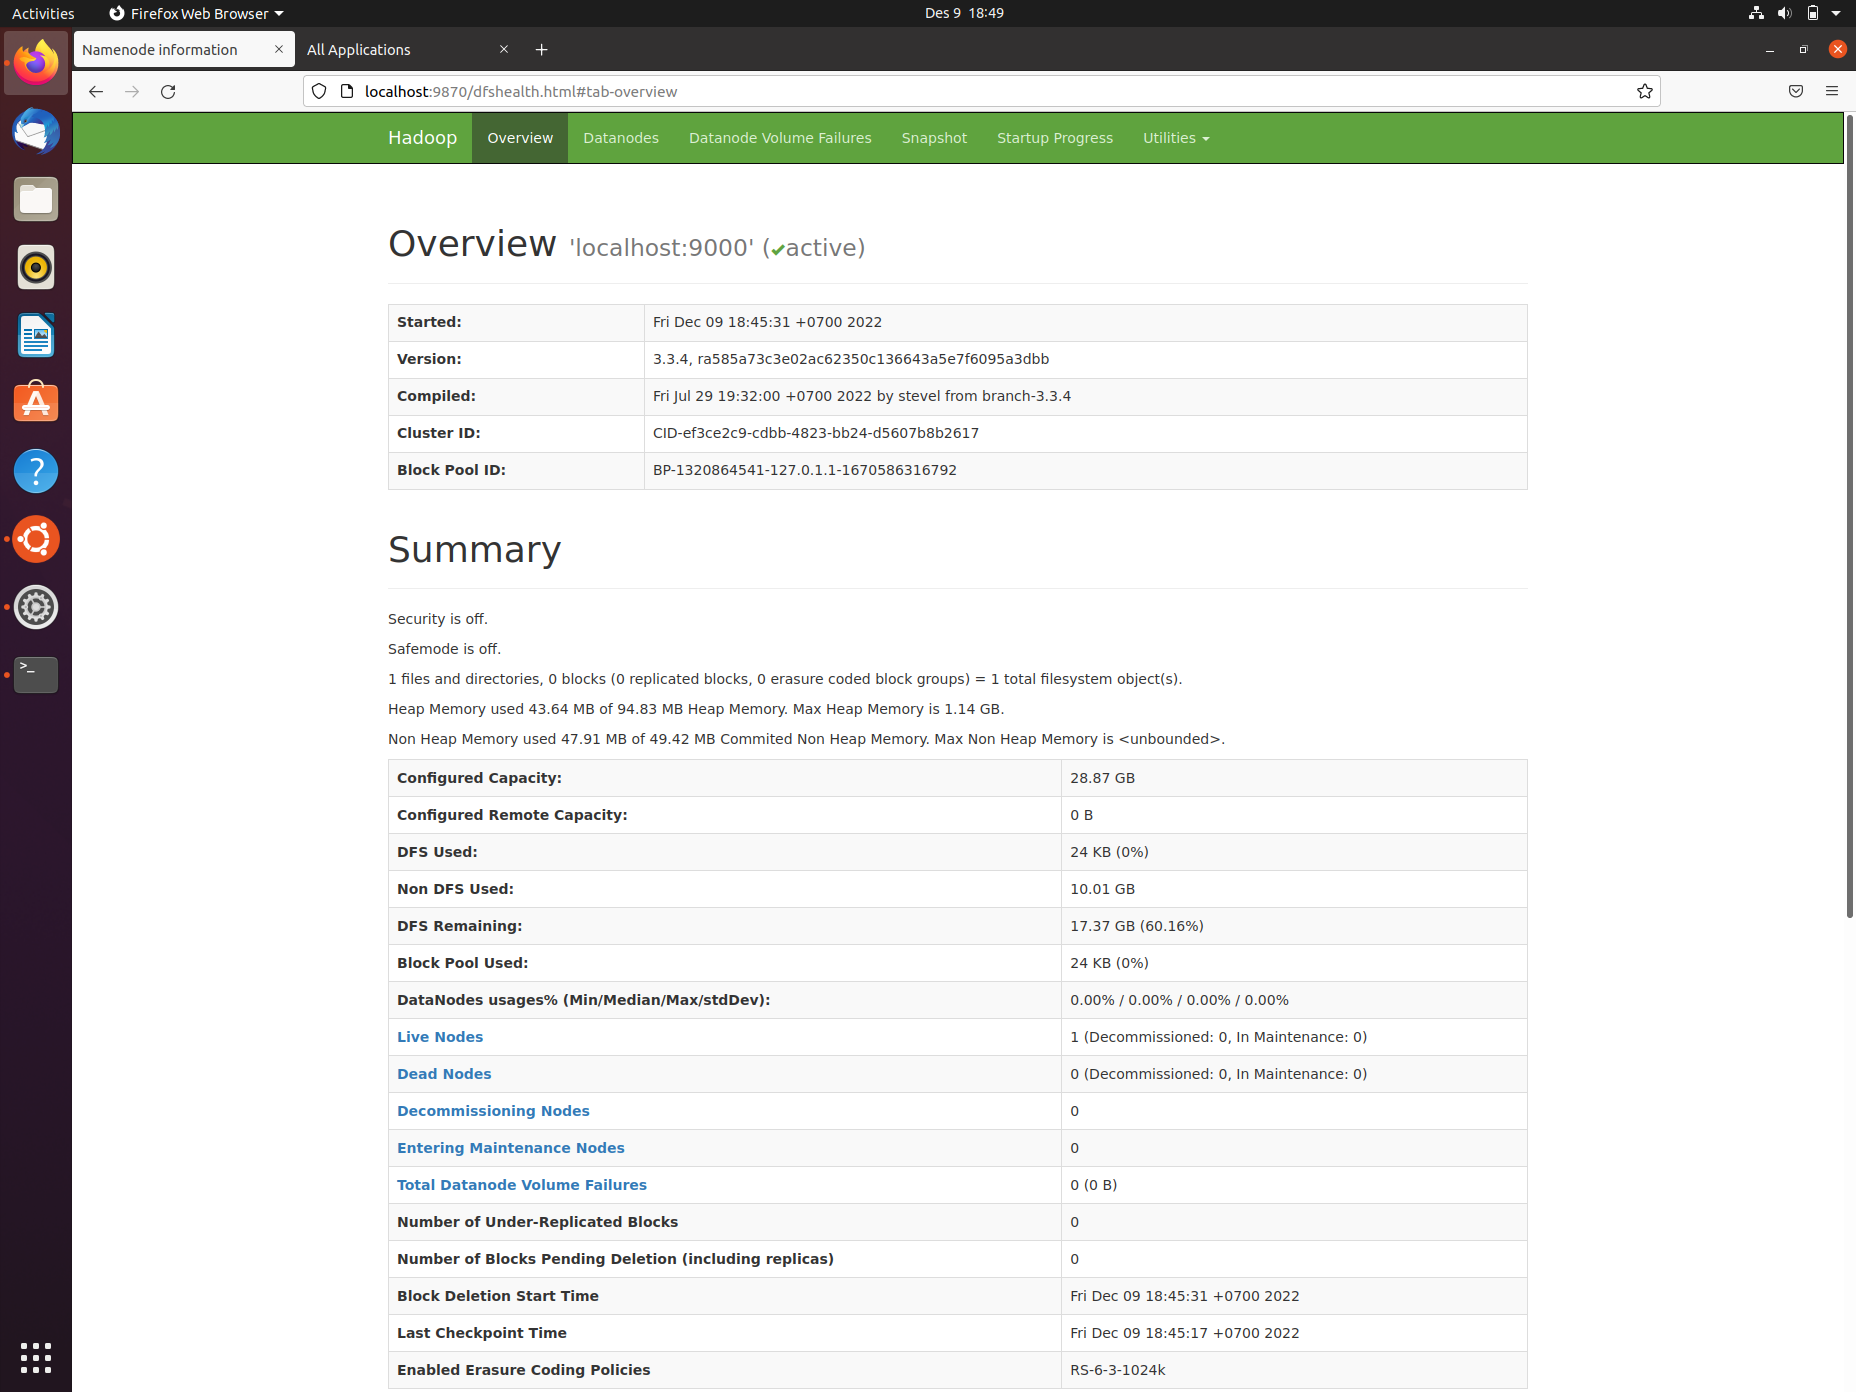
\includegraphics[width=\textwidth]{localhost9870-resha}
\caption{local host 9870 akses}
\label{gam:perkuliahan-22-09}
\end{figure}

\item Kesimpulan
Pada Instalasi Apache Hadoop membutuhkan ruang yang cukup besar untuk mengekstrak file Apache Hadoop. Penginstalaan Apache Hadoop harus dilakukan sesuai step, begitu juga pada saat konfigurasi. Konfigurasi ini bertujuan untuk memudahkan user dalam memonitoring ekosistem di dalam Hadoop. Saat mengkonfigurasi terdapat perintah untuk membuat format HDFS yang berfungsi menyimpan suatu data dengan cara membaginya menjadi potong-potongan data yang disebut blok berukuran 64 MB dan kemudian disimpan pada node-node yang tersebar dalam kluster. Node-node yang ada adalah name node dan data node. Sehingga saat mengecek Hadoop service dengan perintah jps, kedua node tersebut harus tersedia sebagai pendukung saat dilakukan akses web browser dengan local host 9870 dan 8088 berhasil.

\end{enumerate}

\newday{\textbf{24 November 2022}}
\begin{enumerate}
\item Kendala dan Solusi
Pada proses instalasi git dan konfigurasi git dengan github, saya sebagai praktikan tidak mengalami kendala sama sekali.

\item Kesimpulan
Pada instalasi git dan konfigurasi git dengan github bertujuan untuk menjalankan perintah-perintah git melalui penyimpan local dan menyimpan hasil pekerjaan pada github. Penyimpanan pekerjaan dapat dilakukan dengan mudah pada github dengan hanya melakukan git push.

\end{enumerate}

\newday{\textbf{01 Desember 2022}}
\begin{enumerate}
\item Kendala dan Solusi
Pada program WordCount bawaan Hadoop, tidak ada kendala yang saya alami.

\begin{figure}[!ht]
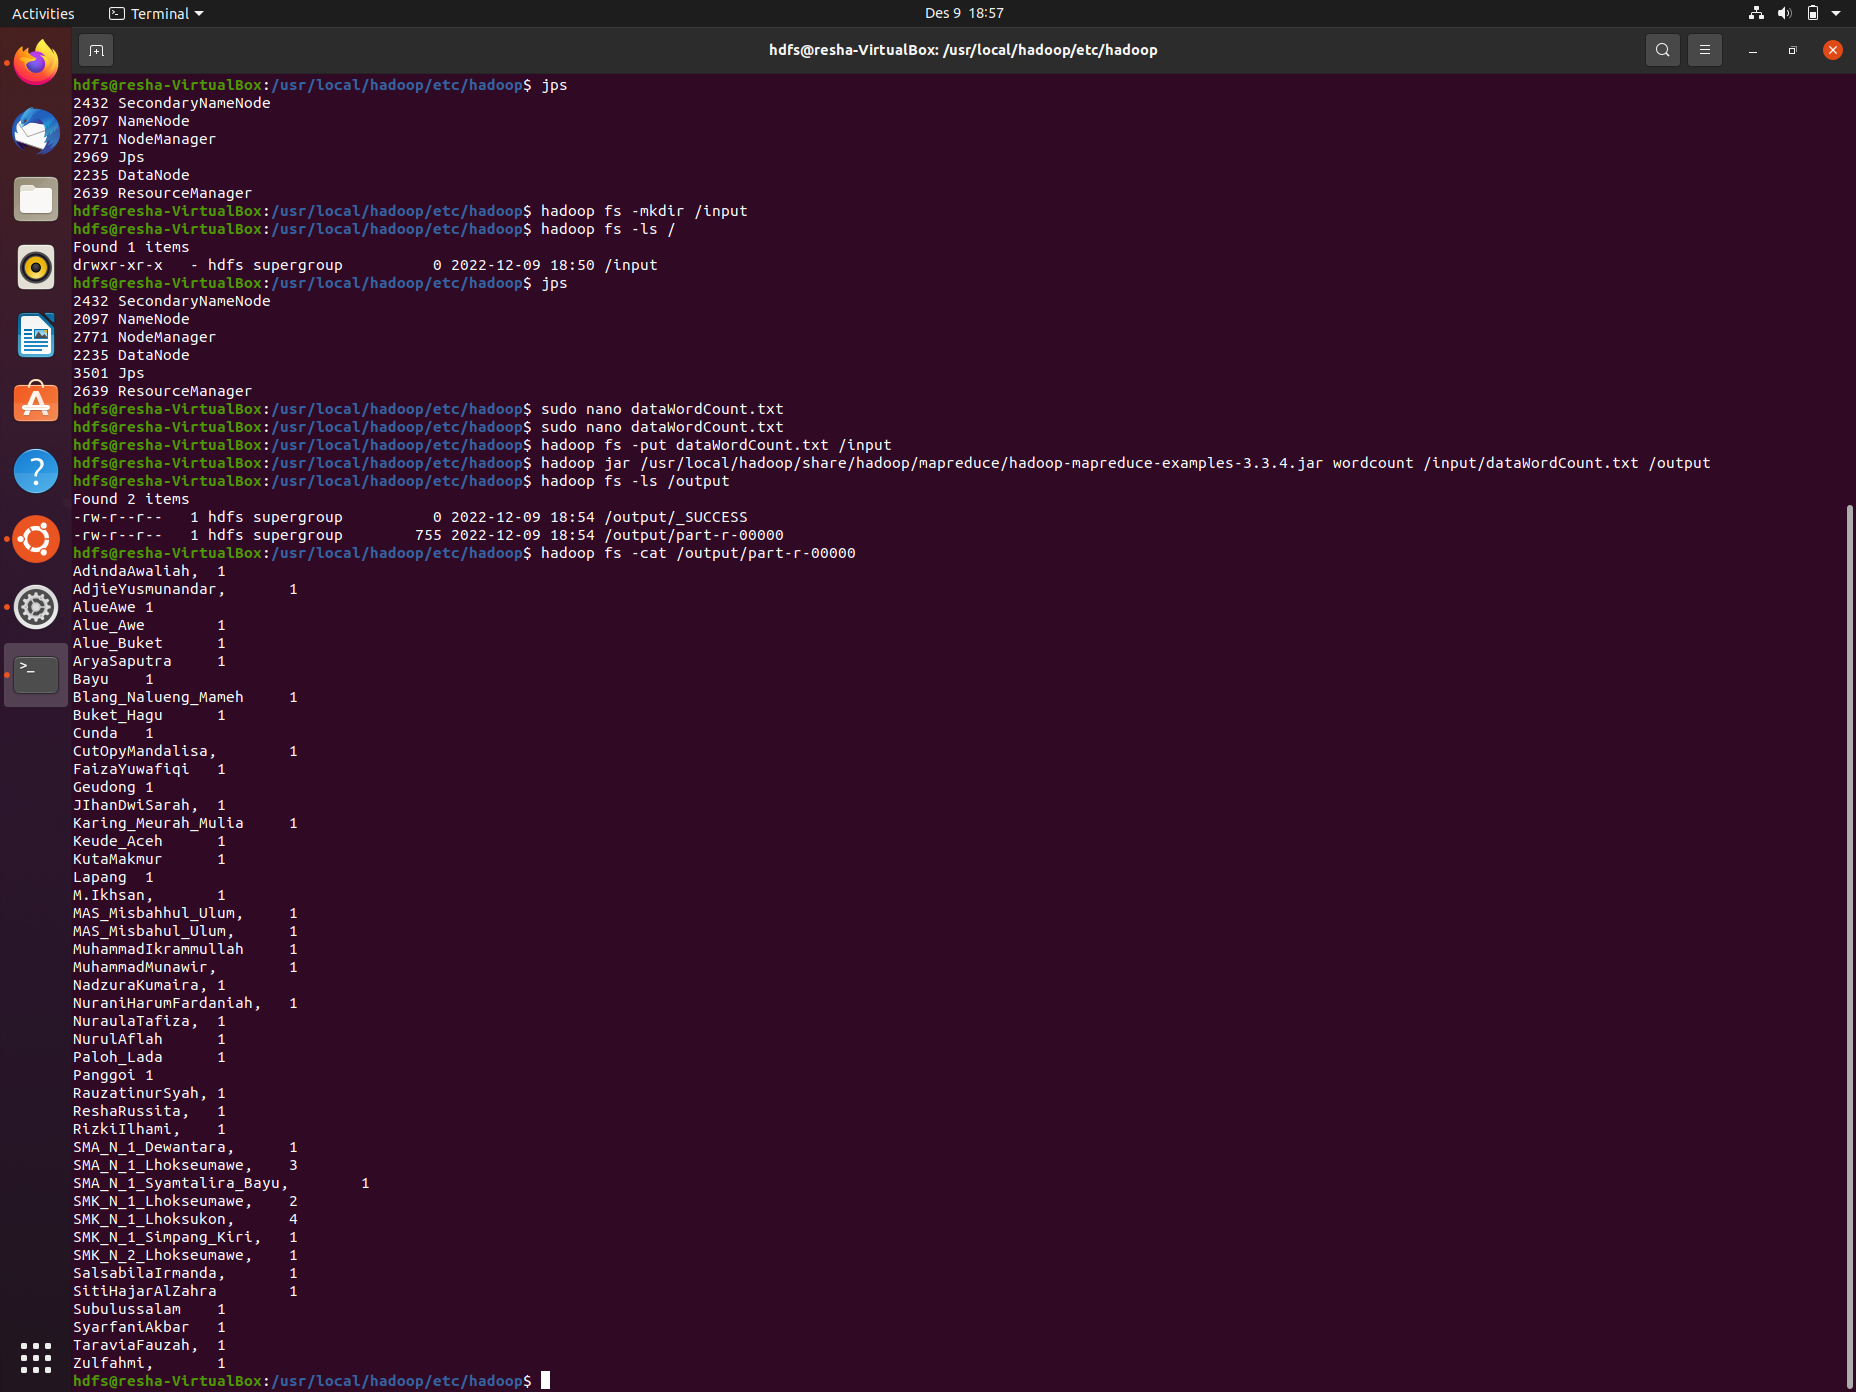
\includegraphics[width=\textwidth]{langkah6dan7-resha}
\caption{Hasil perhitungan dengan WordCount Hadoop berdasarkan data output}
\label{gam:perkuliahan-08-12}
\end{figure}

\item Kesimpulan
Pada Hadoop terdapat program untuk menghitung jumlah kata (WordCount) yang ada pada data. Untuk menghitung jumlah kata, saya sebagai praktikan melakukan input data terlebih dahulu, kemudian memprosesnya, sehingga menghasilkan data output. Data output tersebut yang digunakan untuk Hadoop menjalankan programnya yaitu WordCount.
Data yang saya input disini adalah data mahasiswa (nama, asal sekolah, dan alamat). Saat melihat hasil perhitungan pada data output, akan ditampilkan jumlah kata dari tiap-tiap nama, asal sekolah, dan alamat mahasiswa.

\end{enumerate}

\newday{\textbf{02 Desember 2022}}
\begin{enumerate}
\item Kendala dan Solusi
% jelaskan kendala dan penyebab yang dialami saat mengikuti praktikum serta solusi atau langkah-langkah yang telah dilakukan

\item Kesimpulan
% berikan kesimpulan dari praktikum yang telah dikerjkan

\end{enumerate}

\newday{\textbf{08 Desember 2022}}
\begin{enumerate}
\item Kendala dan Solusi
% jelaskan kendala dan penyebab yang dialami saat mengikuti praktikum serta solusi atau langkah-langkah yang telah dilakukan

\item Kesimpulan
% berikan kesimpulan dari praktikum yang telah dikerjkan

\end{enumerate}

\newday{\textbf{09 Desember 2022}}
\begin{enumerate}
\item Kendala dan Solusi
% jelaskan kendala dan penyebab yang dialami saat mengikuti praktikum serta solusi atau langkah-langkah yang telah dilakukan

\item Kesimpulan
% berikan kesimpulan dari praktikum yang telah dikerjkan

\end{enumerate}
\newthought{\textbf{Rizki Ilhami - 2020903430042 - TRKJ 3B}}

\newday{\textbf{1 Desember 2022}}
\begin{enumerate}
\item Kendala dan Solusi
% jelaskan kendala dan penyebab yang dialami saat mengikuti praktikum serta solusi atau langkah-langkah yang telah dilakukan

\item Kesimpulan
% berikan kesimpulan dari praktikum yang telah dikerjkan

\end{enumerate}

\newday{\textbf{2 Desember 2022}}
\begin{enumerate}
\item Kendala dan Solusi
% jelaskan kendala dan penyebab yang dialami saat mengikuti praktikum serta solusi atau langkah-langkah yang telah dilakukan

\item Kesimpulan
% berikan kesimpulan dari praktikum yang telah dikerjkan

\end{enumerate}
	
\newthought{\textbf{Salsabila Irmanda - 2020903430048 - TRKJ 3B}}
\newday{\textbf{1 Desember 2022}}
\begin{enumerate}
\item Kendala dan Solusi
% jelaskan kendala dan penyebab yang dialami saat mengikuti praktikum serta solusi atau langkah-langkah yang telah dilakukan

\item Kesimpulan
% berikan kesimpulan dari praktikum yang telah dikerjkan

\end{enumerate}


\newthought{\textbf{Adinda Awaliah - 2020903430004 - TRKJ 3B}}

\newday{\textbf{22 September 2022}}
\begin{enumerate}
\item Kendala dan Solusi
% jelaskan kendala dan penyebab yang dialami saat mengikuti praktikum serta solusi atau langkah-langkah yang telah dilakukan

\item Kesimpulan
% berikan kesimpulan dari praktikum yang telah dikerjkan

\end{enumerate}


\newthought{\textbf{Adinda Awaliah - 2020903430004 - TRKJ 3B}}

\newday{\textbf{22 September 2022}}
\begin{enumerate}
\item Kendala dan Solusi
% jelaskan kendala dan penyebab yang dialami saat mengikuti praktikum serta solusi atau langkah-langkah yang telah dilakukan

\item Kesimpulan
% berikan kesimpulan dari praktikum yang telah dikerjkan

\end{enumerate}


\newthought{\textbf{Taravia Fauzah- 2020903430054 - TRKJ 3B}}

\newday{\textbf{13-20 Oktober 2022} - Instalasi dan Konfigurasi Hadoop}
\begin{enumerate}
\item Kendala dan Solusi
% jelaskan kendala dan penyebab yang dialami saat mengikuti praktikum serta solusi atau langkah-langkah yang telah dilakukan
\newline praktikum pertama yaitu instalasi apache hadoop. selama mengerjakan praktikum mengikuti modul tidak ada kendala

\begin{figure}[!ht]
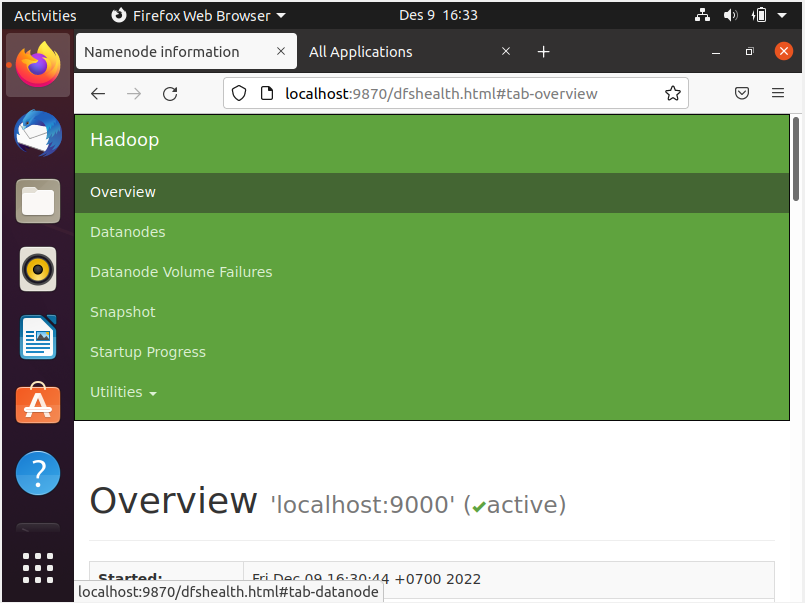
\includegraphics[width=\textwidth]{TaraviaFauzah/akses-localhost-9078}
\caption{hasil dari cek hadoop service}
\label{gam:perkuliahan15-9}
\end{figure}

\begin{figure}[!ht]
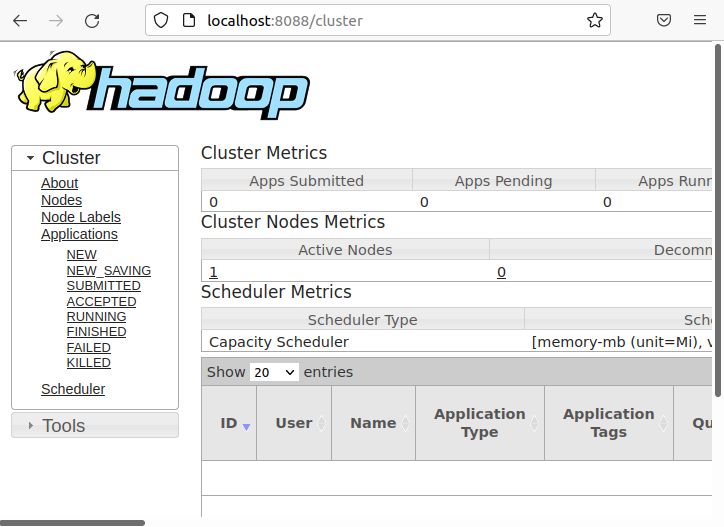
\includegraphics[width=\textwidth]{TaraviaFauzah/akses-localhost-8088}
\caption{hasil dari cek hadoop service}
\label{gam:perkuliahan15-9}
\end{figure}

\item Kesimpulan
% berikan kesimpulan dari praktikum yang telah dikerjkan
\newline Berhasil mendownload dan menginstal Apache hadoop dan sudah bisa di jalankan 
\end{enumerate}

\newday{\textbf{10 November 2022} - WordCount bawaan Hadoop}
\begin{enumerate}
\item Kendala dan Solusi
% jelaskan kendala dan penyebab yang dialami saat mengikuti praktikum serta solusi atau langkah-langkah yang telah dilakukan
\newline pada praktikum kali ini membuat program WordCount Bawaan Hadoop.pada saat praktikum tidak ada kendala hanya saja error karena salah menulis perintah.

\begin{figure}[!ht]
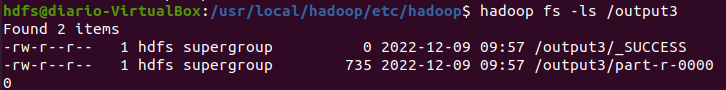
\includegraphics[width=\textwidth]{TaraviaFauzah/output}
\caption{hasil dari hadoop fs}
\label{gam:perkuliahan1-10}
\end{figure}

\begin{figure}[!ht]
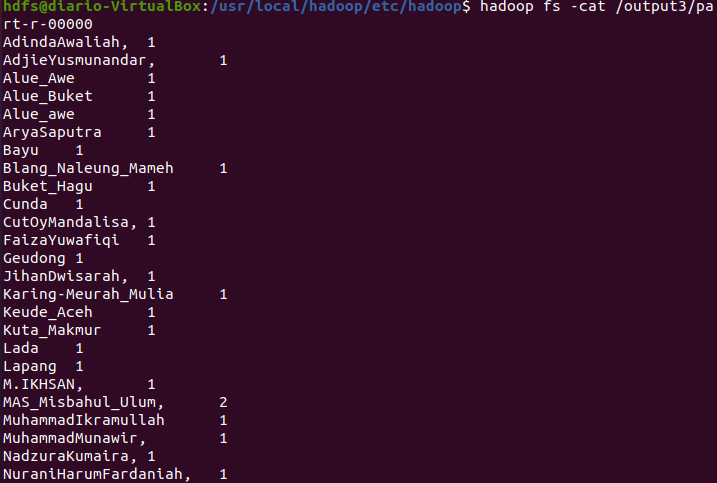
\includegraphics[width=\textwidth]{TaraviaFauzah/output1}
\caption{hasil dari hadoop fs}
\label{gam:perkuliahan1-10}
\end{figure}

\begin{figure}[!ht]
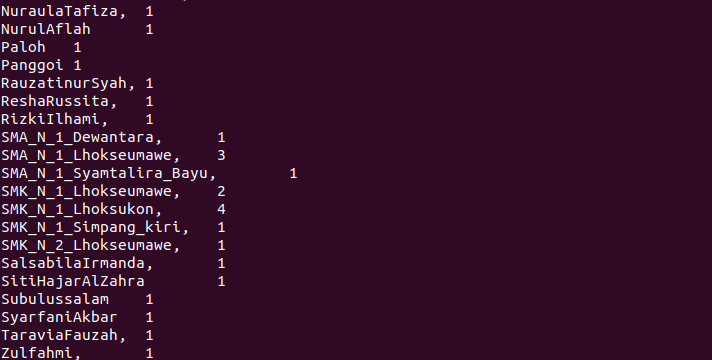
\includegraphics[width=\textwidth]{TaraviaFauzah/output1_1}
\caption{hasil dari hadoop fs}
\label{gam:perkuliahan1-10}
\end{figure}

\item Kesimpulan
% berikan kesimpulan dari praktikum yang telah dikerjkan
\newline langkah praktikum ini adalah untuk memahami proses cara kerja pada hadoop dalam memproses data input sehingga menghasikan sebuah output. wordcount adalah program untuk menghitung jumlah kata dalam inpu.

\end{enumerate}

\newday{\textbf{17 November 2022} - WordCount dengan Java}
\begin{enumerate}
\item Kendala dan Solusi
% jelaskan kendala dan penyebab yang dialami saat mengikuti praktikum serta solusi atau langkah-langkah yang telah dilakukan
\newline pada praktikum kali ini membuat program WordCount dengan java.pada saat praktikum memiliki error tapi errornya di sebabkan tidak teliti saat menulis codingan yang ada di modul.solusinya harus lebih teliti saat mengerjakan codingan tersebut.

\begin{figure}[!ht]
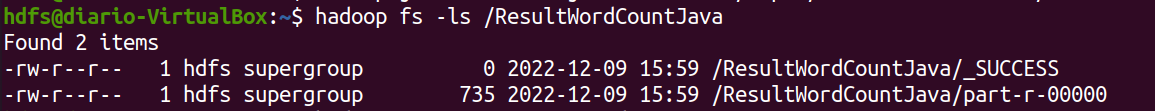
\includegraphics[width=\textwidth]{TaraviaFauzah/hasil1}
\caption{hasil dari hadoop fs WordCount}
\label{gam:perkuliahan2-12}
\end{figure}

\begin{figure}[!ht]
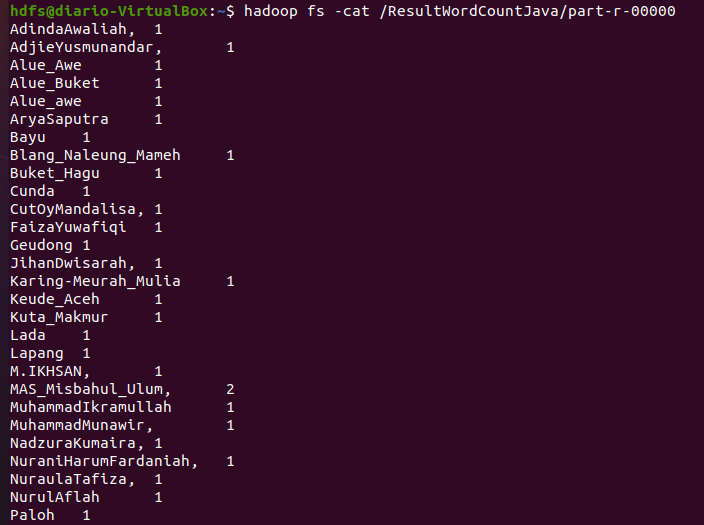
\includegraphics[width=\textwidth]{TaraviaFauzah/hasil2}
\caption{hasil dari hadoop fs WordCount}
\label{gam:perkuliahan2-12}
\end{figure}

\begin{figure}[!ht]
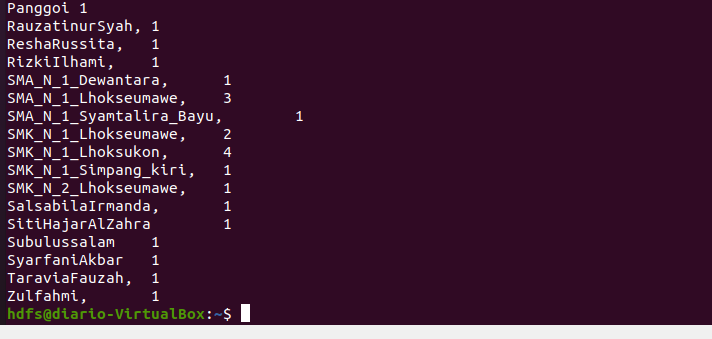
\includegraphics[width=\textwidth]{TaraviaFauzah/hasil2_2}
\caption{hasil dari hadoop fs WordCount}
\label{gam:perkuliahan2-12}
\end{figure}

\item Kesimpulan
% berikan kesimpulan dari praktikum yang telah dikerjkan
\newline berhasil menjalan program WordCount dengan java

\end{enumerate}

\newday{\textbf{24 November 2022} - instalasi apache Spark (Pyspark)}
\begin{enumerate}
\item Kendala dan Solusi
% jelaskan kendala dan penyebab yang dialami saat mengikuti praktikum serta solusi atau langkah-langkah yang telah dilakukan
\newline pada praktikum kali ini instalasi apache spark (pyspark)tidak ada kendala.

\begin{figure}[!ht]
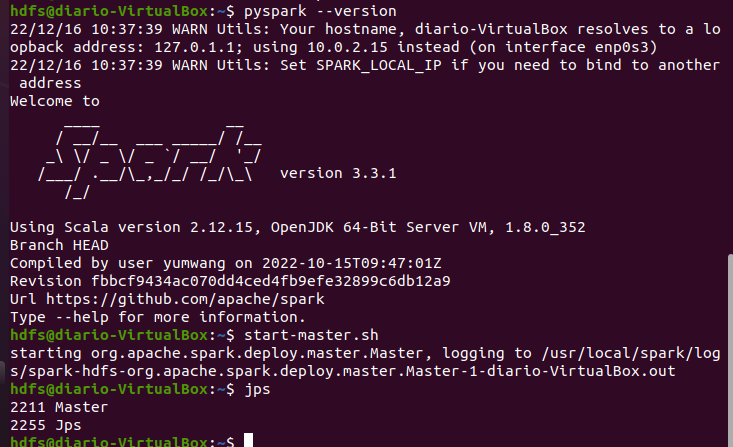
\includegraphics[width=\textwidth]{TaraviaFauzah/pyspark version}
\caption{hasil dari pyspark version}
\label{gam:perkuliahan2-15}
\end{figure}

\item Kesimpulan
% berikan kesimpulan dari praktikum yang telah dikerjkan
\newline berhasil menjalan pyspark yang sudah terinstall.
\end{enumerate}

\newday{\textbf{1 Desember 2022} - Program WordCount dengan Python}
\begin{enumerate}
\item Kendala dan Solusi
\newline pada praktikum kali ini membuat program wordcount dengan python,pada saat mengeisi codingan di nanonya harus lebih teliti supaya tidak terjadi error.

\begin{figure}[!ht]
\includegraphics[width=\textwidth]{TaraviaFauzah/hasil WordCountPython2}
\caption{lihat hasil dari WordCountPython }
\label{gam:perkuliahan2-15}
\end{figure}

\begin{figure}[!ht]
\includegraphics[width=\textwidth]{TaraviaFauzah/hasil WordCounPython1}
\caption{Cek hasil dari WordCountPython }
\label{gam:perkuliahan2-15}
\end{figure}

\item Kesimpulan
\newline berhasil membuat pemograman WordCount dengan Python.
\end{enumerate}

\newday{\textbf{8 Desember 2022} - Program WordCount dengan PySpark}
\begin{enumerate}
\item Kendala dan Solusi
\newline pada praktikum kali ini membuat program wordcount dengan pySpark,pada saat mengeisi codingan di nanonya harus lebih teliti supaya tidak terjadi error.

\begin{figure}[!ht]
\includegraphics[width=\textwidth]{TaraviaFauzah/hasil WordCountPySpark1}
\caption{cek hasil dari WordCountPySpark }
\label{gam:perkuliahan2-15}
\end{figure}

\begin{figure}[!ht]
\includegraphics[width=\textwidth]{TaraviaFauzah/hasil WordCountPySpark2}
\caption{lihat hasil dari WordCountPySpark }
\label{gam:perkuliahan2-15}
\end{figure}

\item Kesimpulan
\newline berhasil membuat pemograman WordCount dengan PySpark.
\end{enumerate}


\newthought{\textbf{Zulfahmi - 2020903430056 - TRKJ 3B}}

\newday{\textbf{01 Desember 2022}}
\begin{enumerate}
\item Kendala dan Solusi
% jelaskan kendala dan penyebab yang dialami saat mengikuti praktikum serta solusi atau langkah-langkah yang telah dilakukan

\item Kesimpulan
% berikan kesimpulan dari praktikum yang telah dikerjkan

\end{enumerate}

\newday{\textbf{02 Desember 2022}}
\begin{enumerate}
\item Kendala dan Solusi
% jelaskan kendala dan penyebab yang dialami saat mengikuti praktikum serta solusi atau langkah-langkah yang telah dilakukan

\item Kesimpulan
% berikan kesimpulan dari praktikum yang telah dikerjkan

\end{enumerate}

\newday{\textbf{08 Desember 2022}}
\begin{enumerate}
\item Kendala dan Solusi
% jelaskan kendala dan penyebab yang dialami saat mengikuti praktikum serta solusi atau langkah-langkah yang telah dilakukan

\item Kesimpulan
% berikan kesimpulan dari praktikum yang telah dikerjkan

\end{enumerate}

\clearpage
\bibliographystyle{plain}
\bibliography{lab_notes}

\end{document}

%%%%%%%%%%%%%%%%%%%%%%%%%%%%%%%%%%%%%%%%%%%%%%%%%%%%%%%%